% !TeX spellcheck = hu_HU
% !TeX encoding = UTF-8
% !TeX program = xelatex
% TODO Change language to en_GB (recommended) or en_US for English documents
\documentclass[12pt,a4paper,oneside]{report}             % Single-side
%\documentclass[11pt,a4paper,twoside,openright]{report}  % Duplex

% thanks to http://tex.stackexchange.com/a/47579/71109
\usepackage[light]{kpfonts}
\usepackage{ifxetex}
\usepackage{ifluatex}
\newif\ifxetexorluatex % a new conditional starts as false
\ifnum 0\ifxetex 1\fi\ifluatex 1\fi>0
   \xetexorluatextrue
\fi

\ifxetexorluatex
  \usepackage{fontspec}
\else
  \usepackage[T1]{fontenc}
  \usepackage[utf8]{inputenc}
  \usepackage[lighttt]{lmodern}
\fi

\usepackage[english,magyar]{babel} % Alapértelmezés szerint utoljára definiált nyelv lesz aktív, de később külön beállítjuk az aktív nyelvet.

%\usepackage{cmap}
\usepackage{amsfonts,amsmath} % Mathematical symbols. amssymb needed if no kpfonts


%\usepackage[ruled,boxed,resetcount,linesnumbered]{algorithm2e} % For pseudocodes. % beware: this is not compatible with LuaLaTeX, see http://tex.stackexchange.com/questions/34814/lualatex-and-algorithm2e
\usepackage{booktabs} % For publication quality tables for LaTeX
\usepackage{graphicx}

%\usepackage{fancyhdr}
%\usepackage{lastpage}

\usepackage{anysize}
%\usepackage{sectsty}
\usepackage{setspace} % For setting line spacing

\usepackage[unicode]{hyperref} % For hyperlinks in the generated document.
\usepackage{xcolor}
\usepackage{tcolorbox} 
\usepackage{listings} % For source code snippets.
\usepackage{lettrine}
\usepackage{pdfpages}

\usepackage[amsmath,thmmarks]{ntheorem} % Theorem-like environments.

\usepackage[hang]{caption}

\singlespacing

\newcommand{\selecthungarian}{
	\selectlanguage{magyar}
	\setlength{\parindent}{0em} % Nem akarom a behúzást
	\setlength{\parskip}{0em}
	\frenchspacing
}

\newcommand{\selectenglish}{
	\selectlanguage{english}
	\setlength{\parindent}{0em}
	\setlength{\parskip}{0.5em}
	\nonfrenchspacing
	\renewcommand{\figureautorefname}{Figure}
	\renewcommand{\tableautorefname}{Table}
	\renewcommand{\partautorefname}{Part}
	\renewcommand{\chapterautorefname}{Chapter}
	\renewcommand{\sectionautorefname}{Section}
	\renewcommand{\subsectionautorefname}{Section}
	\renewcommand{\subsubsectionautorefname}{Section}
}

\bibliographystyle{unsrtnat}
\usepackage[numbers]{natbib}
\usepackage{notoccite}

\usepackage{xspace}


%TODO Set the main variables
\newcommand{\vikszerzoVezeteknev}{Herőczi}
\newcommand{\vikszerzoKeresztnev}{Sándor}

\newcommand{\vikkonzulensAMegszolitas}{Dr.~}
\newcommand{\vikkonzulensAVezeteknev}{Stumpf Péter Pál}
\newcommand{\vikkonzulensAKeresztnev}{}

\newcommand{\vikkonzulensBMegszolitas}{}
\newcommand{\vikkonzulensBVezeteknev}{}
\newcommand{\vikkonzulensBKeresztnev}{}

\newcommand{\vikkonzulensCMegszolitas}{}
\newcommand{\vikkonzulensCVezeteknev}{}
\newcommand{\vikkonzulensCKeresztnev}{}

\newcommand{\vikcim}{Mikrovezérlő alapú autonóm fegyverrendszer tervezése és fejlesztése} % Cím
\newcommand{\viktanszek}{\bmeaut} % Tanszék
\newcommand{\vikdoktipus}{\msc} % Dokumentum típusa (\bsc vagy \msc)
\newcommand{\vikmunkatipusat}{diplomatervet} % a "hallgató nyilatkozat" részhez: szakdolgozatot vagy diplomatervet

%--------------------------------------------------------------------------------------
% TDK-specifikus változók
%--------------------------------------------------------------------------------------
\newcommand{\tdkszerzoB}{Második Szerző} % Második szerző neve; hagyd üresen, ha egyedül írtad a TDK-t.
\newcommand{\tdkev}{2024} % A dolgozat írásának éve (pl. "2014") (Ez OTDK-nál eltérhet az aktuális évtől.)

% További adatok az OTDK címlaphoz (BME-s TDK-hoz nem kell kitölteni)
\newcommand{\tdkevfolyamA}{IV} % Első szerző évfolyama, római számmal (pl. IV).
\newcommand{\tdkevfolyamB}{III} % Második szerző évfolyama, római számmal (pl. III).
\newcommand{\tdkkonzulensbeosztasA}{egyetemi tanár} % Első konzulens beosztása (pl. egyetemi docens)
\newcommand{\tdkkonzulensbeosztasB}{doktorandusz} % Második konzulens beosztása (pl. egyetemi docens)

\newcommand{\szerzoMeta}{\vikszerzoVezeteknev{} \vikszerzoKeresztnev} % egy szerző esetén
%\newcommand{\szerzoMeta}{\vikszerzoVezeteknev{} \vikszerzoKeresztnev, \tdkszerzoB} % két szerző esetén

%TODO Language configuration -- choose one
% Beállítások magyar nyelvű dolgozathoz
%--------------------------------------------------------------------------------------
% Elnevezések
%--------------------------------------------------------------------------------------
\newcommand{\bme}{Budapesti Műszaki és Gazdaságtudományi Egyetem}
\newcommand{\vik}{Villamosmérnöki és Informatikai Kar}

\newcommand{\bmemit}{Méréstechnika és Információs Rendszerek Tanszék}
\newcommand{\bmeaut}{Automatizálási és Alkalmazott Informatikai Tanszék}

\newcommand{\keszitette}{Készítette}
\newcommand{\konzulens}{Konzulens}

\newcommand{\bsc}{Szakdolgozat}
\newcommand{\msc}{Diplomaterv}
\newcommand{\tdk}{TDK dolgozat}
\newcommand{\bsconlab}{BSc Önálló laboratórium}
\newcommand{\msconlabi}{MSc Önálló laboratórium 1.}
\newcommand{\msconlabii}{MSc Önálló laboratórium 2.}

\newcommand{\pelda}{Példa}
\newcommand{\definicio}{Definíció}
\newcommand{\tetel}{Tétel}

\newcommand{\bevezetes}{Bevezetés}
\newcommand{\koszonetnyilvanitas}{Köszönetnyilvánítás}
\newcommand{\fuggelek}{Függelék}

% Opcionálisan átnevezhető címek
%\addto\captionsmagyar{%
%\renewcommand{\listfigurename}{Saját ábrajegyzék cím}
%\renewcommand{\listtablename}{Saját táblázatjegyzék cím}
%\renewcommand{\bibname}{Saját irodalomjegyzék név}
%}

\newcommand{\szerzo}{\vikszerzoVezeteknev{} \vikszerzoKeresztnev}
\newcommand{\vikkonzulensA}{\vikkonzulensAMegszolitas\vikkonzulensAVezeteknev{} \vikkonzulensAKeresztnev}
\newcommand{\vikkonzulensB}{\vikkonzulensBMegszolitas\vikkonzulensBVezeteknev{} \vikkonzulensBKeresztnev}
\newcommand{\vikkonzulensC}{\vikkonzulensCMegszolitas\vikkonzulensCVezeteknev{} \vikkonzulensCKeresztnev}

\newcommand{\selectthesislanguage}{\selecthungarian}

\bibliographystyle{huplain}

\def\lstlistingname{lista}

\newcommand{\appendixnumber}{6}  % a fofejezet-szamlalo az angol ABC 6. betuje (F) lesz

% Settings for English documents
%%--------------------------------------------------------------------------------------
% Elnevezések
%--------------------------------------------------------------------------------------
\newcommand{\bme}{Budapest University of Technology and Economics}
\newcommand{\vik}{Faculty of Electrical Engineering and Informatics}

\newcommand{\bmemit}{Department of Measurement and Information Systems}

\newcommand{\keszitette}{Author}
\newcommand{\konzulens}{Advisor}

\newcommand{\bsc}{Bachelor's Thesis}
\newcommand{\msc}{Master's Thesis}
\newcommand{\tdk}{Scientific Students' Association Report}
\newcommand{\bsconlab}{BSc Project Laboratory}
\newcommand{\msconlabi}{MSc Project Laboratory 1}
\newcommand{\msconlabii}{MSc Project Laboratory 2}

\newcommand{\pelda}{Example}
\newcommand{\definicio}{Definition}
\newcommand{\tetel}{Theorem}

\newcommand{\bevezetes}{Introduction}
\newcommand{\koszonetnyilvanitas}{Acknowledgements}
\newcommand{\fuggelek}{Appendix}

% Optional custom titles
%\addto\captionsenglish{%
%\renewcommand*{\listfigurename}{Your list of figures title}
%\renewcommand*{\listtablename}{Your list of tables title}
%\renewcommand*{\bibname}{Your bibliography title}
%}

\newcommand{\szerzo}{\vikszerzoKeresztnev{} \vikszerzoVezeteknev}
\newcommand{\vikkonzulensA}{\vikkonzulensAMegszolitas\vikkonzulensAKeresztnev{} \vikkonzulensAVezeteknev}
\newcommand{\vikkonzulensB}{\vikkonzulensBMegszolitas\vikkonzulensBKeresztnev{} \vikkonzulensBVezeteknev}
\newcommand{\vikkonzulensC}{\vikkonzulensCMegszolitas\vikkonzulensCKeresztnev{} \vikkonzulensCVezeteknev}

\newcommand{\selectthesislanguage}{\selectenglish}

\bibliographystyle{plainnat}

\newcommand{\ie}{i.e.\@\xspace}
\newcommand{\Ie}{I.e.\@\xspace}
\newcommand{\eg}{e.g.\@\xspace}
\newcommand{\Eg}{E.g.\@\xspace}
\newcommand{\etal}{et al.\@\xspace}
\newcommand{\etc}{etc.\@\xspace}
\newcommand{\vs}{vs.\@\xspace}
\newcommand{\viz}{viz.\@\xspace} % videlicet
\newcommand{\cf}{cf.\@\xspace} % confer
\newcommand{\Cf}{Cf.\@\xspace}
\newcommand{\wrt}{w.r.t.\@\xspace} % with respect to
\newcommand{\approximately}{approx.\@\xspace}

\newcommand{\appendixnumber}{1}  % a fofejezet-szamlalo az angol ABC 1. betuje (A) lesz


%--------------------------------------------------------------------------------------
% Page layout setup
%--------------------------------------------------------------------------------------
% we need to redefine the pagestyle plain
% another possibility is to use the body of this command without \fancypagestyle
% and use \pagestyle{fancy} but in that case the special pages
% (like the ToC, the References, and the Chapter pages)remain in plane style

\pagestyle{plain}
\marginsize{35mm}{25mm}{15mm}{15mm}

\setcounter{tocdepth}{3}
%\sectionfont{\large\upshape\bfseries}
\setcounter{secnumdepth}{3}

\sloppy % Margón túllógó sorok tiltása.
\widowpenalty=10000 \clubpenalty=10000 %A fattyú- és árvasorok elkerülése
\def\hyph{-\penalty0\hskip0pt\relax} % Kötőjeles szavak elválasztásának engedélyezése
\graphicspath{{./figures/}}


%--------------------------------------------------------------------------------------
% Setup hyperref package
%--------------------------------------------------------------------------------------
\hypersetup{
    % bookmarks=true,            % show bookmarks bar?
    unicode=true,              % non-Latin characters in Acrobat's bookmarks
    pdftitle={\vikcim},        % title
    pdfauthor={\szerzoMeta},    % author
    pdfsubject={\vikdoktipus}, % subject of the document
    pdfcreator={\szerzoMeta},   % creator of the document
    pdfproducer={},    % producer of the document
    pdfkeywords={},    % list of keywords (separate then by comma)
    pdfnewwindow=true,         % links in new window
    colorlinks=true,           % false: boxed links; true: colored links
    linkcolor=black,           % color of internal links
    citecolor=black,           % color of links to bibliography
    filecolor=black,           % color of file links
    urlcolor=black             % color of external links
}


%--------------------------------------------------------------------------------------
% Set up listings
%--------------------------------------------------------------------------------------
\definecolor{lightgray}{rgb}{0.95,0.95,0.95}
\lstset{
	basicstyle=\scriptsize\ttfamily, % print whole listing small
	keywordstyle=\color{black}\bfseries, % bold black keywords
	identifierstyle=, % nothing happens
	% default behavior: comments in italic, to change use
	% commentstyle=\color{green}, % for e.g. green comments
	stringstyle=\scriptsize,
	showstringspaces=false, % no special string spaces
	aboveskip=3pt,
	belowskip=3pt,
	backgroundcolor=\color{lightgray},
	columns=flexible,
	keepspaces=true,
	escapeinside={(*@}{@*)},
	captionpos=b,
	breaklines=true,
	frame=single,
	float=!ht,
	tabsize=2,
	literate=*
		{á}{{\'a}}1	{é}{{\'e}}1	{í}{{\'i}}1	{ó}{{\'o}}1	{ö}{{\"o}}1	{ő}{{\H{o}}}1	{ú}{{\'u}}1	{ü}{{\"u}}1	{ű}{{\H{u}}}1
		{Á}{{\'A}}1	{É}{{\'E}}1	{Í}{{\'I}}1	{Ó}{{\'O}}1	{Ö}{{\"O}}1	{Ő}{{\H{O}}}1	{Ú}{{\'U}}1	{Ü}{{\"U}}1	{Ű}{{\H{U}}}1
}


%--------------------------------------------------------------------------------------
% Set up theorem-like environments
%--------------------------------------------------------------------------------------
% Using ntheorem package -- see http://www.math.washington.edu/tex-archive/macros/latex/contrib/ntheorem/ntheorem.pdf

\theoremstyle{plain}
\theoremseparator{.}
\newtheorem{example}{\pelda}

\theoremseparator{.}
%\theoremprework{\bigskip\hrule\medskip}
%\theorempostwork{\hrule\bigskip}
\theorembodyfont{\upshape}
\theoremsymbol{{\large \ensuremath{\centerdot}}}
\newtheorem{definition}{\definicio}

\theoremseparator{.}
%\theoremprework{\bigskip\hrule\medskip}
%\theorempostwork{\hrule\bigskip}
\newtheorem{theorem}{\tetel}


%--------------------------------------------------------------------------------------
% Some new commands and declarations
%--------------------------------------------------------------------------------------
\newcommand{\code}[1]{{\tcbox{\upshape\ttfamily\footnotesize\indent #1}}}

\newcommand{\doi}[1]{DOI: \href{http://dx.doi.org/\detokenize{#1}}{\raggedright{\texttt{\detokenize{#1}}}}} % A hivatkozások közt így könnyebb DOI-t megadni.

\newcommand{\w}[1]{\; \mathrm{#1}}
\newcommand{\q}[1]{\; \left[\mathrm{#1}\right]}

\DeclareMathOperator*{\argmax}{arg\,max}
%\DeclareMathOperator*[1]{\floor}{arg\,max}
\DeclareMathOperator{\sign}{sgn}
\DeclareMathOperator{\rot}{rot}

\tcbset{on line, 
	boxsep=1pt, left=0pt,right=0pt,top=0pt,bottom=0pt,
	colframe=white,colback=lightgray
}

%--------------------------------------------------------------------------------------
% Setup captions
%--------------------------------------------------------------------------------------
\captionsetup[figure]{
	width=.75\textwidth,
	aboveskip=10pt}

\renewcommand{\captionlabelfont}{\bf}
%\renewcommand{\captionfont}{\footnotesize\it}

%--------------------------------------------------------------------------------------
% Hyphenation exceptions
%--------------------------------------------------------------------------------------
\hyphenation{Shakes-peare Mar-seilles ár-víz-tű-rő tü-kör-fú-ró-gép}


\author{\vikszerzo}
\title{\viktitle}

%--------------------------------------------------------------------------------------
% Table of contents and the main text
%--------------------------------------------------------------------------------------
\begin{document}

\pagenumbering{gobble}

%TODO These includes define guidelines -- remove these
%~~~~~~~~~~~~~~~~~~~~~~~~~~~~~~~~~~~~~~~~~~~~~~~~~~~~~~~~~~~~~~~~~~~~~~~~~~~~~~~~~~~~~~

%--------------------------------------------------------------------------------------
% Feladatkiiras (a tanszeken atveheto, kinyomtatott valtozat)
%--------------------------------------------------------------------------------------
\clearpage

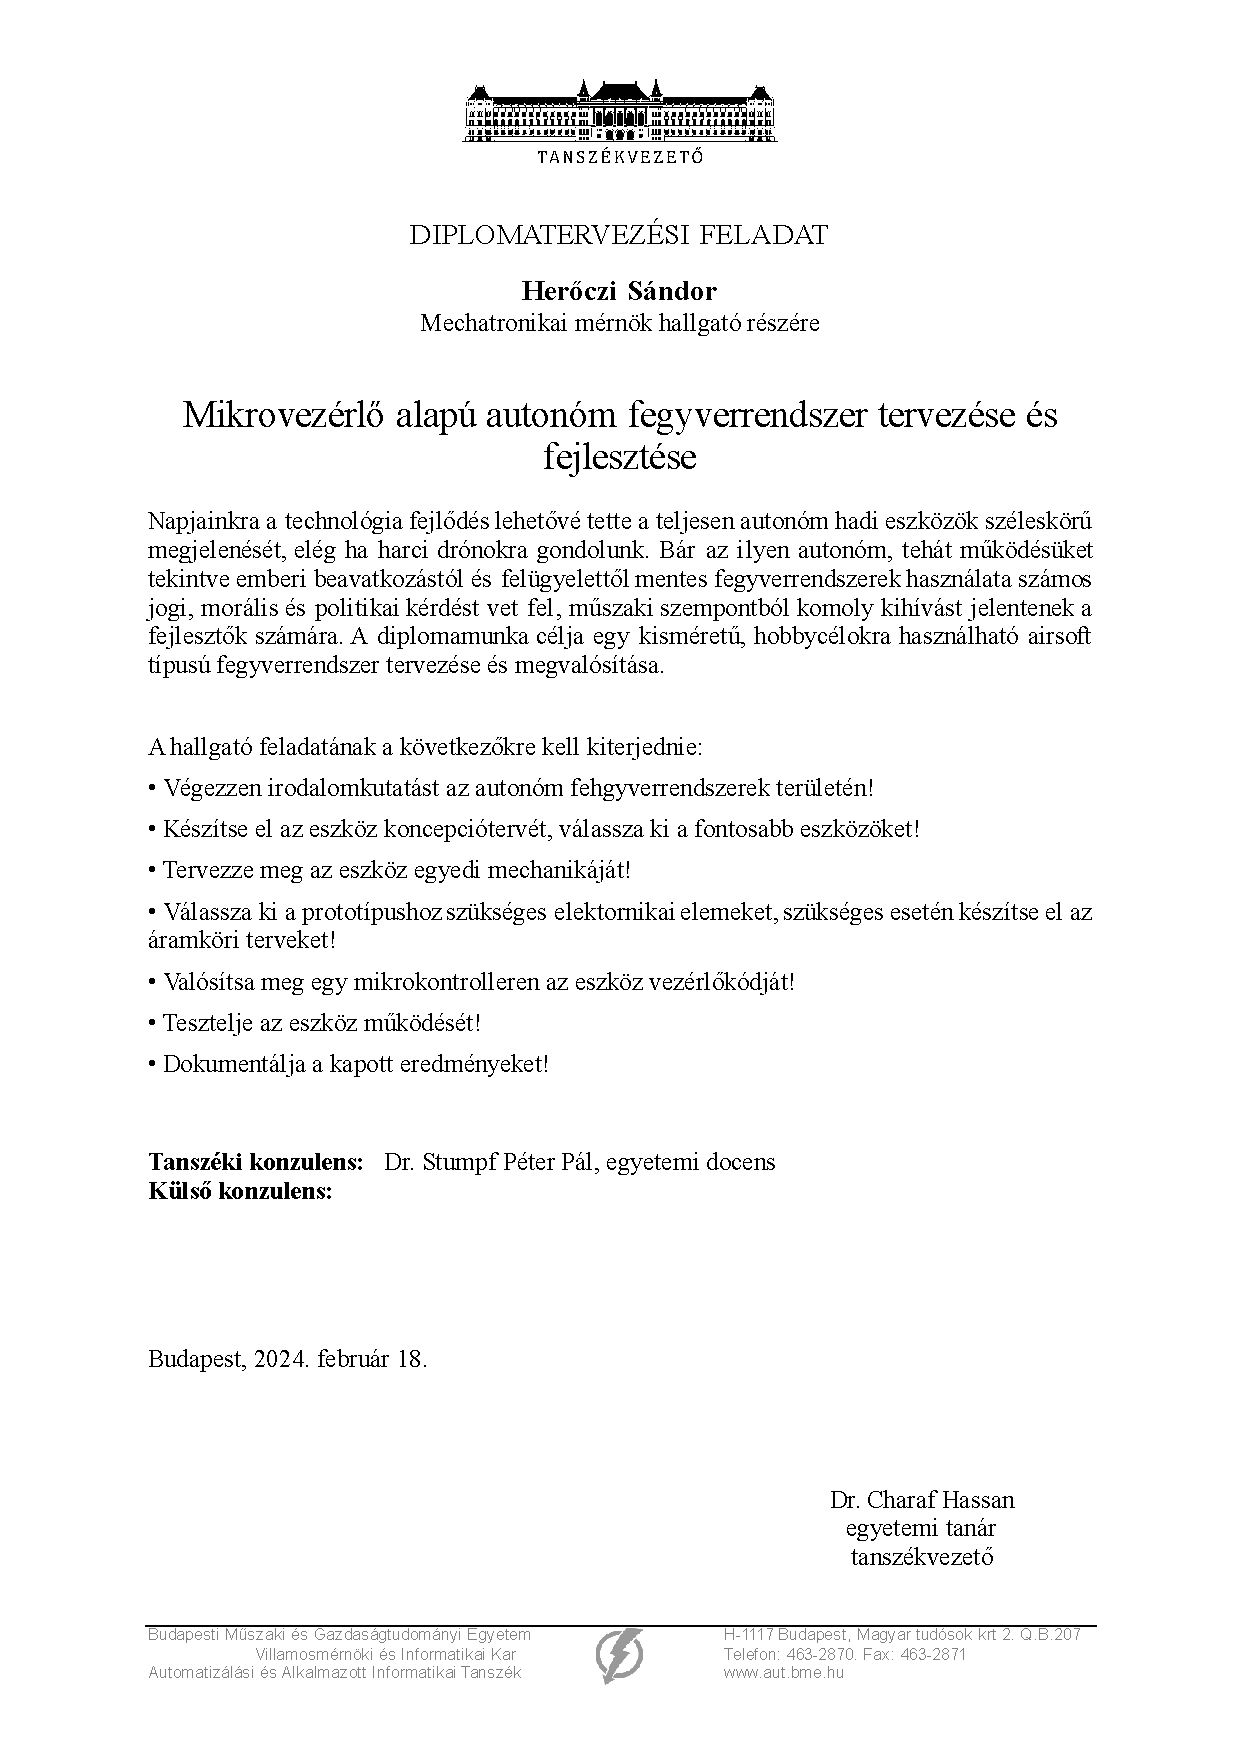
\includepdf[pages=-]{feladatkiiras.pdf}

\selectthesislanguage

%TODO Titlepage -- choose one from below
%~~~~~~~~~~~~~~~~~~~~~~~~~~~~~~~~~~~~~~~~~~~~~~~~~~~~~~~~~~~~~~~~~~~~~~~~~~~~~~~~~~~~~~
\hypersetup{pageanchor=false}
%--------------------------------------------------------------------------------------
%	The title page
%--------------------------------------------------------------------------------------
\begin{titlepage}
\begin{center}

\includegraphics[width=60mm,keepaspectratio]{figures/bme_logo.pdf}\\
\vspace{0.3cm}
\textbf{\bme}\\
\textmd{\vik}\\
\textmd{\viktanszek}\\[5cm]

\vspace{0.4cm}
{\huge \bfseries \vikcim}\\[0.8cm]
\vspace{0.5cm}
\textsc{\Large \vikdoktipus}\\[4cm]

{
	\renewcommand{\arraystretch}{0.85}
	\begin{tabular}{cc}
	 \makebox[7cm]{\emph{\keszitette}} & \makebox[7cm]{\emph{\konzulens}} \\ \noalign{\smallskip}
	 \makebox[7cm]{\szerzo} & \makebox[7cm]{\vikkonzulensA} \\
	  & \makebox[7cm]{\vikkonzulensB} \\
	  & \makebox[7cm]{\vikkonzulensC} \\
	\end{tabular}
}

\vfill
{\large \today}
\end{center}
\end{titlepage}
\hypersetup{pageanchor=false}

		   % Szakdolgozat/Diplomaterv címlap
%%% TDK címlap
\begin{titlepage}
  \begin{center}  
  
\includegraphics[width=7cm]{./figures/bme_logo.pdf}
  \vspace{0.3cm}
  
  \bme \\
  \vik \\
  \viktanszek \\
  \vspace{5cm}
  
  \huge {\vikcim}
  \vspace{1.5cm}
  
  \large {\textbf{\tdk}}
  \vfill
    
  {\Large 
  	\keszitette: \\ \vspace{0.3cm}
  	\szerzo \\
	\tdkszerzoB \\
  	\vspace{1.5cm}
  	\konzulens: \\ \vspace{0.3cm}
  	\vikkonzulensA \\
  	\vikkonzulensB \\
  }
  
  \vspace{2cm}
  \large {\tdkev}
 \end{center}
\end{titlepage}
%% Címlap vége
	% TDK címlap
%%% OTDK külső címlap
\begin{titlepage}
  	$\;$ 
	\vspace{5cm}
	
	\begin{center}
	\Huge
	\textbf{TDK-dolgozat}\let\thefootnote\relax\footnote{A dolgozat bemutatását a XXXXXXXXX  ``Lorem ipsum dolor sit amet'' című program támogatta.}
	\end{center}
	
	\vspace{13cm}
	
	\Large
	\hspace{8cm} \szerzo
	
	\hspace{8cm} \tdkszerzoB
	
	\hspace{8cm} \tdkev.
\end{titlepage}

\newpage
\thispagestyle{empty}


%% OTDK belső címlap
\begin{titlepage}
  \begin{center}  
  
\includegraphics[width=7cm]{./figures/bme_logo.pdf}
  \vspace{0.3cm}
  
  \bme \\
  \vik \\
  \viktanszek \\
  \vspace{3.5cm}
  
  \huge {\vikcim}
  \vspace{1.5cm}
  
  \large {\textbf{\vikdoktipus}}
  \vfill
    
  {\Large 
  	{\large \keszitette:} \\ \vspace{0.2cm}
  	\szerzo \\ \tdkevfolyamA. évfolyam \\
	\vspace{0.5cm}
	\tdkszerzoB \\ \tdkevfolyamB. évfolyam \\
  	\vspace{1.5cm}
  	{\large \konzulens:} \\ \vspace{0.2cm}
  	\vikkonzulensA,\\ \tdkkonzulensbeosztasA \\
  	\vspace{0.5cm}
  	\vikkonzulensB,\\ \tdkkonzulensbeosztasB \\
  }
  
  \vspace{2cm}
  \large {\tdkev.}
  
 \end{center}
\end{titlepage}   % OTDK címlap


% Table of Contents
%~~~~~~~~~~~~~~~~~~~~~~~~~~~~~~~~~~~~~~~~~~~~~~~~~~~~~~~~~~~~~~~~~~~~~~~~~~~~~~~~~~~~~~
\tableofcontents\vfill


% Declaration and Abstract
%~~~~~~~~~~~~~~~~~~~~~~~~~~~~~~~~~~~~~~~~~~~~~~~~~~~~~~~~~~~~~~~~~~~~~~~~~~~~~~~~~~~~~~
\selectlanguage{magyar}
\pagenumbering{gobble}
%--------------------------------------------------------------------------------------
% Nyilatkozat
%--------------------------------------------------------------------------------------
\begin{center}
\large
\textbf{HALLGATÓI NYILATKOZAT}\\
\end{center}

Alulírott \emph{\vikszerzoVezeteknev{} \vikszerzoKeresztnev}, szigorló hallgató kijelentem, hogy ezt a \vikmunkatipusat{} meg nem engedett segítség nélkül, saját magam készítettem, csak a megadott forrásokat (szakirodalom, eszközök stb.) használtam fel. Minden olyan részt, melyet szó szerint, vagy azonos értelemben, de átfogalmazva más forrásból átvettem, egyértelműen, a forrás megadásával megjelöltem.

Hozzájárulok, hogy a jelen munkám alapadatait (szerző(k), cím, angol és magyar nyelvű tartalmi kivonat, készítés éve, konzulens(ek) neve) a BME VIK nyilvánosan hozzáférhető elektronikus formában, a munka teljes szövegét pedig az egyetem belső hálózatán keresztül (vagy autentikált felhasználók számára) közzétegye. Kijelentem, hogy a benyújtott munka és annak elektronikus verziója megegyezik. Dékáni engedéllyel titkosított diplomatervek esetén a dolgozat szövege csak 3 év eltelte után válik hozzáférhetővé.

\begin{flushleft}
\vspace*{1cm}
Budapest, \today
\end{flushleft}

\begin{flushright}
 \vspace*{1cm}
 \makebox[7cm]{\rule{6cm}{.4pt}}\\
 \makebox[7cm]{\emph{\vikszerzoVezeteknev{} \vikszerzoKeresztnev}}\\
 \makebox[7cm]{hallgató}
\end{flushright}
\thispagestyle{empty}

\vfill
\clearpage
\thispagestyle{empty} % an empty page

\selectthesislanguage
 %TODO Hallgatói nyilatkozat -- TDK és OTDK esetén törlendő!
\pagenumbering{roman}
\setcounter{page}{1}

\selecthungarian

%----------------------------------------------------------------------------
% Abstract in Hungarian
%----------------------------------------------------------------------------
\chapter*{Kivonat}\addcontentsline{toc}{chapter}{Kivonat}

A diplomamunkám célja egy autonóm fegyverrendszer fejlesztése és elkészítése, amely funkciójában hasonlít a valós, éles helyzetben alkalmazott rendszerekhez. Ez annyit takar, hogy a fegyvernek képesnek kell egy bizonyos méretű területet belátni, ebben felismerni és azonosítani a célpontokat, majd tüzelni, vagy engedélyt kérni tüzelésre. Ezentúl szükséges funkciója a manuális vezérlés, amely segítségével az operátor valós időben tudja távolról irányítani az eszközt, egy asztali számítógép segítségével.\\

Az eszköz alkatrészei 3D nyomtatási technológiával készültek, a kötőelemeket, csapágyakat és elektronikai elemeket kivéve, első feladatom ezek nyomtatáshelyes megtervezése volt. A következő lépés a hardver és elektronikai rendszer tervezése volt, majd a szükséges modulok, szenzorok, mikrovezérlő kiválasztása és megrendelése. Az utolsó alfeladat pedig a szoftver fejlesztése, amely jelentette mind a beágyazott vezérlő szoftvert, és a számítógépen futó felhasználói felületet is.\\

A projekt megvalósítása során végig sok időt emésztett fel a rendszer tesztelése, amelyet párhuzamosan kellett végezni a későbbi alfeladatok tervezésével. Kihívást jelentett a megfelelően részletes szakirodalom felkutatása is, ugyanis a valós megoldások paramétereit gyakran nem teszik elérhetővé civilek számára, illetve a jelenleg folyó fejlesztések is titkosítottak.\\

Úgy gondolom, a téma interdiszciplináris jellegét tekintve jól illik a mechatronikai tanulmányaiba, ugyanis egyaránt érinti a műszaki mechanika,  a gyártástechnológia, a szoftverkészítés és a jelfeldolgozás területeit.\\

Diplomamunkám eredményeként megvalósítok egy működő prototípust, amit előadás keretében fogok bemutatni. Végül pedig kitérek az esetleges hibákra amiket elkövettem, a tanulságokra és a továbbfejlesztési lehetőségekre.


\vfill
\selectenglish


%----------------------------------------------------------------------------
% Abstract in English
%----------------------------------------------------------------------------
\chapter*{Abstract}\addcontentsline{toc}{chapter}{Abstract}

The aim of my thesis is to develop and build an autonomous weapon system that functions similarly to real-world systems used in live scenarios. This means that the weapon must be able to monitor a designated area, recognize and identify targets, then fire or request permission to fire. Additionally, a necessary feature is manual control, allowing the operator to remotely control the device in real-time using a desktop computer.\\

The components of the device were created using 3D printing technology, except for the fasteners, bearings, and electronic elements. My first task was to design these components to be suitable for printing. The next step was to design the hardware and electronic system, followed by selecting and ordering the necessary modules, sensors, and microcontroller. The final subtask was the development of the software, which included both the embedded controller software and the user interface running on a computer.\\

Throughout the project, significant time was consumed by system testing, which had to be carried out simultaneously with the planning of subsequent subtasks. A challenge was also posed by finding sufficiently detailed technical literature, as the parameters of real-world solutions are often not made available to civilians, and current developments are often classified.\\

I believe that the interdisciplinary nature of this topic fits well with my mechatronics studies, as it encompasses areas such as mechanical engineering, manufacturing technology, software development, and signal processing.\\

As a result of my thesis, I will produce a working prototype, which I will present during my final defense. Lastly, I will address any mistakes I made, lessons learned, and possibilities for future development.

\vfill
\selectthesislanguage

\newcounter{romanPage}
\setcounter{romanPage}{\value{page}}
\stepcounter{romanPage}    %TODO Összefoglaló -- TDK és OTDK esetén nem kötelező


% The main part of the thesis
%~~~~~~~~~~~~~~~~~~~~~~~~~~~~~~~~~~~~~~~~~~~~~~~~~~~~~~~~~~~~~~~~~~~~~~~~~~~~~~~~~~~~~~
\pagenumbering{arabic}

%TODO import your own content
%----------------------------------------------------------------------------
\chapter{\bevezetes}
%----------------------------------------------------------------------------

\section{Motiváció és háttér}

\lettrine{E}zt a projektet nem a tanszéki diplomamunkatémák listáján találtam, hanem én kerestem hozzá konzulest. Szeretném ezért először megemlíteni a személyes motivációmat, és érdekeltségeimet vele kapcsolatban. Mint a legtöbb reál beállítottságú fiú, engem is fiatal korom óta érdekel a technológia, a járművek, a gépek, vagy a fegyverek. Ezek közös metszéspontja a haditechnológia, ami általában jóval fejlettebb, mint amivel a civil életben találkozhatunk. Ez az érdeklődés megmaradt kamaszkoromra is, amikor a videojátékok által új ingerként értek a \textsl{Team Fortress 2}-ben és a \textsl{Portal}-ban lévő ún. \textbf{Sentry Gun}-ok. \\[5mm]



\begin{figure}[h!]
	\centering
	\begin{minipage}{.5\textwidth}
		\centering
		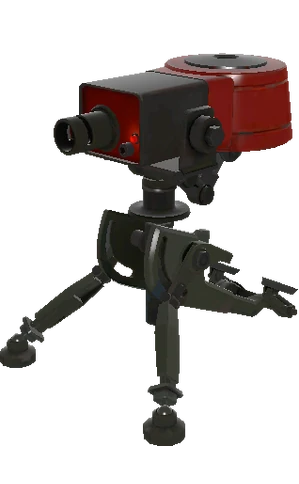
\includegraphics[width=0.8\linewidth]{irod_tf2} 
		\caption{TF2 Sentry Gun \cite{tf2}}
		\label{fig:irod_tf2}
	\end{minipage}%
	\begin{minipage}{.5\textwidth}
		\centering
		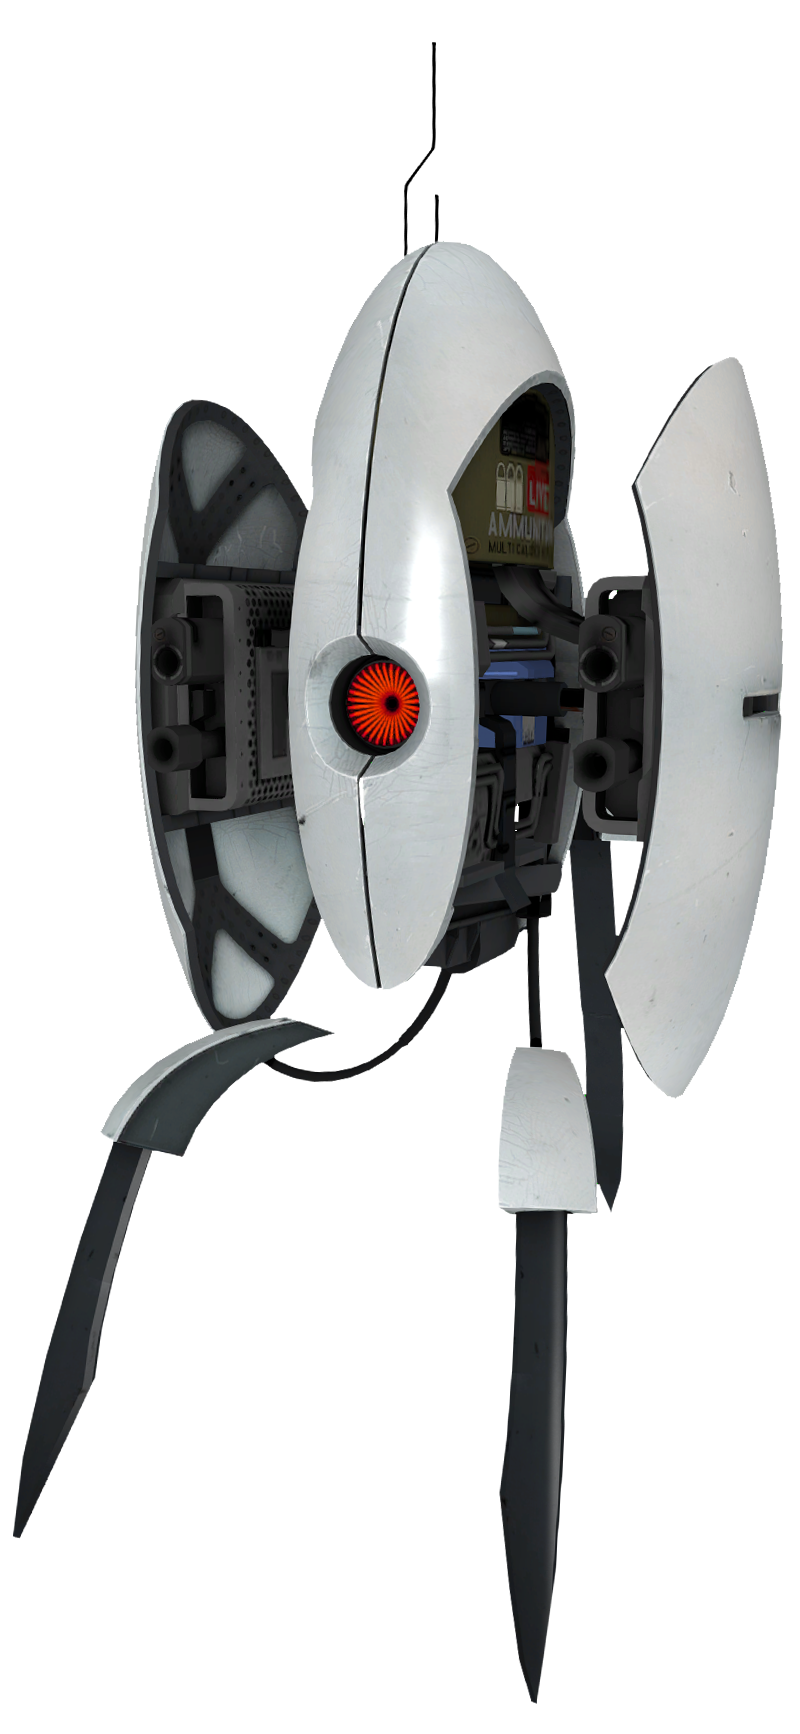
\includegraphics[width=0.6\linewidth]{irod_portal} 
		\caption{Portal Sentry Gun \cite{portal}}
		\label{fig:irod_portal}
	\end{minipage}
\end{figure}

Ezek olyan lövegek , amelyek a lábukon állva képesek voltak forogni, és ha az ellenség a látóterükbe jutott, akkor arra tüzet nyitottak. Nyilván játékokról van szó, tehát mindig azt hittem hogy ez csak a jövő technológiája, de nem sokkal később rá kellett jönnöm, hogy nagyon is valódiak. Ezután, mikor már egyetemre jártunk, egy barátommal egyre komolyabban kezdtünk beszélgetni arról, hogy esetleg mi is tudnánk egyet építeni. Végül az egyetemi éveim végére érve el is jött a tökéletes alkalom, hogy megvalósítsam régi álmomat. \\

A szentimentalitást félretéve, természetesen nem választottam volna ezt a témát, ha nem lenne a tanulmányaim szempontjából is releváns. Úgy gondolom, ez a projekt a mechatronika oktatás sok fontos elemét magában hordozza. A feladat a mechanikai konstrukcióval kezdődik és a CAD modellezéssel, amely a gépészeti oldalát hasznosítja a képzésünknek. Foglakozni kell a hardverrel, amihez elektronikai ismeretek szükségesek. Végül pedig a szoftvert kell lefejleszteni, ami informatikai szempontból érdekes. Ráadásul az egész beágyazott környezetben történik, ami miatt még relevánsabb az \textsl{intelligens beágyazott rendszerek} specializációmhoz. Véleményem szerint a projekt nehézsége és kihívása nem az egyes alfeladatokban rejlik, hanem az egész rendszer integrálásában, egymáshoz illesztésében. \\

Szintén fontosnak tartom megemlíteni, hogy a feladat lehetőséget ad megismerni és használni pár igen modern technológiát. A közelmúltban elérhetővé (és megfizethetővé) váltak civil felhasználásra a 3D nyomtatók, valamint a fejlődés a \textsl{Deep Learning} algoritmusok terén nagyban befolyásolta a gépi látás szakterületét is. Többek között a célom, hogy jobban megismerkedjek ezekkel a módszerekkel, és alkalmazzam őket.\\

\begin{figure}[h!]
	\centering
	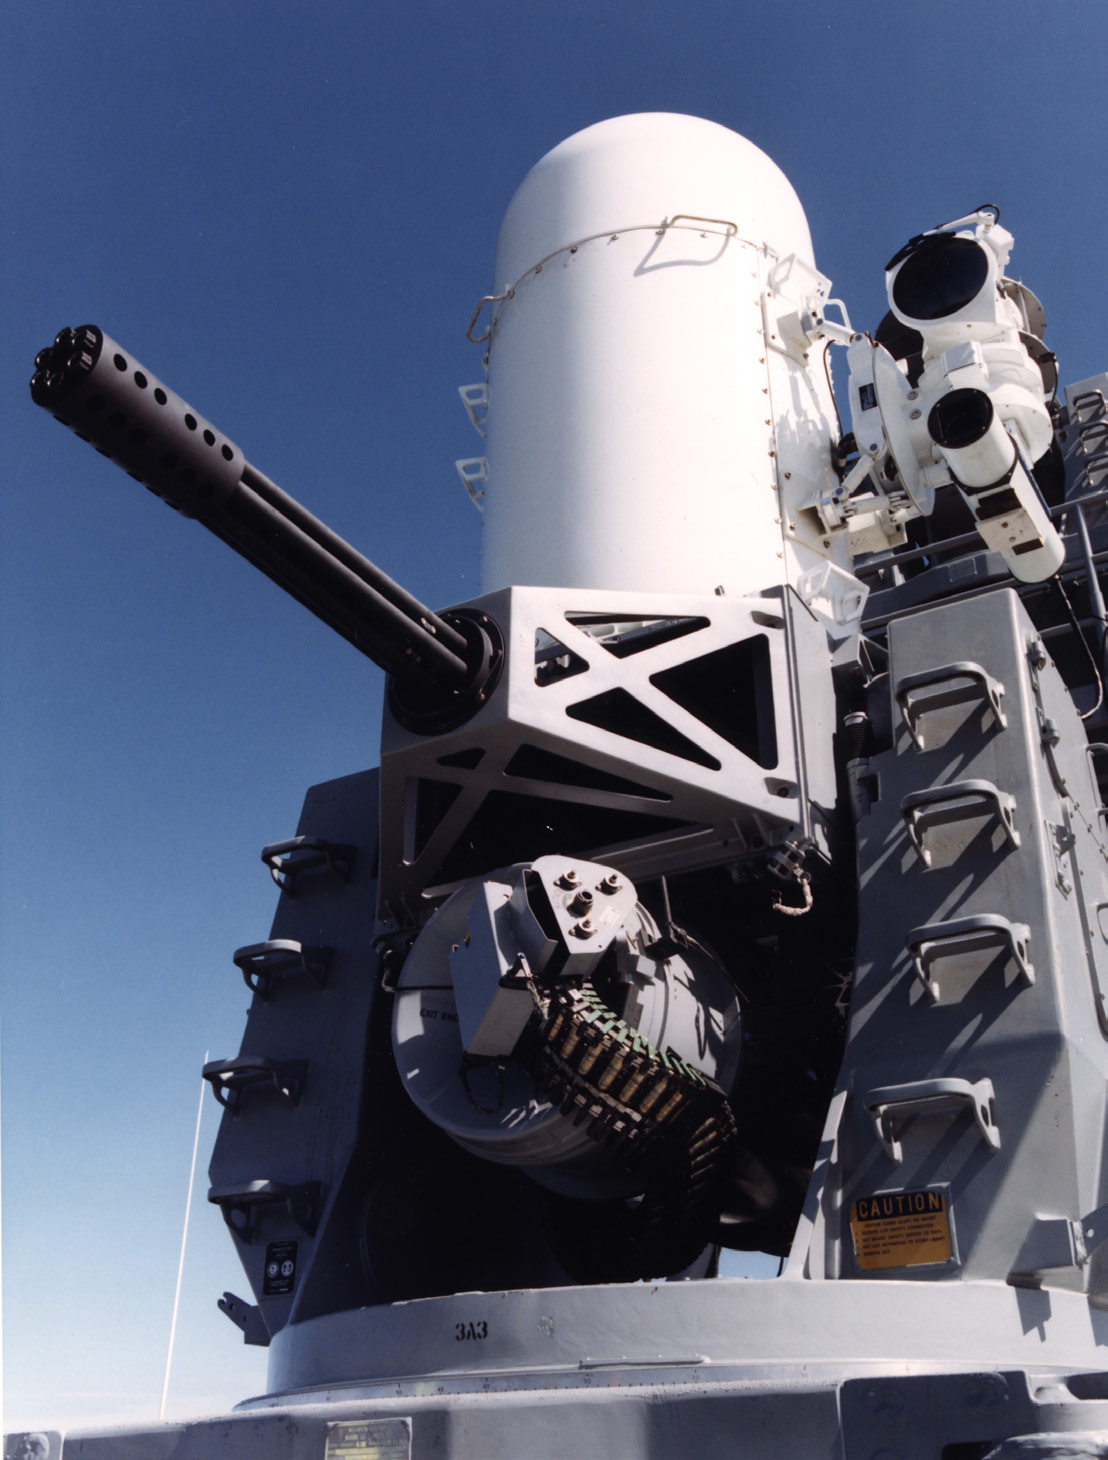
\includegraphics[width=.45\linewidth]{irod_phalanx} 
	\caption{Phalanx CIWS rendszer \cite{CIWS}}
	\label{fig:irod_phalanx}
\end{figure}

Mint manapság az ipar minden területén, így a fegyveriparban is egyre nagyobb mértékű a digitalizáció és az automatizáció. Ennek ékes példája a távolról irányítható lőállások térnyerése, amelyeknek nagy előnye a fegyver és a tüzér egymástól való elkülönítése, aminek több előnye is van. Természetesen a legfontosabb és leginkább szembetűnő, hogy ezzel a módszerrel minimalizálható, vagy akár megszüntethető a saját embereink életének kockáztatása. Ezentúl olyan helyen is tudjuk használni ezeket az eszközöket, ahova egy tradicionális géppuskafészek telepítése nehézkes lenne, például mostoha természeti körülmények közé, egy torony tetejére, vagy akár egy hadihajó oldalára. Szintén egy nagy előny, hogy ezek az eszközök felszerelhetők több kezeléssegítő alegységgel, például hőkamerával vagy éjjellátóval. Majdnem minden, számottevő hadsereggel rendelkező országnak van saját fejlesztésű távirányított fegyverrendszere.\\


A következő lépés az automatizálás. Hiszen egyre erősebb hardverekkel rendelkezünk, egyre jobb algoritmusokat tudunk implementálni, és elértük az a szintet, hogy bizonyos helyzetekben a "gép" jobb munkát tud végezni, mint egy ember. Az első automatikus célzórendszerrel rendelkező légvédelmi gépágyú az amerikai \textsl{Phalanx CIWS} \cite{CIWS} az 1970-es években került kifejlesztésre, ezzel megszületett a "Lethal autonomous weapon (LAW)" kifejezés.\\

A technológiát érthető módon leggyakrabban védelmi célokra használják, sokszor légvédelemre. A gyakorlatban nagy szerepe van Dél-Korea és Izrael védelmében, ahol a rakétatámadások mindennapos veszélyt jelentenek. Offenzív célokra a gyakorlatban még csak rakéták célzására használnak automatikát, a "terminátor" jellegű gyilkos robotok még csak fejlesztési fázisban vannak.


\section{Kihívások és célkitűzések}

A hagyományos, ember által irányított biztonsági rendszerek, illetve manuálisan vezérelt fegyverek hatékonysága korlátozott. Az ember reakcióideje lassú lehet krízishelyzetben, különösen ha nagy sebességű, gyors reagálású, esetleg automatizált a célpont. További gyengesége az embernek, hogy hajlamos hibázni. A fáradtság, stressz, éhség, és rengeteg egyéb tényező kényszerítheti hibára. Ez szükségessé teszi egy olyan automata rendszer kifejlesztését, amely képes azonnal reagálni, felismerni a fenyegetéseket és pontosan célozni.\\

Az automatikus gépágyúk fejlesztése során számos technikai kihívás merül fel:\\

\textbf{Célpontok felismerése és követése:} A gépágyúnak gyorsan és pontosan kell érzékelnie és nyomon követnie mozgó célpontokat. Ez kihívást jelenthet változó fényviszonyok, mozgássebességek és környezeti zavaró tényezők mellett. A gépágyúnak gyorsan és pontosan kell érzékelnie és nyomon követnie mozgó célpontokat. Ez kihívást jelenthet változó fényviszonyok, mozgássebességek és környezeti zavaró tényezők mellett. \\

\textbf{Pontosság és reakcióidő:} A rendszernek gyorsan kell döntéseket hoznia, ugyanakkor elengedhetetlen a pontos célzás. A mechanikai mozgásvezérlés, a számítógépes látás és az elektronikai rendszerek szinkronizációja mind kritikus tényező a rendszer hatékonysága szempontjából. \\

\textbf{Környezetérzékenység:} Külső környezeti tényezők (pl. időjárás, akadályok, fényviszonyok) befolyásolhatják a rendszer működését, ezért a szoftvernek és a hardvernek rugalmasnak és robusztusnak kell lennie. A dolgozatom célja egy innovatív megoldás kidolgozása, amely eleget tesz a megszabott követelményeknek és megoldást nyújt a fenti problémákra. \\


Kiemelt célok:
\begin{list}{}{}
	\item Egy megbízható célpontfelismerési rendszer fejlesztése, amely változó környezeti feltételek mellett is képes hatékonyan működni.
	\item Egy stabil és erős mechanikai konstrukció tervezése, amely képes képes követni a szoftver utasításait.
	\item Egy olyan valós idejű szoftvervezérlési rendszer megalkotása, amely gyorsan reagál a célpontok mozgására és változására.
\end{list}

Összegezve tehát: \\

\textbf{Egy olyan automata gépágyú fejlesztése és megépítése, amely magabiztosan képes felismerni egy célpontot, követni azt, célozni, és tüzelni.}

\section{Korlátozások}

Természetesen tisztában kell lenni bizonyos korlátozásokkal a projekt elkészítése közben. Két félévem van lefejleszteni az eszközt a nulláról, egyedül vagyok, és nincsen százmilliós büdzsém, mint az iparban hasonló kutatással foglalkozó csapatoknak. Ebből kifolyólag reálisan kell látni a helyzetet, és úgy meghatározni a követelményeket, hogy egy egyetemi hallgató számára is elérhető legyen. \\

A kamerarendszer például, amit a valós megoldásokban használnak, önmagában tízmilliós tétel szokott lenni. Sajnos az én megvalósításom valószínűleg nem fog működni sötétben, nagy távolságokban, vagy esőben, hiszen a költségvetésbe nem fér bele az éjjellátó, a hőkamera, az optikai zoom vagy több kamerából álló rendszer.\\

Nem áll rendelkezésemre korlátlanul se CNC gép, se fém 3D nyomtató, így a legtöbb alkatrész műanyagból kell 3D nyomtatnom. Ez befolyásolhatja a szerkezet stabilitását, amit figyelembe kell venni a későbbiekben.\\

És végül fontos megemlíteni, hogy mivel éles fegyvert alkalmazni minden bizonnyal a törvénybe ütközne, ezért valamilyen játékfegyvert kell majd használnom. Ez befolyásolni fogja a gépágyú pontosságát, amit szintén figyelembe kell venni a tervezéskor és értékeléskor.\\


\pagebreak

\section{Erkölcsi nyilatkozat}
Az automata fegyverrendszer morális megítélése vitatott téma, ezért szeretném kijelenteni, hogy diplomamunkám, melynek címe \textsl{„Mikrovezérlő alapú autonóm fegyverrendszer tervezése és fejlesztése”}, kizárólag tanulányni és mérnöki célokat szolgál. A dolgozatom keretében fejlesztett prototípus semmilyen formában nem szándékozik vagy ösztönzi az erőszakos, káros vagy törvénysértő tevékenységeket. Fejlesztésem célja a technológiai kutatás, a mechatronikai és automatizálási rendszerek megismerése, illetve a gépi látás alkalmazásainak tanulmányozása. \\

Határozottan elhatárolódom bármilyen rosszindulatú felhasználástól, és hangsúlyozom, hogy a projekt eredményei nem használhatók fel ártalmas vagy illegális célokra. A munka során mindvégig tiszteletben tartottam az etikai irányelveket, és felelős mérnöki magatartást tanúsítottam. Az általam fejlesztett rendszer kizárólag oktatási, kutatási és technológiai demonstráció célját szolgálja.

%----------------------------------------------------------------------------
\chapter{Irodalomkutatás}
%----------------------------------------------------------------------------

A legjelentősebb katonai hatalmak mindegyike rendelkezik távvezérelt fegyverrendszerekkel, leggyakrabban valamilyen távolról irányított gépfegyver formájában. Azonban se az egyes országok nemzetbiztonságának, se a fegyveripari partnercégeknek nem áll érdekében a szükségesnél több információt kiadni. Ez egy kicsit megnehezítette az irodalomkutatást, de a képek alapján azért sok információt ki lehet nyerni.

\section{Megvalósult rendszerek} \label{sec:valos}

\subsubsection*{CROWS}
Az egyik legnagyobb darabszámban gyártott távirányított fegyverrendszer az amerikai \textsl{CROWS} \cite{crows} rendszer, amely a NATO-országokban, köztük Magyarországon is rendszeresített. Ennek értelmében telepíthető sok NATO által használt páncélozott járműre, köztük a \textsl{Humvee}-ra, a \textsl{Stryker}-re, és a \textsl{Buffalo MRAP}-re. Több verziója létezik több kaliberrel, a \ref{fig:irod_crows}. ábrán egy \textsl{M240B} géppuskával látható.\\

\begin{figure}[h!]
	\centering
	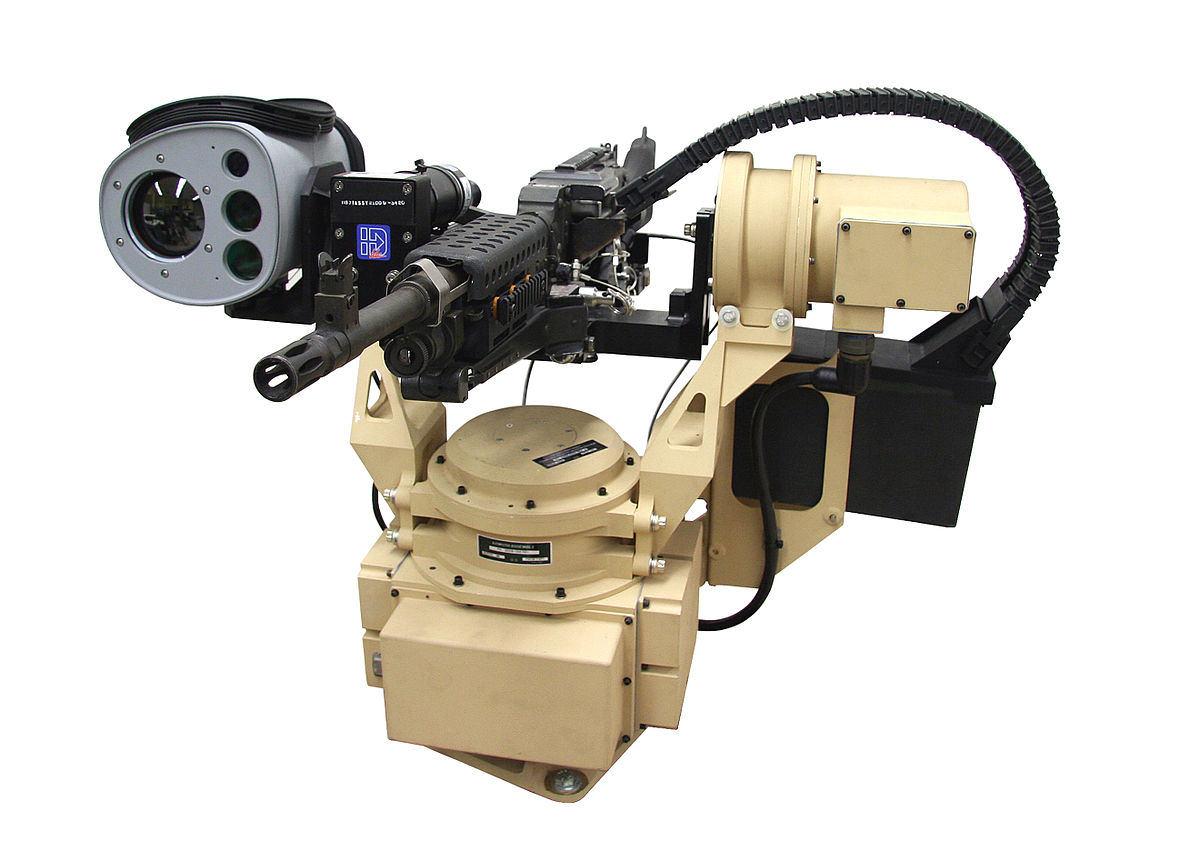
\includegraphics[width=.7\linewidth]{irod_crows}
	\caption{Az amerikai CROWS rendszer \cite{crows}}
	\label{fig:irod_crows}
\end{figure}

A szerelék a fegyverrel együtt $360^\circ$-ban képes elfordulni, és $-20^{\circ}$-tól $+60^{\circ}$-ig tud billenni. A fegyvercső giroszkóppal stabilizált. A kezelő egy 15 hüvelykes kijelzőn tud célozni a fegyverrel. A rendszer a sima kamera mellett rendelkezik hőkamerával is, így éjszaka is használható. Mind a két kamera el van látva lézeres távolságmérővel, amivel rá lehet állni a célpontra, és a jármű mozgása közben is lehet azt követni. A kamerát és a fegyvert lehet külön is mozgatni, ami azért hasznos, mert anélkül lehet követni a gyanús alakok mozgását, hogy félelmet keltenénk az emberekben.

\subsubsection*{Arbalet-DM}
A \textsl{CROWS} rendszer orosz megfelelője a hasonló kialakítású \textsl{Arbalet-DM}  \cite{arbalet} (\ref{fig:irod_arbalet}.ábra). Ennek a rendszernek az alapja a 12.7 mm-es \textsl{KORD} nehézgéppuska. Rendelkezik 4 gránátvetővel is, amelyek füstfüggöny felhúzására használható. A kamera és a fegyver elhelyezése, de még a lőszer pozíciója is teljesen hasonló az amerikai párjához.

\begin{figure}[h!]
	\centering
	\includegraphics[width=.7\linewidth]{irod_arbalet}
	\caption{Az orosz Arbalet-DM rendszer \cite{arbalet}}
	\label{fig:irod_arbalet}
\end{figure}

A rendszer $360^\circ$-ban képes elfordulni, és $-20^{\circ}$-tól $+70^{\circ}$-ig tud billenni, tehát egy kicsit nagyobb részt tud lefedni, mint a CROWS. A hatótáv nappal 2000 m, éjszaka 1500 m. Ez a rendszer is el van látva hőkamerával és lézeres távolságmérővel.

\subsubsection*{DeFNder}
A következő megoldás a belga \textsl{DeFNder} \cite{defnder} termékcsalád, amelynek két tagja a \textsl{Light} és a \textsl{Medium}(\ref{fig:irod_defnder}. ábra). Értelem szerűen kettő közül az utóbbi az, amelyre nehezebb fegyverzetet lehet telepíteni. A függőleges tengelyen $360^\circ$-ban képes elfordulni 90 fok/másodperc sebességgel, a vízszintes tengelyen $-45^{\circ}$-tól $+75^{\circ}$-ig tud billenni, 60 fok/másodperc sebességgel. Opcionálisan ellátható infravörös- és hőkamerával a rossz látási körülmények esetére, valamint lézeres távolságmérővel a ballisztikai kompenzációhoz.
\begin{figure}[h!]
	\centering
	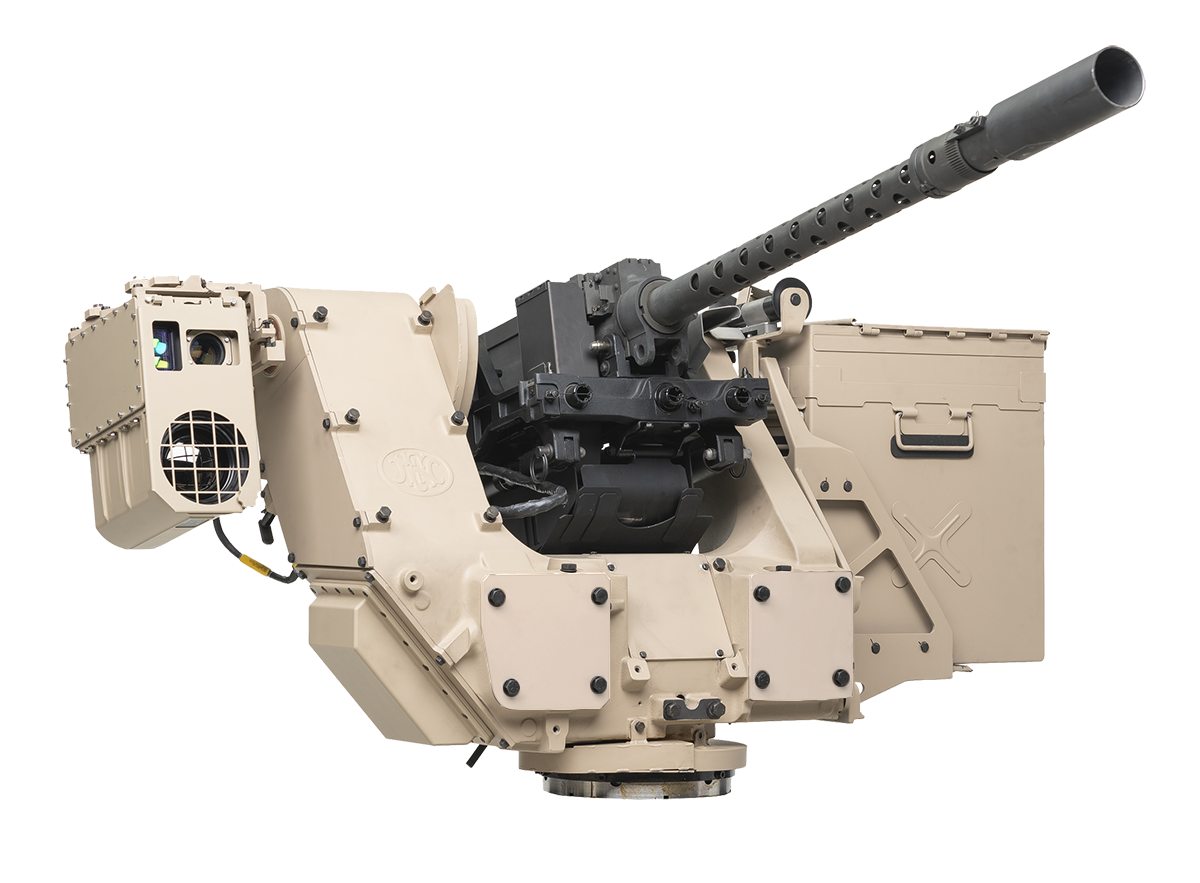
\includegraphics[width=.6\linewidth]{irod_defnder}
	\caption{A belga DeFNder rendszer \cite{defnder}}
	\label{fig:irod_defnder}
\end{figure}

Elég sok közös vonást találtam a fentebb említett rendszerekben. Az elrendezésük nagyon hasonló, van egy függőleges forgástengely nagyjából a teljes rendszer súlypontján keresztül, valamint egy vízszintes forgástengely, nagyjából a fegyver csövével egy síkban. Erre valószínűleg azért van szükség, hogy a tüzelés során keletkező erők ne ébresszenek csavarónyomatékot a mozgató mechanizmuson. Az én esetemben nagy erők nem fognak ébredni, de a tervezési elvet érdemes követni.

\subsubsection*{Samsung SGR-A1}
Az egyetlen, valós harci helyzetben használt, teljesen autonóm gépágyú a koreai fejlesztésű \textsl{Samsung SGR-A1}  \cite{samsung}. A két Korea között húzódó demilitarizált övezet (DMZ) egy 250 km hosszú, 4 km széles sáv, amelyet mind a két oldalon szigorúan ellenőriznek. A határ folyamatos felügyelete rengeteg ember munkájába kerül, ami egy demográfiai válságban lévő ország csökkenő hadseregében egyre értékesebb. Főleg annak tekintetében, hogy csupán járőrözni és figyelni a határt nem feltétlenül igényli egy ember jelenlétét. Ennek tudatában fejlesztették ki a Samsung és a Korea Egyetem mérnökei az SGR-A1 fegyverrendszert. Hőkamerával és éjjellátóval felszerelve napközben 4 km-ről, éjszaka 2 km-ről képes azonosítani potenciális célpontokat, tehát tulajdonképpen a DMZ teljes szélességében. Képes felismerni az embereket, követni őket, és megkülönböztetni más élőlényektől. Hangfelismeréssel képes azonosítani a közeledő személyeket: amennyiben valaki 10 m-nél közelebb kerül és nem azonosítja magát, a rendszer riaszthat, gumilövedéket lőhet, vagy használhatja a K-3 gépfegyverét.

\begin{figure}[h!]
	\centering
	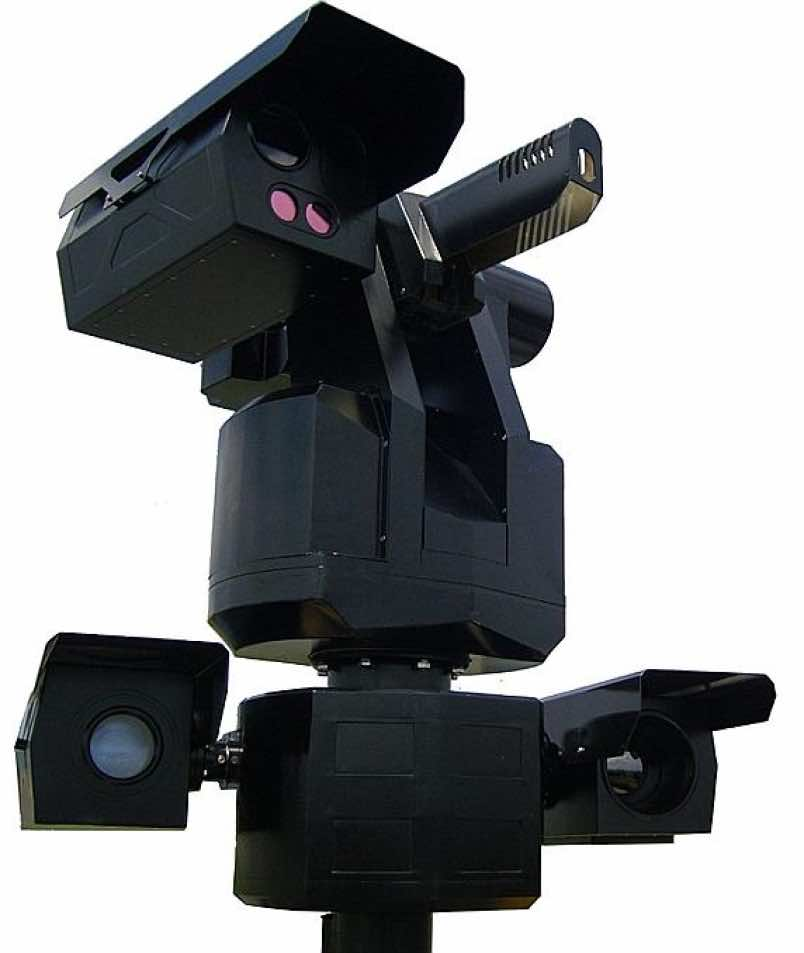
\includegraphics[width=0.35\linewidth]{irod_samsung}
	\caption{Samsung SGR-A1 \cite{samsung}}
	\label{fig:irod_samsung}
\end{figure}

Civil szakértők számára nem egyértelmű, hogy a rendszer lőhet-e emberi engedély nélkül, és a hivatalos koreai álláspont az, hogy nem. Azonban ha már bemérte és ellenségként azonosította a célpontot, akkor nehéz elképzelni, hogy pont a ravaszt ne tudná meghúzni.

\pagebreak

\section{Tüzelési mechanizmus}

A korábban említett rendszerek éles fegyverekkel vannak felszerelve, amit természetesen nem fogok követni. Így valamilyen olyan megoldást kellett találni, ami legális, elegendően pontos és megfelelően be lehet vele mutatni a célfelismerés és célzás működését. 


\subsubsection*{Paintball}

Több, a diplomamunkámhoz hasonló projektet is találtam, amelyek \textsl{paintball}  \cite{paintball} puskákat használnak. Ezek a puskák sűrített levegőt alkalmaznak, hogy egy festékkel töltött golyót lőjenek ki. A torkolati sebességük nagyjából 280 fps, maximális hatékony távolságuk kb 25-30 m. Mivel a lövedék alakja gömb, és a cső sincs huzagolva, ezért nem túl pontos, főleg hosszú távon.\\

\begin{figure}[h!]
	\centering
	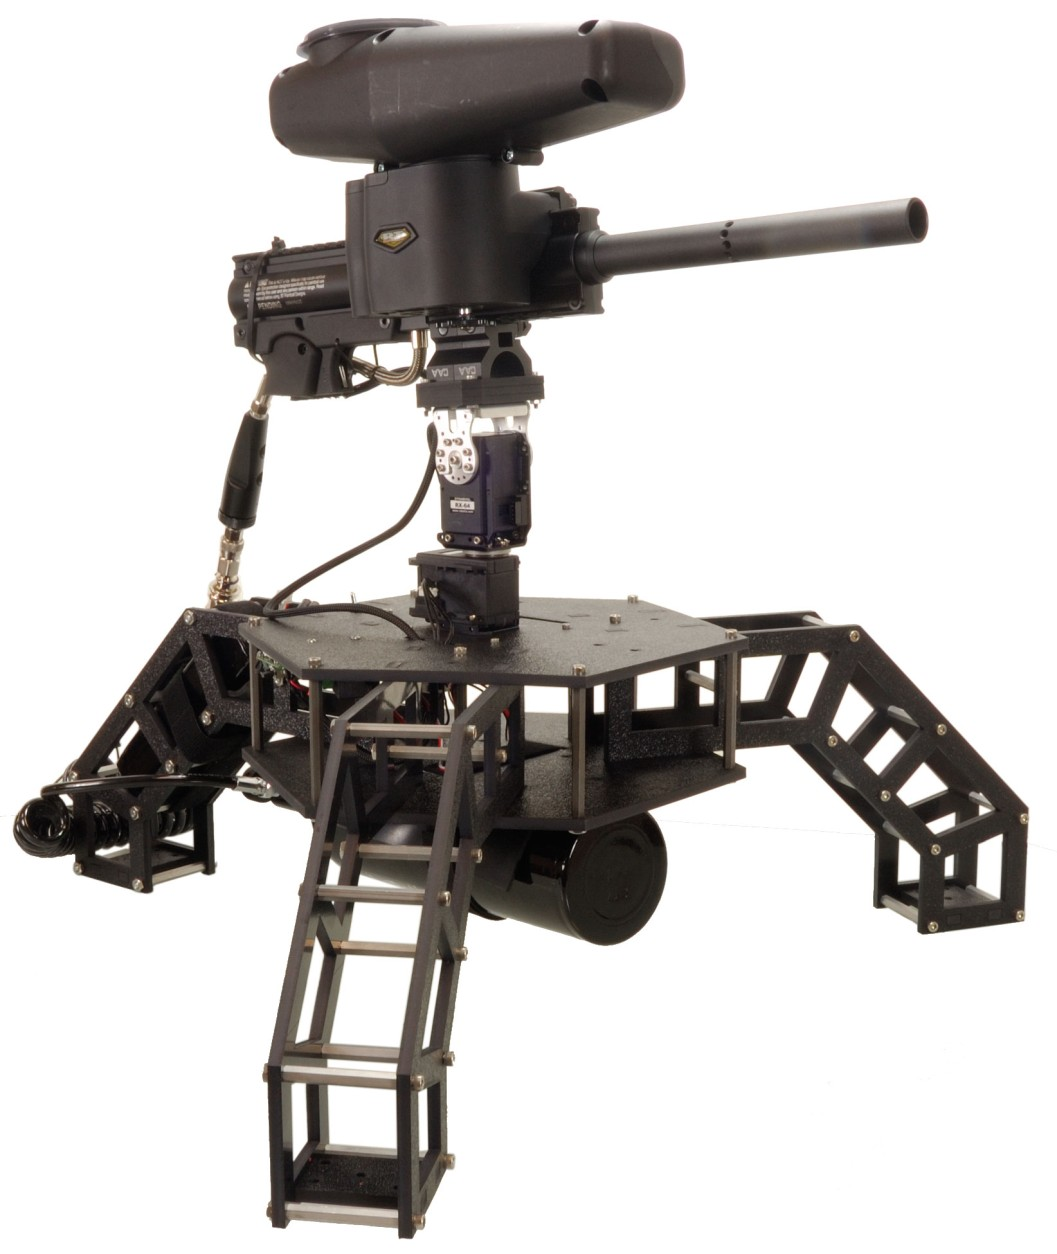
\includegraphics[width=0.4\linewidth]{irod_paintball}
	\caption{Paintball puska alapú rendszer \cite{paintballrobot}}
	\label{fig:irod_paintball}
\end{figure}

További problémák, hogy a legolcsóbb paintball puska is 70000 Ft. fölött van, valamint a lövedék is viszonylag drága, és nem lehet újrahasznosítani. Ezentúl a fegyverek nagyok, nehezek, és ezért nehéz a beépítésük. 


\subsubsection*{Nerf}

A \textsl{Nerf} \cite{nerf} fegyverek a legelterjedtebb játékfegyverek. Sűrített levegővel lőnek ki egy hosszúkás szivacs lövedéket. A sűrített levegőt egy megfeszített rugó elengedésével érik el, amelyet vagy kézzel, vagy valamilyen áttételes villanymotorral húznak fel. A legjobb modellek torkolati sebessége 70 fps körül van, és kb. 15 m a hatótávolságuk. Ezen a távon viszonylag pontosak a lövedék kialakításából adódóan, de jelentős az esés, így a ballisztikai pályát komolyan kell venni. \\

Ezek a fegyverek modelltől függően 10000 Ft. - 40000 Ft. között mozognak, de a lövedékeket újra lehet használni. Az a probléma itt is fennáll, hogy nagy a fegyver teste, így nehezebb beépíteni. 

\subsubsection*{Airsoft}

Az \textsl{airsoft} \cite{airsoft} fegyverek hasonló módon működnek, mint a \textsl{Nerf} puskák, de egy kisebb, műanyag golyót lőnek. Az elektromos airsoft fegyverek torkolati sebessége általában 300 fps és 400 fps között van, ami befolyásol a golyók tömege, a rugó minősége és rengeteg egyéb alkatrész. A hatótávjuk az átlagos fegyvereknek kb. 50 m, de fejlesztésekkel elérheti a 90 m-t is. A lövedék itt is golyó és a cső sincs huzagolva, mint a paintballnál, azonban az airsoft esetében használnak ún. hop-up kamrákat, amelyek perdületet adnak a golyónak.\\

Az airsoft fegyverek legnagyobb előnye a többi lehetőséggel szemben, hogy van egy kompakt egység, a "gearbox", ami felelős az elsütésért. Ezt ki lehet szedni egy fegyverből, vagy akár külön is meg lehet venni. Ez okkal nagyobb szabadságot ad a beépítéshez, és a végeredmény is sokkal kompaktabb lesz. Az elsütés is csak az áramkör zárását jelenti a gearboxban, ami egyszerűen vezérelhető a mikrokontrollerrel.
\chapter{Rendszertervezés és követelmények}

\section{Rendszeráttekintés}
Az autonóm fegyverrendszer fejlesztése során egy komplex mechatronikai rendszert kellett megvalósítani, amely több különálló modul együttműködését biztosítja. A rendszer fő komponensei közé tartozik a mechanikai szerkezet, az elektronikai hardver, az érzékelők, a vezérlő egység, valamint a szoftveres háttér. Ezek együttesen biztosítják a rendszer autonóm és manuális működését. Az alábbiakban részletes áttekintést adok a rendszer főbb elemeiről és azok feladatáról.

\subsubsection*{Mechanikai konstrukció}

A váz gyanánt tulajdonképpen egy kéttengelyes pan-tilt mechanizmust kellett megvalósítanom, ami felelős a fegyver stabilan tartásáért és precíz mozgásáért. A váz építőelemei zömében 3D nyomtatási technológiával készültek, ami lehetővé tette a problémák gyors kiküszöbölését, illetve a nagyfokú szabadságot a tervezés során. Ahol tudtam, kereskedelemből beszerezhető alkatrészeket használtam, például a csapágyakat és a kötőelemeket.\\

A modellt több alegységre lehet bontani a funkciójuk szerint. Van a \textsl{torony} nevezetű alösszeállítás, amely feladata a gearbox stabil befogása, illetve erre épül rá a kamera konzolja, a tár összeállítása, a fogaskerék és a lézer is. A következő a \textsl{keret}, amelybe kerülnek a torony csapágyai, illetve az elektonika egy része. Erre az elemre van erősítve a Raspberry Pi konzolja, a relé, illetve az egyik motor is. A torony alatt található a \textsl{nagy csapágyhoz }tartozó elemek, amelyeknek feladata a stabil összeköttetés biztosítása a keret és a talp között. Legalul helyet kapott a \textsl{talp}, amely magába foglalja a lábakat, illetve az azokat összefogó elem is. Ezt úgy terveztem, hogy a lábak szükség esetén cserélhetőek legyenek.

\pagebreak
\subsubsection*{Elektronikai rendszer}
Az elektronikai rendszer blokkdiagrammja a \ref{fig:system_blokkdiagram}. ábrán látható.\\

\begin{figure}[h!]
	\centering
	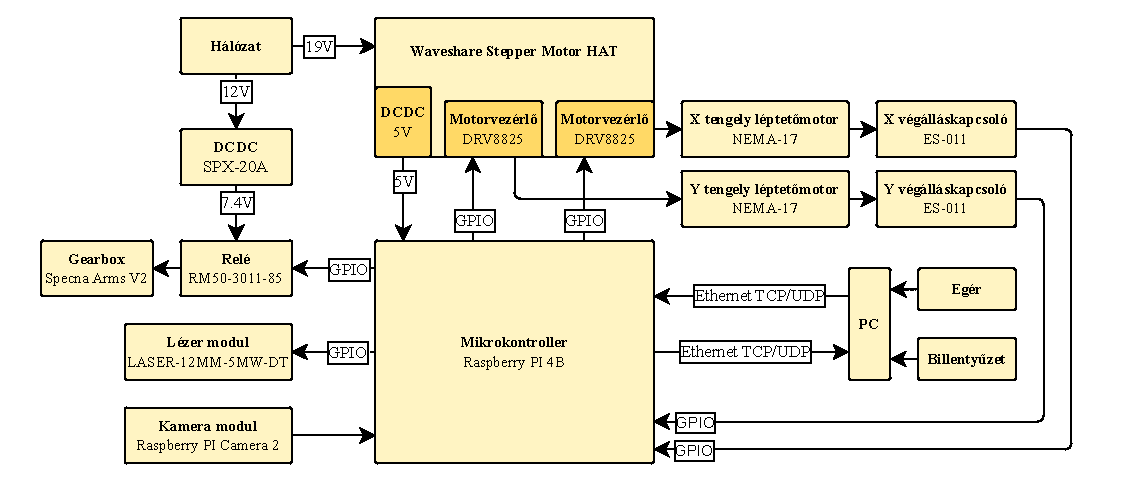
\includegraphics[width=1\linewidth]{blokkdiagram_vegleges}
	\caption{Az elektronikai rendszer blokkdiagrammja}
	\label{fig:system_blokkdiagram}
\end{figure}

Az elektronikai rendszer két fő eleme a Raspberry Pi, illetve a gearbox volt. Mivel a gearbox igen nagy áramot képes felvenni, külön tápegységgel kellett ellátnom a mikrovezérlőt illetve a golyó kilövéséért felelős elektronikát. A motorok vezérléséért egy kereskedelemben kapható, Raspberryvel kompatibilis shieldet használtam, amely jelentősen megkönnyítette a NEMA-17 típusú léptetőmotorok csatlakoztatását. A lézer diódát és szükséges szenzorokat a Raspberry Pi GPIO lábairól vezéreltem, ahogy a gearbox aktiválásáért felelős relét is. A kamera modul egy Raspberry Pi Camera V2 volt, amit a mikrovezérlőn található foglalaton keresztül tudtam elérni. 

Az elektronika központi egysége természetesen a \textsl{Raspberry Pi} mikrokontroller volt, amely felelős volt a fő képfelismerő algoritmus futtatásáért, a szenzorok jeleinek feldolgozásáért, valamint a PC-vel való kommunikációért. A mikrokontroller kiegészült egy \textsl{Stepper Motor HAT}-el, amely egy kereskedelemben kapható áramkör. Megtalálható rajta két db. \textsl{DRV8825} motorvezérlő chip, illetve kiegészítő áramkörök, pl. microstep állító kapcsolók, valamint áramkorlátozó potméterek. Ezentúl helyet kapott egy 5V-os DCDC konverter, amin keresztül a Raspberry Pi-t is elláthatjuk árammal. A léptetőmotorok \textsl{NEMA-17} típusúak, és 4 tüskés csatlakozóval rendelkeznek.\\

Az elektronikai rendszerben szerepel még a \textsl{gearbox}, ami a tüzelésért felel. Mivel igen nagy áramot képes felvenni, ezért külön áramellátást terveztem a gearboxnak. Egy 12V-os szervertáp működteti, amiből egy \textsl{SPX-20A} típusú, nagy teljesítményű DCDC konverter csinál a gearbox számára optimális 7.4V-ot. Ez a kimeneti feszültség állítható, a gearbox egészen 11V-ig képes működni. A kimeneti feszültséggel tulajdonképpen a tüzelés sebességét tudjuk szabályozni. A gearbox áramellátását egy relével lehet vezérelni, amely a Raspberry Pi GPIO lábára csatlakozik.

\pagebreak

A rendszerben helyet kapott mindkét tengelyre 1-1 \textsl{végálláskapcsoló}, amelyek a fegyver kalibrálásáért felelősek. Ezek a GPIO tüskesoron csatlakoznak a mikrovezérlőhöz. Hasonlóképpen a \textsl{lézer dióda} is, amely a fegyver célzásával hivatott segíteni a felhasználót. A RAspberry Pi kamera csatlakozóján keresztül pedig beépítésre került egy \textsl{Raspberry Pi Camera 2} típusú kamera. A mikrovezérlő a rajta található \textsl{Ethernet} porton keresztül kommunikál a PC-vel.

\subsubsection*{Számítógépes vezérlés és szoftveres háttér}
A szoftver rendszere két alegységből áll, a Raspberry Pi-n \textbf{beágyazott vezérlő szoftverből}, illetve a PC-n futó \textbf{felhasználói alkalmazásból}. Mivel magát a prototípust szeretném minél jobban közelíteni a valósidejű működéshez, ezért a két alegység közötti kommunikáció sebessége kiemelkedően fontos. Ezért döntöttem úgy, hogy a Raspberry Pi az Ethernet portján keresztül csatlakozzon a PC-hez. Ez ugyan kissé megköti a fegyver mozgásterét, de nem annyira, hogy feláldozzam a kapcsolat gyorsaságát. \\

A Raspberry Pi-n futó szoftver felelős a léptetőmotorok mozgatásáért, a felhasználó parancsainak fogadásáért, a célpont felismeréséért, illetve a  kamera képének továbbításáért a PC felé. Ezeket a folyamatokat jól elkülönülő modulokra bontottam, amelyek egyszerre futnak külön szálakon. A különböző folyamatok közötti kommunikációra használtam megosztott erőforrásokat, állapotjelzőket és queue-kat. A kézi vezérlés és az automata működés között is tettem különbséget, a szoftver bizonyos részei között is megosztott változókkal lehet választani. \\

A PC-n futó szoftver felelős a Raspberry által küldött videó dekódolására, és megjelenítésére a \textsl{HUD}-on. A HUD-on szerepelnek még fontos állapotjelzők, pl. hogy éppen melyik működési módban van a rendszer, vagy hogy be van-e biztosítva a fegyver. Emellett A szoftvernek fel kell dolgozni a felhasználótól kapott parancsokat is, és tovább kel küldenie a Raspberry Pi felé. Ez a program is két külön szálon futó alegységből áll, amelyek megosztott erőforrásokkal kommunikálnak egymással. 

\pagebreak

\section{Követelmények}\label{sec:kov}


Az autonóm fegyverrendszer fejlesztése során számos követelményt kellett figyelembe venni annak érdekében, hogy a rendszer megbízhatóan, hatékonyan és biztonságosan működjön. Ezek a követelmények a rendszer mechanikai, elektronikai és szoftveres elemeire egyaránt kiterjedtek. A következő szakaszokban részletezem a legfontosabb műszaki és funkcionális követelményeket.

\subsubsection*{Mechanikai követelmények} 

A mechanikai komponensek tervezése során az alábbi követelményeknek kellett megfelelni:
\begin{list}{}{}
	\item \textbf{Stabilitás és pontosság:}  A fegyverrendszer mechanikai szerkezetének stabilnak és tartósnak kell lennie annak érdekében, hogy a lövések közben ne mozduljon el, és ne veszítse el a célpontot. Ugyanakkor elegendő pontosságot kell biztosítania a célpont precíz követéséhez.
	\item \textbf{Fürgeség:} A rendszernek képesnek kell lennie a fegyver gyors és pontos mozgatására a pan-tilt mechanizmus segítségével. Ennek megfelelően a szervomotoroknak kellően gyorsnak és erősnek kell lenniük ahhoz, hogy valós időben tudják követni a mozgó célpontokat.
	\item \textbf{Strapabíró konstrukció:} Habár nagy terhelés nem fogja érni, a gearboxból jöhetnek rezgések, rángások, amik esetleg problémát jelenthetnek egy alulméretezett alkatrész esetében.
\end{list}

\subsubsection*{Elektronikai követelmények}

Az elektronikai rendszer megbízható működése érdekében az alábbi követelményeknek kellett eleget tenni:

\begin{list}{}{}
	\item \textbf{Megfelelő teljesítmény:}  A szervomotoroknak és szenzoroknak megfelelő tápegységre van szükségük, amely stabil energiaellátást biztosít. A rendszer energiaigényét előzetesen fel kellett mérni, hogy a tápegység terhelés alatt is megfelelően működjön.
	\item \textbf{Szenzorok pontossága:} A kamerának és egyéb szenzoroknak elegendő felbontással és érzékenységgel kell rendelkezniük ahhoz, hogy képesek legyenek a célpontokat megfelelően azonosítani. A valós idejű képfeldolgozás nagy adatsebességet és megbízható szenzorjeleket igényel.
	\item \textbf{Vezérlés:} A mikrokontrollernek kellően gyorsnak kell lennie, hogy a valós idejű adatokat folyamatosan feldolgozza és a vezérlési parancsokat késlekedés nélkül végrehajtsa.
\end{list}
\pagebreak

\subsubsection*{Szoftveres követelmények}

A rendszer működéséhez szükséges szoftverfejlesztés során a következő követelményeknek kellett megfelelni:

\begin{list}{}{}
	\item \textbf{Valós idejű feldolgozás:}  A számítógépes látás szoftverének valós időben kell elemeznie a kamerák által közvetített adatokat, felismerve a célpontokat és kiszámítva a mozgás irányát. A célzási és lövési döntések gyors és hatékony adatfeldolgozást igényelnek.
	\item \textbf{Biztonságos működés:} A rendszernek rendelkeznie kell olyan szoftveres biztonsági funkciókkal, amelyek megakadályozzák a véletlen tüzelést. Ez magában foglalja a lövési engedélykérés mechanizmusát és a manuális vészleállítás lehetőségét.
	\item \textbf{Felhasználói interfész:} Az felhasználónak egyszerű és intuitív felhasználói felületet kellett biztosítani, amelyen keresztül könnyedén vezérelheti a rendszert, illetve áttekintheti a célpontok adatait és a kamera képét. A felületnek támogatnia kell a kézi irányítást és a lövési parancsok kiadását.
\end{list}




\subsubsection*{Funkcionális követelmények}

A rendszer teljes funkcionalitásának biztosítása érdekében a következő kritériumoknak kellett megfelelni:

\begin{list}{}{}
	\item \textbf{Autonóm működés:} A rendszernek képesnek kell lennie arra, hogy teljesen önállóan felismerje és kövesse a célpontokat, valamint meghozza a tüzelési döntéseket az előre meghatározott paraméterek alapján.
	\item \textbf{Manuális vezérlés:} Az autonóm működés mellett manuális vezérlési lehetőséget is kellett biztosítani az operátor számára. Ezen keresztül a felhasználó közvetlenül irányíthatja a fegyvert és manuálisan adhat lövési parancsot.
\end{list}

\subsubsection*{Biztonsági követelmények}

Az autonóm fegyverrendszerek használatával kapcsolatban különösen fontos a biztonsági követelmények teljesítése:

\begin{list}{}{}
	\item \textbf{Vészleállítás:} A rendszernek rendelkeznie kell egy vészleállító gombbal, amely azonnal megszakítja a fegyver működését, ha bármilyen hiba vagy vészhelyzet lép fel.
	\item \textbf{Engedélyezési mechanizmus:} A tüzelési parancs kiadása előtt a rendszernek engedélyt kell kérnie az operátortól, ezzel minimalizálva a véletlen tüzelés kockázatát.
	\item \textbf{Adatbiztonság:} A vezérlő szoftver és az operátor közötti kommunikáció titkosítva kell, hogy legyen, hogy megakadályozza a külső hozzáférést és a rendszer kompromittálását.
\end{list}

\pagebreak

\subsubsection*{Környezeti követelmények}

A rendszernek különféle környezeti feltételek között is megbízhatóan kell működnie:

\begin{list}{}{}
	\item \textbf{Hőmérsékleti tűréshatár:}A rendszernek képesnek kell lennie normál működésre különböző hőmérsékleti körülmények között, amelyek tipikusan a beltéri használat során fordulnak elő.
	\item \textbf{Nedvesség és porállóság:} A rendszert úgy kell megtervezni, hogy ellenálljon a kisebb por- és nedvességterhelésnek, különösen, ha kültéri használatra is szükség van.
\end{list}

Azokhoz a követelményeket, amelyekhez tudok konkrét értéket rendelni, az alábbi táblázatban gyűjtöttem össze:

\begin{table}[ht]
	\footnotesize
	\centering
	\begin{tabular}{ c l c }
		\toprule
		\textbf{Nr.} & \textbf{Követelmény}                  & \textbf{Érték} \\
		\midrule
		1.           & Szögsebesség                          & 45°/ s \\
		2.           & Valósidejűség kézi vezérlésen         & 10 ms \\
		3.           & A célpont felismerése a képbe kerülés után    & 0.5 s \\
		4.           & Vízszintes tengely mozgási tartomány  & -10°\textless{}x\textless{}75°  \\
		5.           & Függőleges tengely mozgási tartomány  & -135°\textless{}y\textless{}135° \\
		6.           & Tüzelés pontossága 5m-en, 20cm x 20cm & 80\%                             \\
		7.           & Felhasználói felület felbontása       & 640x480                          \\
		8.           & Hőállóság                             & -10°C\textless{}T\textless{}50°C \\
		\bottomrule
	\end{tabular}
	\caption{Az órajel-generátor chip órajel-kimenetei.}
	\label{tab:TabularExample}
\end{table}
\chapter{Mechanikai tervezés}
A mechanikai tervezést egy kinematikai modell kidolgozásával kezdtem, majd a meglévő, kereskedelemben kapható alkatrészek méreteihez igazítva megterveztem a 3D CAD modellt. Ezután finomhangoltam a 3D nyomtatási technológiához megfelelően.
\section{Kinematika}
A rendszer kinematikai modellje hasonlatos a biztonsági kamerákhoz, aminek elnevezése Pan-Tilt-Zoom, röviden PTZ. Ennek lényege a 360 fokban elforgatható függőleges tengely, és egy általában korlátoltabb vízszintes tengely. Előnyük, hogy nagy sebességgel tudnak irányt változtatni, és nagy területet képesek belátni. A zoom aspektus az én esetemben nem fontos, hiszen nem a kamera a fő funkció. A \ref{fig:mech_pantilt}. ábrán erről látható illusztráció.

\begin{figure}[h!]
	\centering
	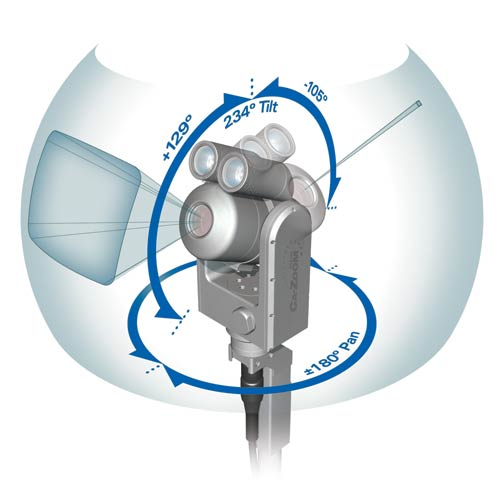
\includegraphics[width=0.6\linewidth]{mech_pantilt}
	\caption{PTZ kamera}
	\label{fig:mech_pantilt}
\end{figure}

A \ref{sec:valos}. bekezdésben vizsgált rendszerek is hasonlóképpen mozognak. Ezek közelebbi vizsgálata után elkezdtem kidolgozni a saját koncepciómat. Szemléltetésképpen készítettem a \ref{fig:megval_mockup}. ábrát. Az egyszerűség kedvéért a fegyver csövét egy síkba terveztem a pan és tilt tengelyekkel, ez megkönnyíti a későbbi számításokat.

\begin{figure}[h!]
	\centering
	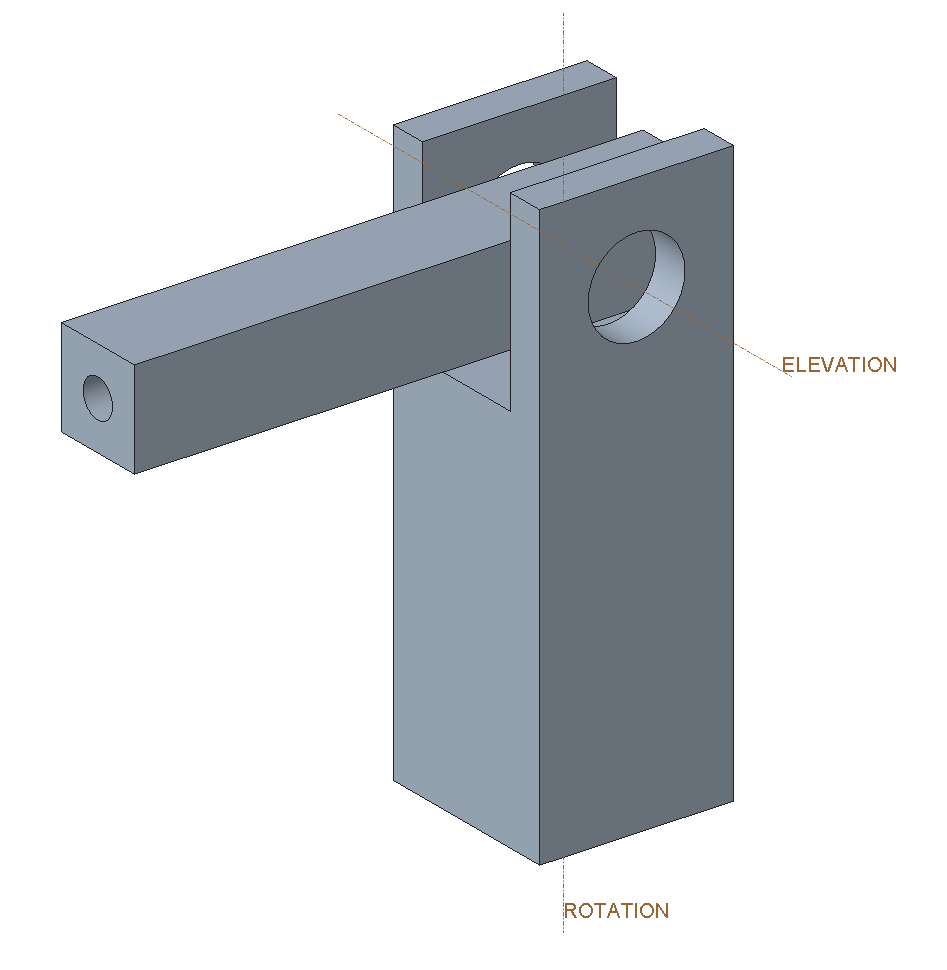
\includegraphics[width=0.6\linewidth]{mockup}
	\caption{Egyszerűsített kinematikai ábra}
	\label{fig:megval_mockup}
\end{figure}

Ki kellett számolnom bizonyos geometriai megkötéseket, amelyek szükségesek a tervezéshez, illetve az alkatrészek kiválasztásához. \\

A torony szükséges fordulatszámát a következőképpen lehet kiszámolni:


\begin{equation}
	rpm_{min} = \frac{v_t}{2 \cdot \pi \cdot r} = \frac{2.778 \w{m/s}}{2 \cdot \pi \cdot \w{m}} = 0.442 \w{1/s} = 26.526 \w{1/min}
\end{equation}

ahol:

\begin{tabular}{cl}
	$v_t$ & A célpont sebessége a fegyvercsőre merőlegesen, \\
	$r$ & A távolság a célpont és a rendszer között\\
\end{tabular}

Meg lehet állapítani a torony mozgásának felbontását is, tehát hogy hány fokonként lehet állítani a mozgását.

\begin{equation}
	\alpha_{min} = \arcsin\left(\frac{a}{2 \cdot r}\right) \cdot 2 = \arcsin\left(\frac{0.3 \w{m}}{2 \cdot 10 \w{m}}\right) \cdot 2 = 1.719 {^\circ}
\end{equation}

ahol:

\begin{tabular}{cl}
	$a$ & A célpont mérete  \\
	$r$ & A távolság a célpont és a rendszer között\\
\end{tabular}
\pagebreak
\section{Mechanikai alkatrészek}
\subsubsection*{Elsütő mechanizmus}
Az elsütő mechanizmusnak egy \textsl{Specna Arms M4}-ből kiszerelt gearbox-ot, illetve annak csövét és hop-up kamráját használtam. A gearbox működése során egy villanymotor több áttételen keresztül hátrahúz egy dugattyút, és azzal együtt a mögötte lévő rugót. Mindeközben a hop-up kamrában betöltődik egy golyó, és megáll a csőben. Ahogy a részlegesen fogazott fogaskerék elengedi a dugattyút, azt a rugó előrelöki, ezáltal a dugattyúkamrában nagy légnyomás keletkezik, ami a fegyver csövén keresztül tud kiegyenlítődni. Folyamatos működés során a motor egymás után húzza fel és engedi el a dugattyút, így amíg van golyó a tárban képes tüzelni. A gearbox belső alkatrészei a \ref{fig:mech_gearboxdiagram}. ábrán láthatóak. 

\begin{figure}[h!]
	\centering
	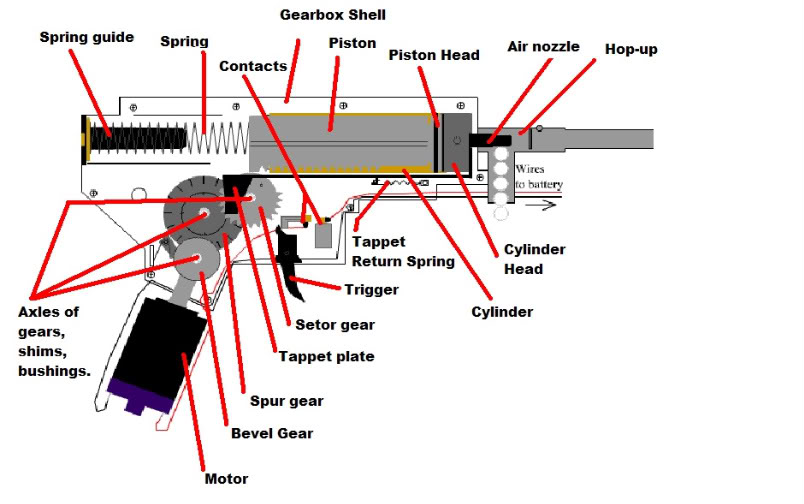
\includegraphics[width=1\linewidth]{mech_gearboxdiagram}
	\caption{V2 gearbox alkatrészei \cite{airsoft}}
	\label{fig:mech_gearboxdiagram}
\end{figure}

A hop-up kamrán belül még található egy gumi csúszófelület, amivel a kilőtt golyó perdületét lehet állítani, ezáltal pedig a fegyver effektív távolságát növelni.\\

A gearbox-on belül kellett alakítanom a működésen, hogy az előbb leírt folyamatos működést biztosítani tudjam.  Az elsütőbillentyűt, a tűzkapcsolót és minden ehhez tartozó mechanikai elemet kiszereltem, illetve áthuzaloztam. Erre azért volt szükség, mert különben csak a ravasz meghúzásával lehetett volna tüzelni, ami bonyolít a rendszer megvalósításán. A gearbox belső kialakítása a \ref{fig:gearboxbele}. ábrán látható.

\begin{figure}[h!]
	\centering
	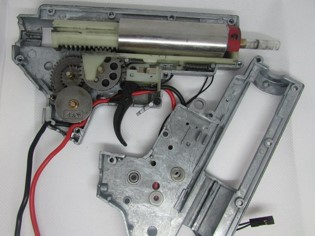
\includegraphics[width=0.6\linewidth]{gearboxbele}
	\caption{A gearbox belseje\cite{airsoft}}
	\label{fig:gearboxbele}
\end{figure}

A fegyver gearbox-ot körülvevő alkatrészeiről le tudtam venni méreteket, ez alapján alakítottam ki később a 3D nyomtatott alkatrészeket. Így végeredményben egy magába zárt alkatrészem lett, amin habár mechanikus nem lehet állítani a tüzelés módját, de csupán két vezetékkel csatlakozik az elektronikához. \\

A gearbox áramfogyasztását illetően találtam méréseket az internet, ahol kifejezetten az én modellemet tesztelték. Az Itteni mérések alapján arra következtettem, hogy 15 A-re méretezni az áramkört megfelelő lehet. \cite{airsoftteszt}

\subsubsection*{Motorok}

A projekthez kettő \textbf{NEMA-17} léptetőmotort használok\cite{nema17}. Ezek a léptetőmotorok egy széles körben alkalmazott típusa, amelyet főként precíziós mozgatási feladatokhoz használnak, például CNC gépekben, 3D nyomtatókban, robotikai alkalmazásokban és automatizálási rendszerekben. A NEMA-17 esetében a szám a motor elülső oldalának névleges méretét jelenti, amely 1.7 hüvelyk, azaz körülbelül 42,3 mm. \\

 A léptetőmotorok a mozgásukat apró, egyenlő lépésekre osztják, így lehetővé téve a precíz pozícionálást és sebességszabályozást. A NEMA-17 léptetőmotor tipikusan kétfázisú bipoláris motor, amely négy vezetékes tekercseléssel rendelkezik. Minden lépés során a motor egy adott szöggel fordul el, ami az adott motor típusától és felépítésétől függően tipikusan 1.8 fok, így teljes fordulat esetén 200 lépésre van szükség.\\

Az én esetemben használt léptetőmotorok lépésszöge 1.8 fok, bár ezt a motorvezérlőn lehet tovább osztani. A tartónyomatéka 0.4 Nm. Ezek a paraméterek 10-es áttételű fogaskerék-kapcsolattal megfelelőnek kell lenniük egy ilyen kis teljesítményű alkalmazásnál.

\pagebreak

\section{3D tervezés, modellezés}
A 3D tervezést Top-Down módszerrel végeztem, ez azt jelenti, hogy először az összeállítás szintjéről kezdem a tervezést, és egy úgynevezett skeleton modellbe veszem fel az egyes alkatrészek méreteit. Ezáltal tudom garantálni az egymáshoz való illeszkedést, valamint a változtatások könnyű implementálását.\\

\subsection{Skeleton modell}
A modellezést a skeleton modellek megalkotásával kezdtem. A fő összeállításon belül két skeleton modellt hoztam létre, mivel maga a modell két alösszeállítása jól elkülöníthető egymástól.

\begin{figure}[h!]
	\centering
	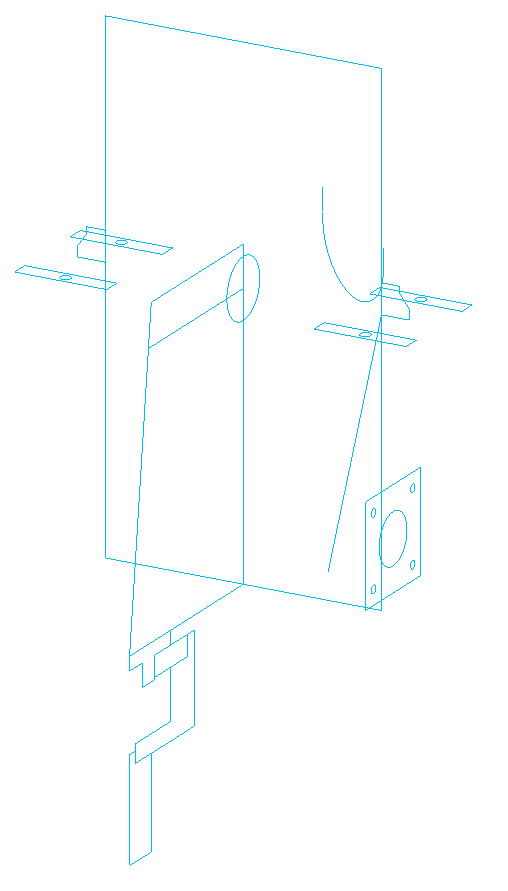
\includegraphics[width=0.5\linewidth]{mech_skeleton1}
	\caption{DT-9999 skeleton modell}
	\label{fig:mech_skeleton1}
\end{figure}

Az egyik (\ref{fig:mech_skeleton1}.ábra) alkatrészei rendszerint a függőleges tengely körül szimmetrikusak, a másiké (\ref{fig:mech_skeleton2}.ábra) pedig a fegyver csöve körül.

\begin{figure}[h!]
	\centering
	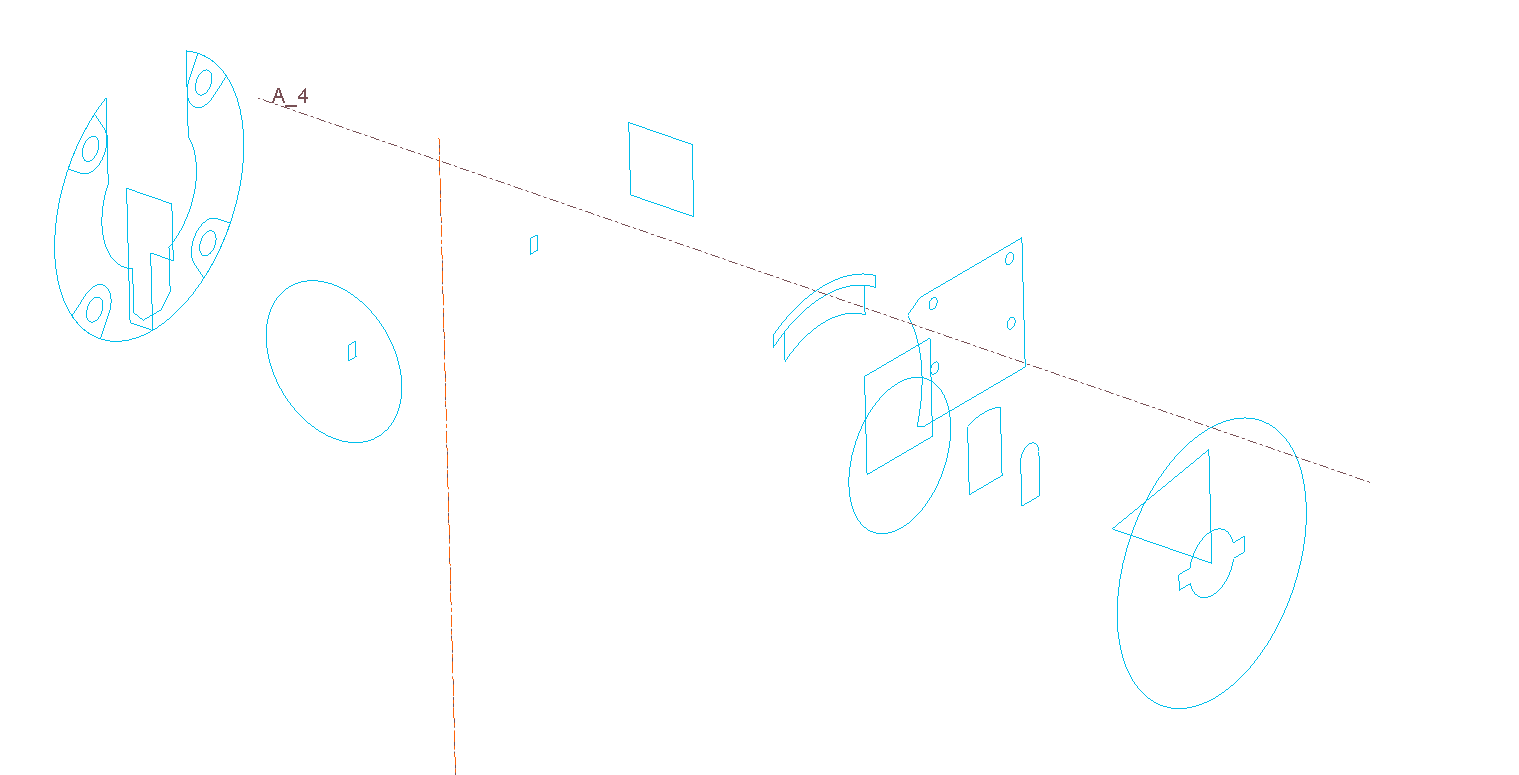
\includegraphics[width=1\linewidth]{mech_skeleton2}
	\caption{DT-4999 skeleton modell}
	\label{fig:mech_skeleton2}
\end{figure}

Az ábrákon láthatóak a vázlatok és tengelyek, amelyek alapján kialakítottam az egyes alkatrészeket. Sok méretet először csak hozzávetőlegesen vettem fel, pl. a torony magasságát. A Top-Down módszer előnye, hogy később ezeket könnyedén módosíthatom, és az alkatrészek frissítés után ugyanúgy fognak egymáshoz illeszkedni.


\subsection{Torony}

Elsőként a \textbf{gearbox tartó elemet} kezdtem el tervezni, mert maga a gearbox volt a tervezés elején az egyetlen elem, amiből tudtam következtetni a szükséges méretekre. Erről kép a \ref{fig:mech_dt4000}. ábrán látható. 

\begin{figure}[h!]
	\centering
	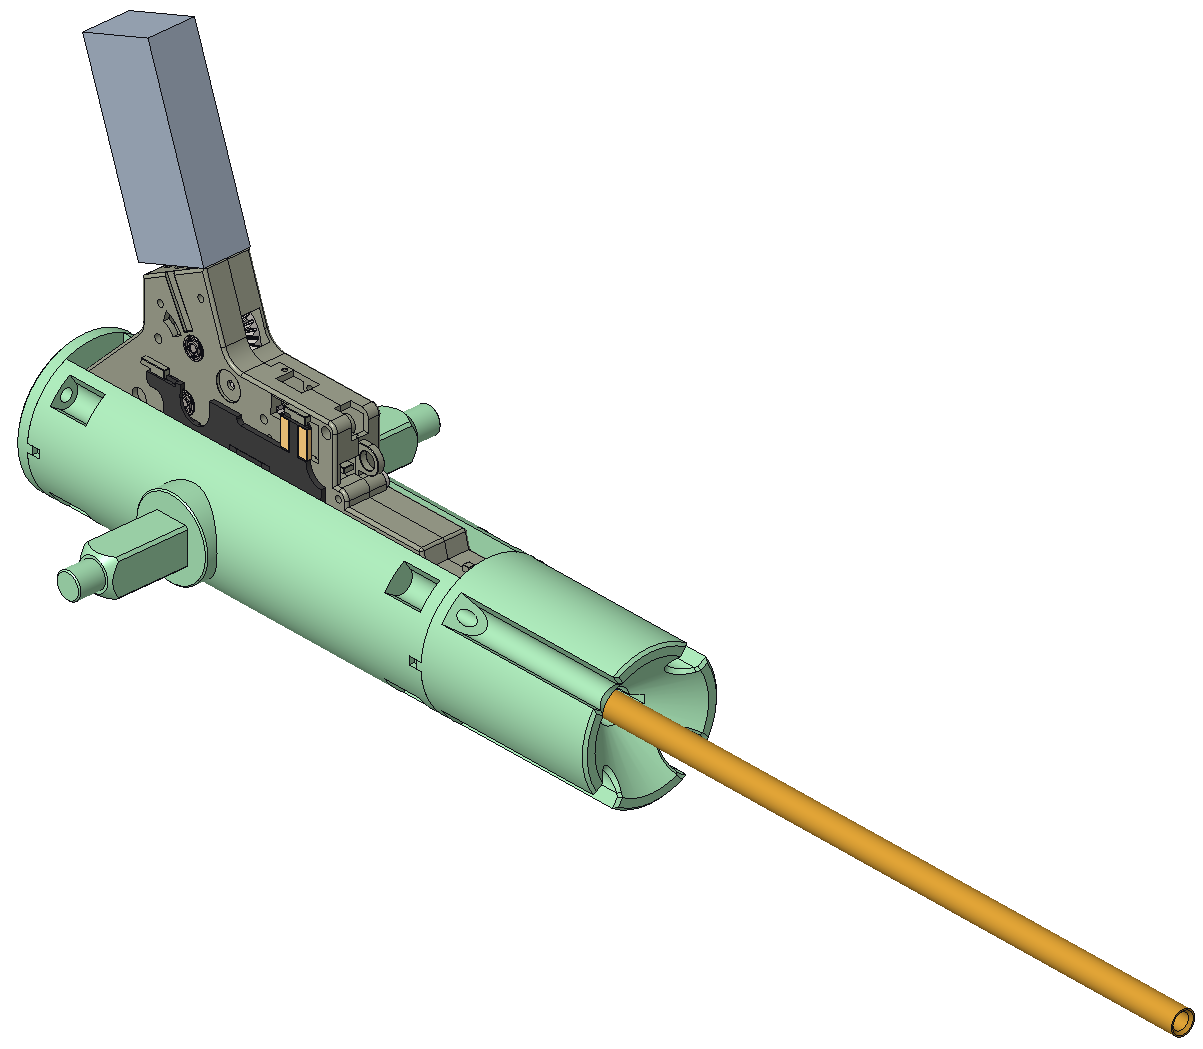
\includegraphics[width=0.8\linewidth]{mech_dt4000}
	\caption{Gearbox tartó ház}
	\label{fig:mech_dt4000}
\end{figure}

A gearbox ház 3 alkatrészből áll, egy központi elemből, valamint két fedélből a végein. A kialakítást a teljes airsoft fegyver alapján terveztem, hogy ugyanúgy álljon a gearbox mint az eredeti felhasználása során. A kritikusabb rész ebben az elemben a hop-up kamra körüli kialakítás volt, itt elég komplex volt a geometria, de a 3D nyomtatás lehetővé tette a megvalósítást. Ezt a \ref{fig:mech_dt4200}. ábrán lehet látni.


\begin{figure}[h!]
	\centering
	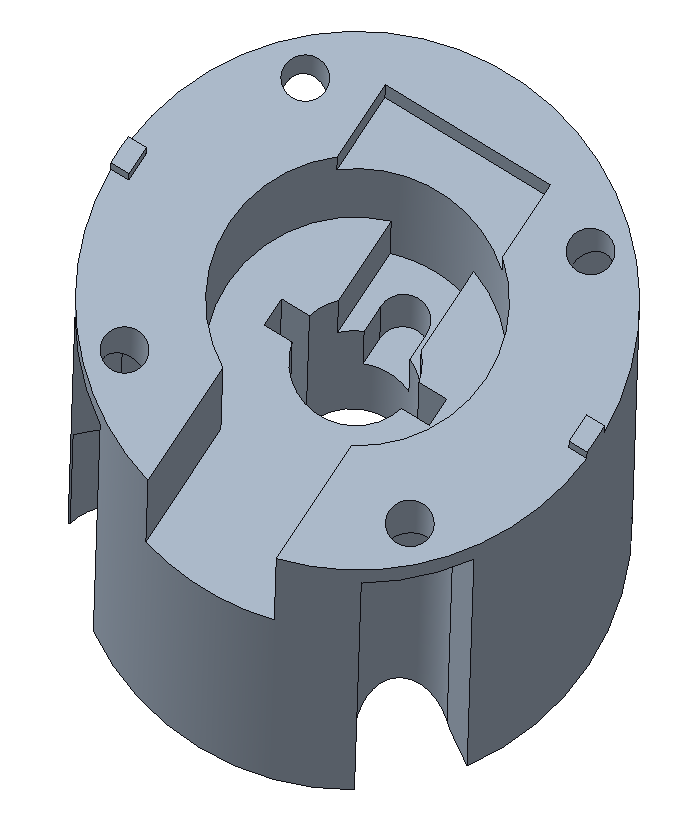
\includegraphics[width=0.4\linewidth]{mech_dt4200}
	\caption{Hop-Up kamra körüli elem}
	\label{fig:mech_dt4200}
\end{figure}


A következő alösszeállítás a \textbf{tár} volt, amely a gearbox ház bal oldali tengelyére csatlakozik. Ennek kialakítása a \ref{fig:mech_tar}. ábrán látható. A 6 mm-es golyók a zöld kupak nyílásán keresztül tölthetőek a lila tárba. Alul és felül 1-1 gumigyűrű feszíti előre a zöld dugattyút, ami a tár kúpos végén keresztül nyomja ki a golyókat. Így mechanikailag, plusz elektronika nélkül biztosítható a fegyver lövedékkel való ellátása, és szemmel is látható a tár töltöttségi szintje.

\begin{figure}[h!]
	\centering
	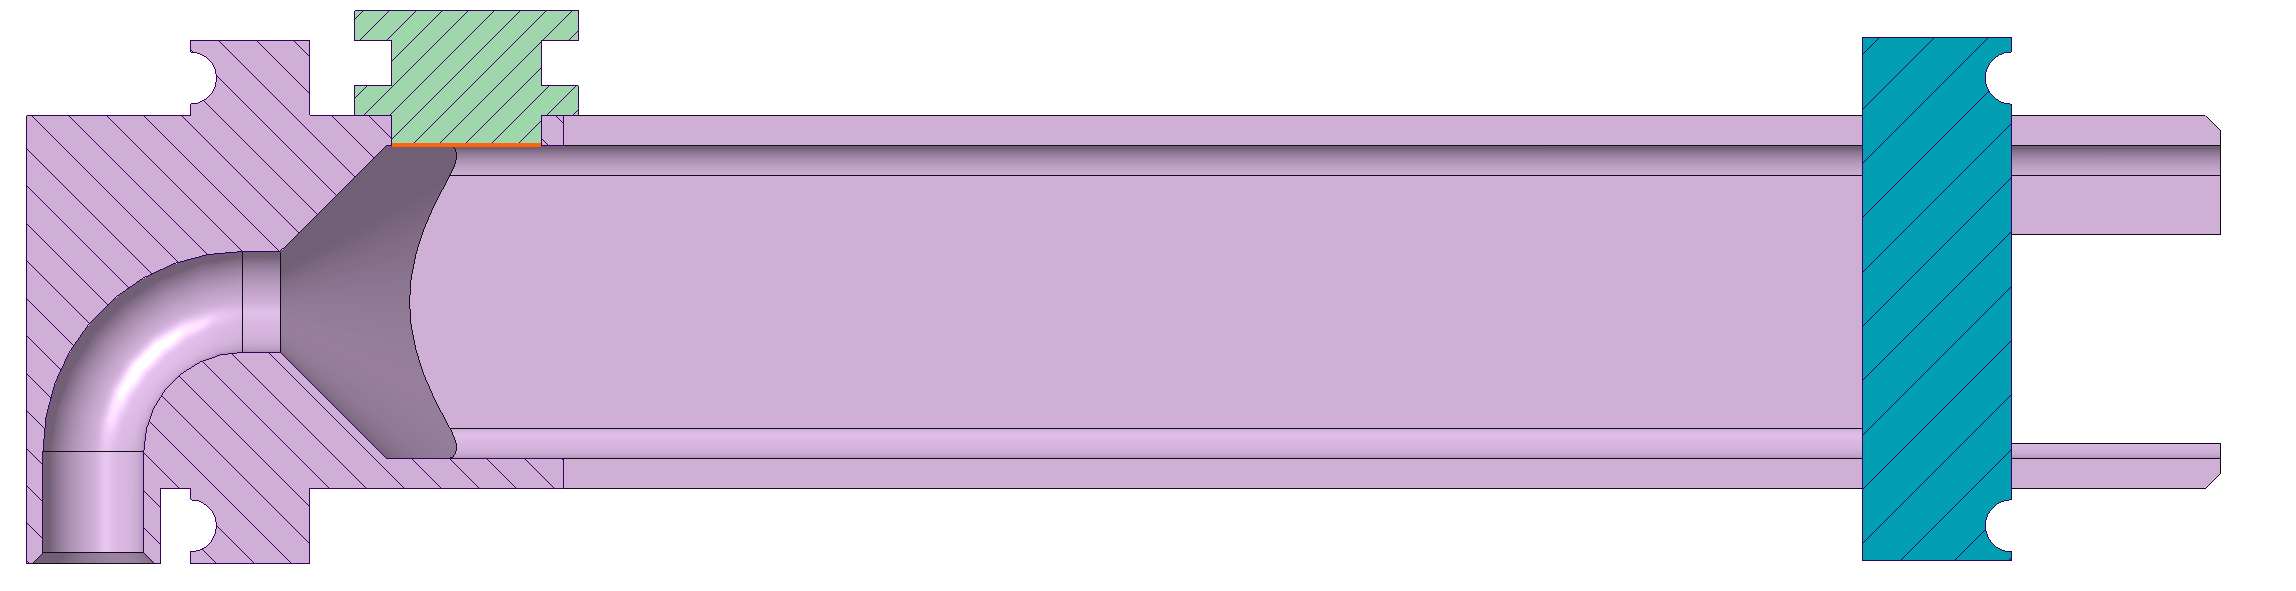
\includegraphics[width=1\linewidth]{mech_tar}
	\caption{Tár}
	\label{fig:mech_tar}
\end{figure}

Ez a kialakítás végül nem volt sikeres, ugyanis a golyók nagyon könnyedén elakadtak, gyakorlatilag egyszer sem sikerült lőni vele. Újragondolás után egy hasonló megoldást használtam, ám a golyók egyesével sorakoznak a tárban, ez láthat a \ref{fig:mech_tar2}. ábrán.



\begin{figure}[h!]
	\centering
	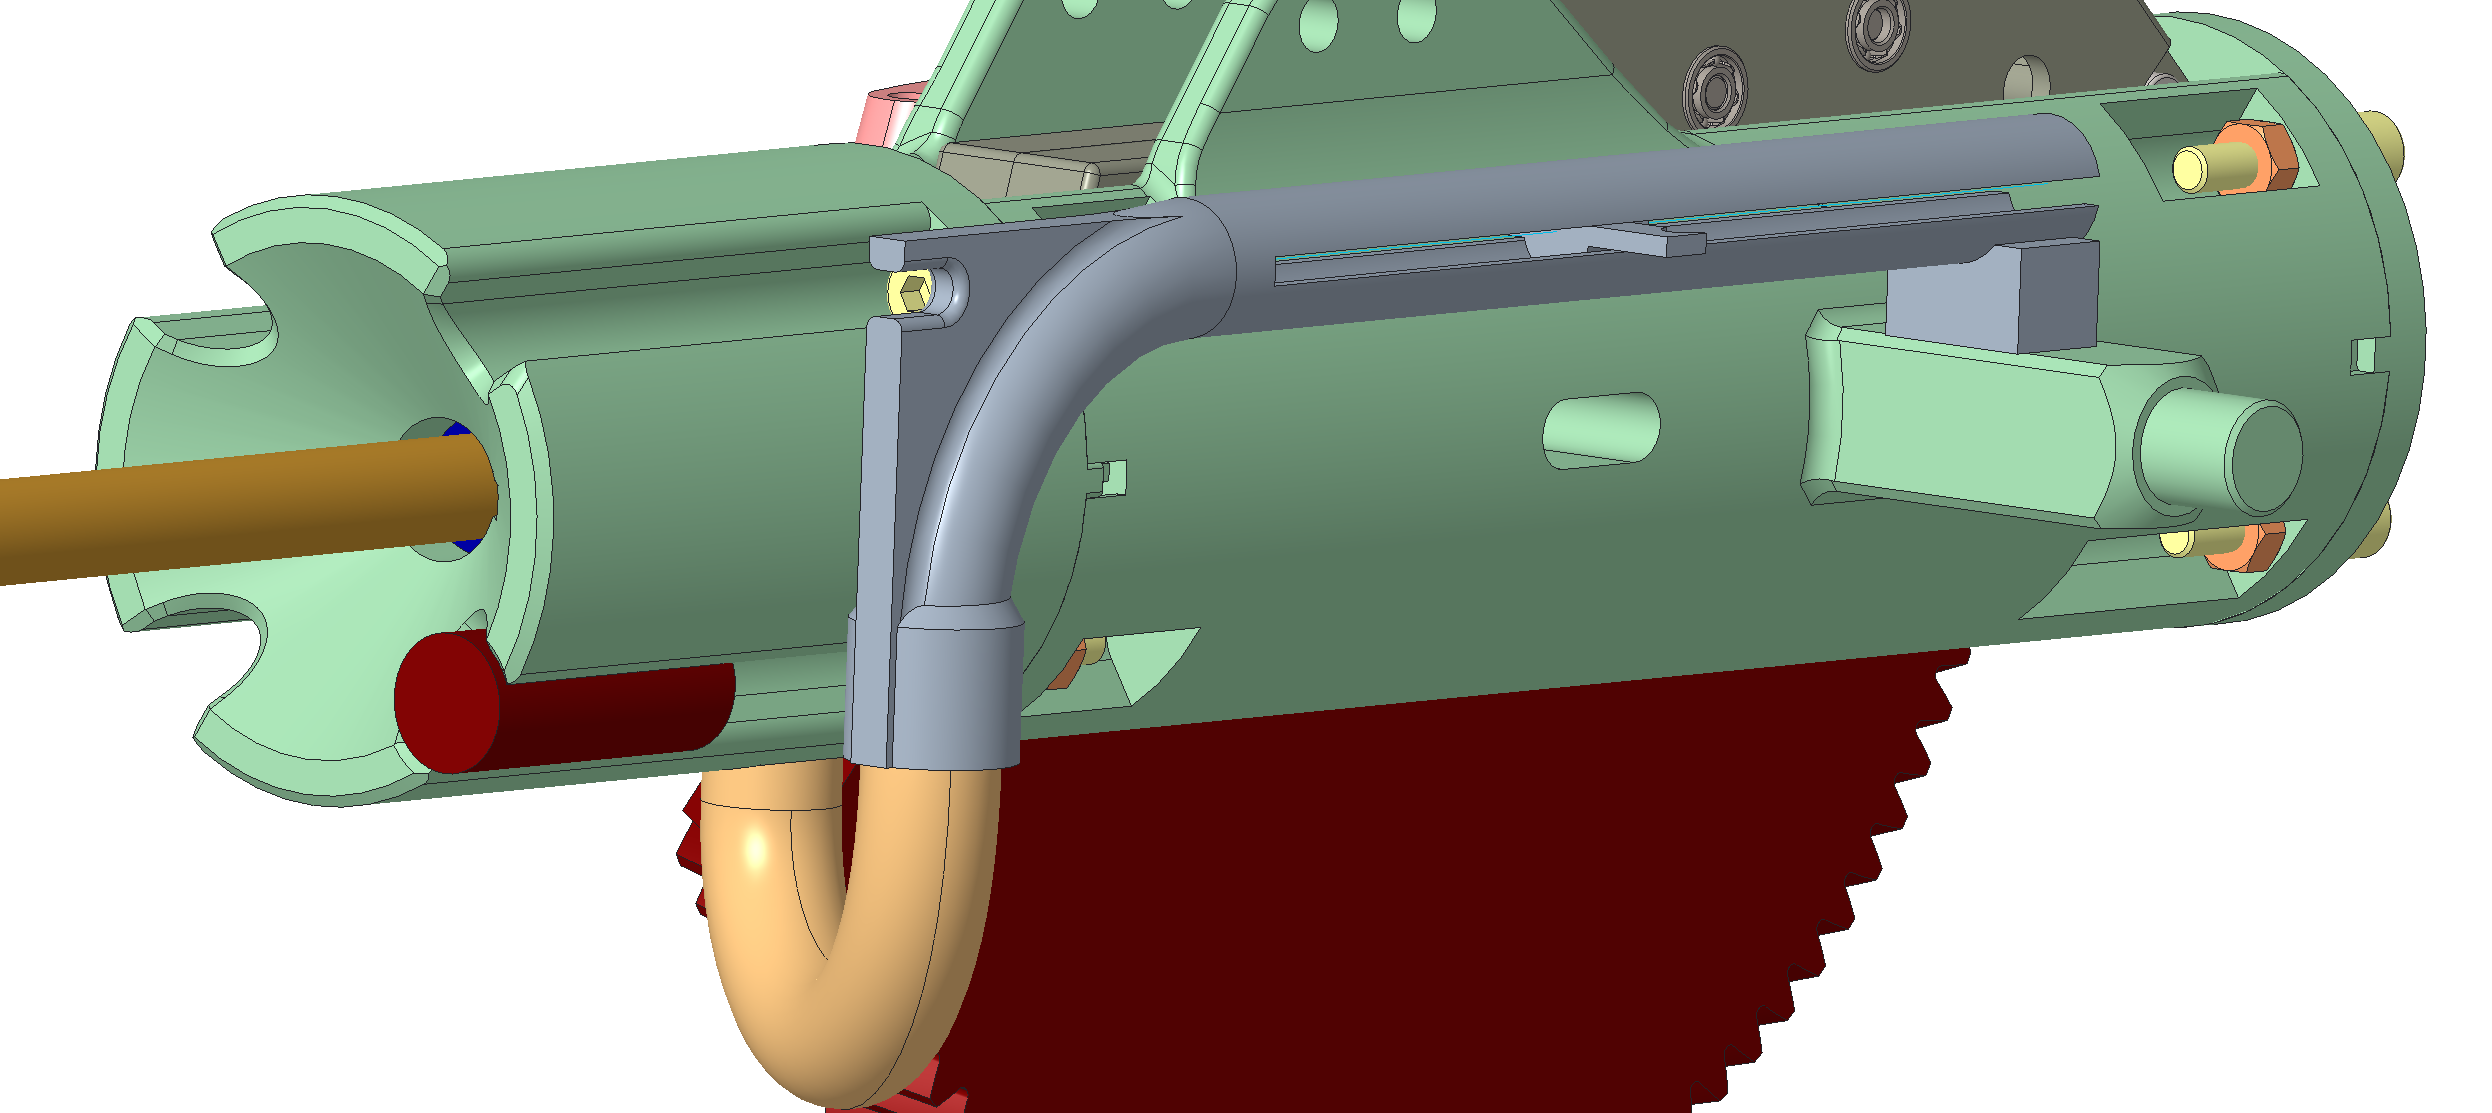
\includegraphics[width=1\linewidth]{mech_tar2}
	\caption{Új tár}
	\label{fig:mech_tar2}
\end{figure}
Végül a toronyra kerültek az elektronikai alkatrészek is, ezek a \ref{fig:mech_dt4000kamera}. ábrán láthatóak. A lila elem a lézer modul, a piros pedig a kamera konzol. Mind a kettő ragasztással kerül rögzítésre. Fontosnak tartottam, hogy ezek az elemek közvetlenül ahhoz az elemhez legyenek rögzítve, ami a fegyver csövét is pozicionálja, azonban a kamera esetén a 3D nyomtathatóság miatt egy konzolt szükségesnek éreztem.

\begin{figure}[h!]
	\centering
	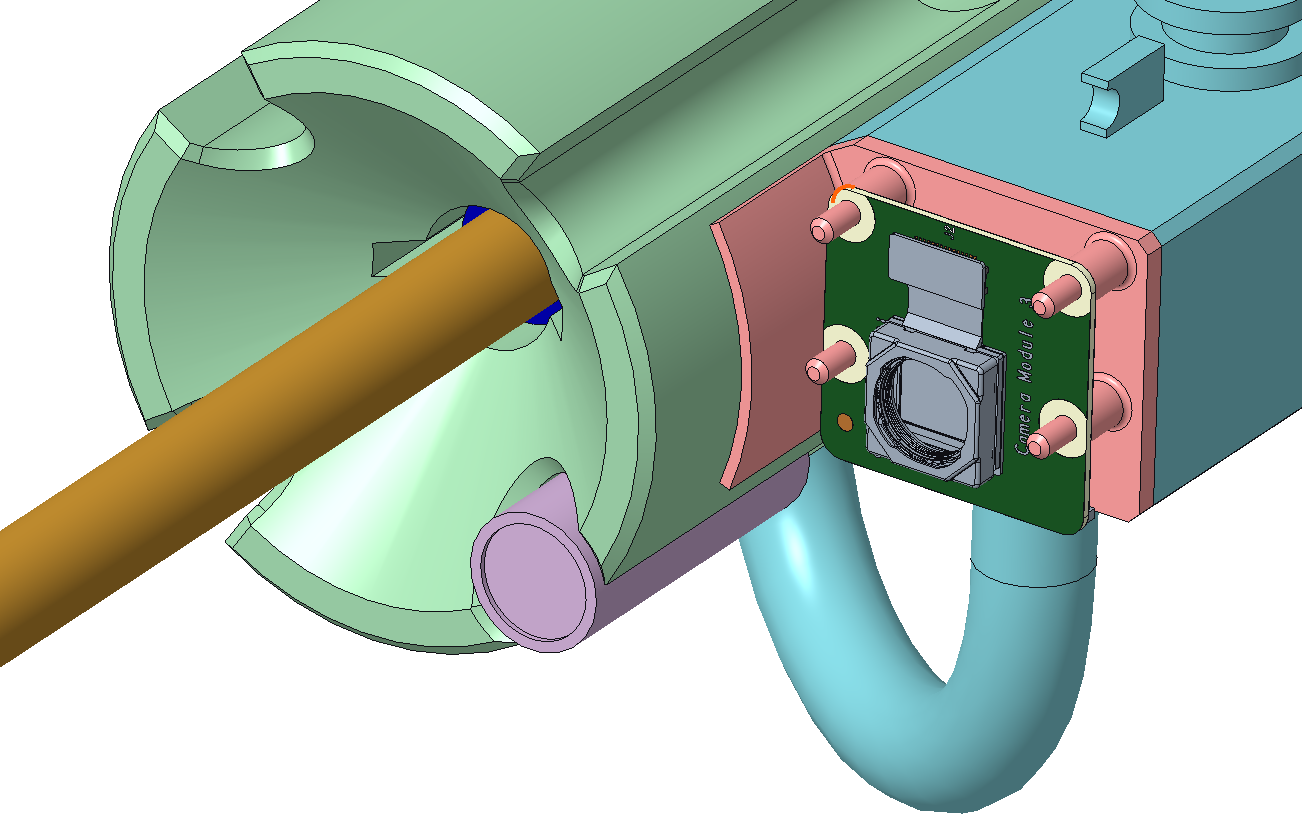
\includegraphics[width=1\linewidth]{mech_dt4000kamera}
	\caption{Kamera és lézer modul beépítés}
	\label{fig:mech_dt4000kamera}
\end{figure}

\subsection{Keret}
Az úgynevezett \textbf{keret} volt a konstrukció legösszetettebb eleme, és egyben a legnagyobb térfogatú is. Fő funkciója a torony stabil tartása a csapágyakkal együtt. Ezentúl erre az elemre van rögzítve a vezérlőelektronika nagy része, a végálláskapcsolók és a vízszintes tengelyhez tartozó motor is. Ez az elem az alatta lévő alkatrészhez ragasztással lett rögzítve, hogy a szerelést egyszerűsítsem. A csapágyak támasztása X elrendezésű, és az osztott "csapágyház" miatt könnyen szerelhetőek. A csapágy elrendezése a \ref{fig:mech_felsotengely}. ábrán látható.

\begin{figure}[h!]
	\centering
	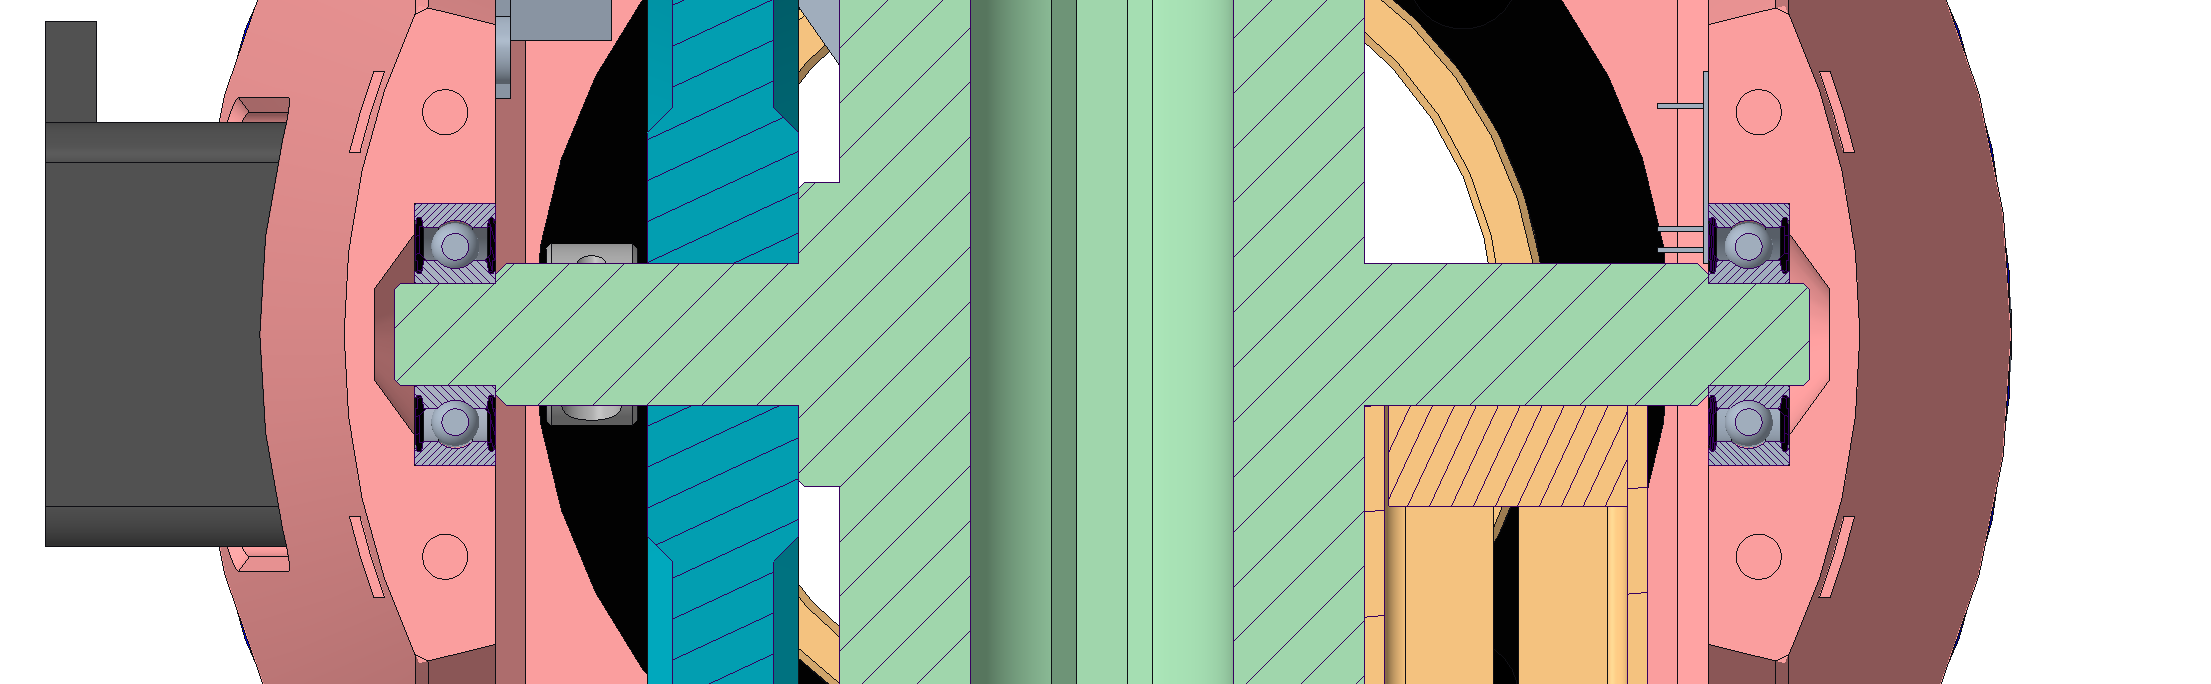
\includegraphics[width=1\linewidth]{mech_felsotengely}
	\caption{Vízszintes tengely csapágyainak elrendezése}
	\label{fig:mech_felsotengely}
\end{figure}


Kétséges rész volt a \textbf{motor} rögzítése, ugyanis nagy szükség van a pontos illeszkedésre. A nyomtatás irányára azonban a motor központosítására szánt furat pont merőleges, de szerencsére a nyomtató így is elég nagy pontosságot tudott elérni.

\begin{figure}[h!]
	\centering
	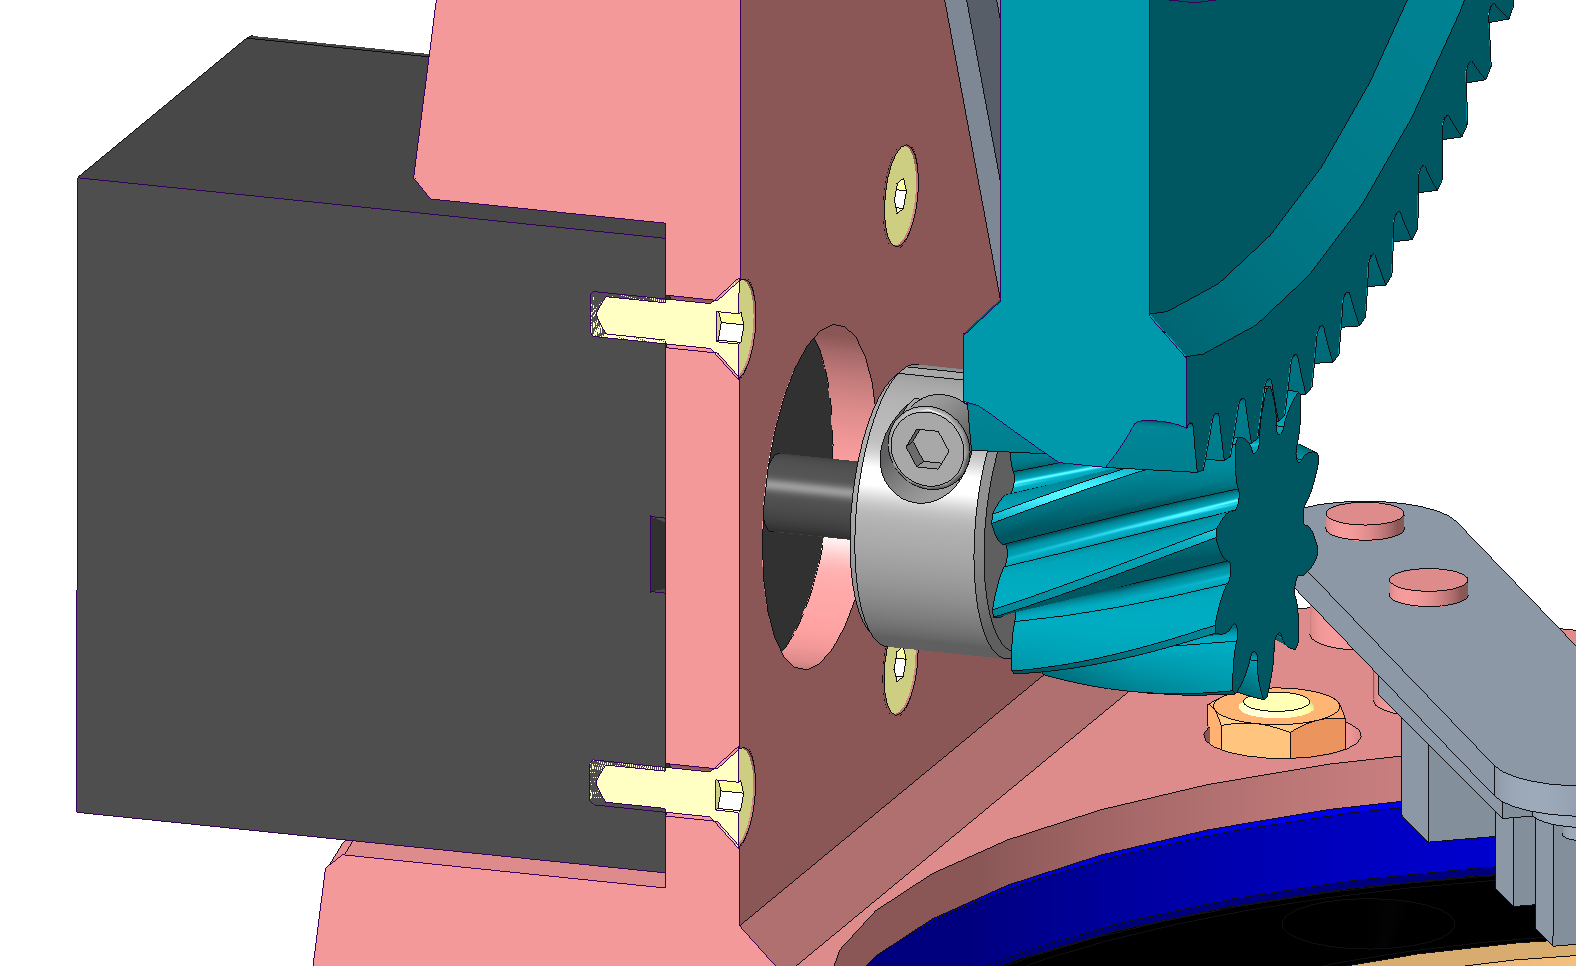
\includegraphics[width=1 \linewidth]{mech_motorbeepites}
	\caption{Vízszintes tengely motor beépítése}
	\label{fig:mech_motorbeepites}
\end{figure}

A kereten kaptak helyet a végálláskapcsolók is, amivel a rendszer indításkor kalibrálható. A egyik a vízszintes tengely nagy fogaskerekét, a másik pedig a függőleges tengely központi eleméhez viszonyít.


\begin{figure}
	\centering
	\begin{minipage}{.5\textwidth}
		\centering
		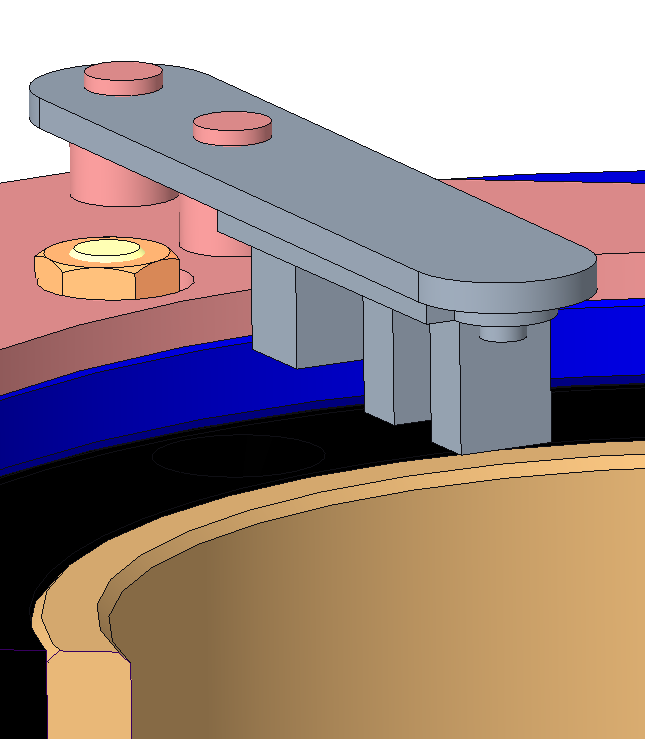
\includegraphics[width=.7\linewidth]{mech_vegallas1}
		\caption{Pan végálláskapcsoló}
		\label{fig:mech_vegallas1}
	\end{minipage}%
	\begin{minipage}{.5\textwidth}
		\centering
		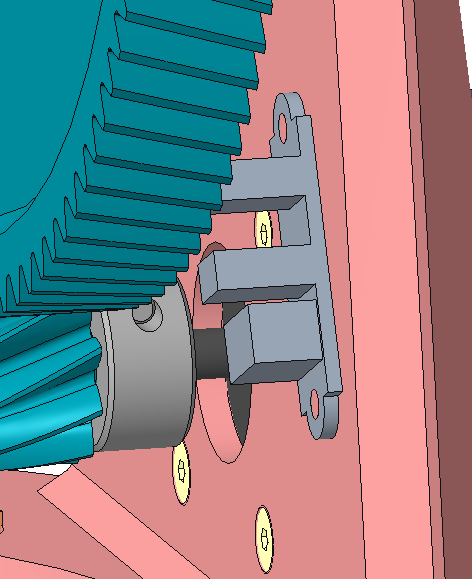
\includegraphics[width=.7\linewidth]{mech_vegallas2}
		\caption{Tilt végálláskapcsoló}
		\label{fig:mech_vegallas2}
	\end{minipage}
\end{figure}

\subsection{Függőleges tengely elemei}

Utolsó lépésként megterveztem a függőleges tengely mozgatásáért felelős elemeket. ezek kialakítása a \ref{fig:mech_alsoreszek}. ábrán látható. A narancssárga alakrész a központi elem, amelynek feladata a csapágy támasztása és a motor rögzítése. A motor vezetékei, valamint az elektronikából kilógó többi kábel ennek a közepén fut keresztül. A csapágy egyik fele ehhez az elemhez van rögzítve, a másik pedig  az ábrán kékkel ábrázolt alkatrészhez. Erre a kék elemere került rögzítésre a belsőfogazású fogaskerék is. \\ 

A sárga alkatrész a talapzat része. Ez a legnagyobb kiterjedésű elem az egész modellben. Hogy elkerüljem a támaszanyag használatát, a csavarok fejeinek felfekvő felületeti egy külön alkatrész ragasztásával oldottam meg. Ez a talp 45 fokos belső felületére illeszkedik, és ragasztással kerül rögzítésre. A 4 oldalán kialakításra kerültek csatlakozó felületek, ahol különböző lábak helyezhetők az eszközre.

\begin{figure}[h!]
	\centering
	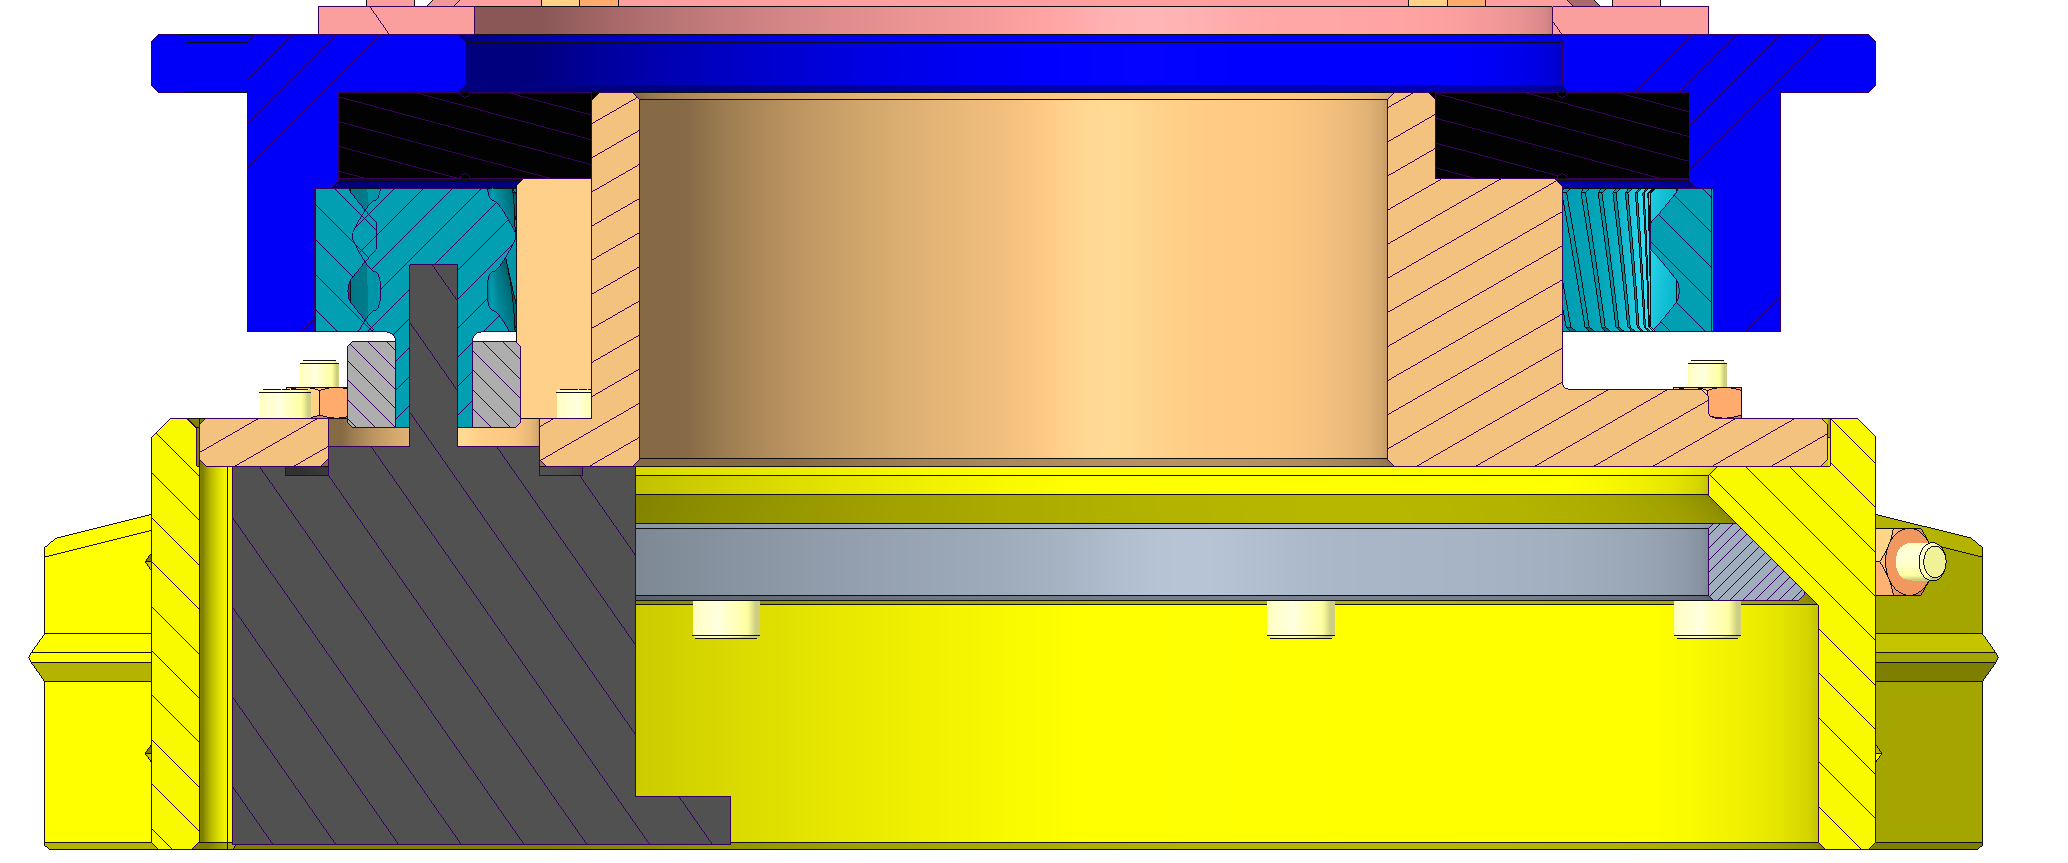
\includegraphics[width=1\linewidth]{mech_alsoreszek}
	\caption{Függőleges tengely elrendezése}
	\label{fig:mech_alsoreszek}
\end{figure}

\subsection{Fogaskerekek}
A prototípusban két fogaskerék kapcsolat kapott helyet. A függőleges tengely nagy fogaskereke belső fogazású, ezáltal el tudtam rejteni a motort a váz belsejében és kompaktabb lett a kialakítás, valamint valamivel stabilabb is. A kapcsolat áttétele 10, és ferde fogazású, ezáltal a futás csendesebb és egyenletesebb lett. A kapcsolat illusztrációja a \ref{fig:mech_fogpar1}. ábrán látható.

\begin{figure}[h!]
	\centering
	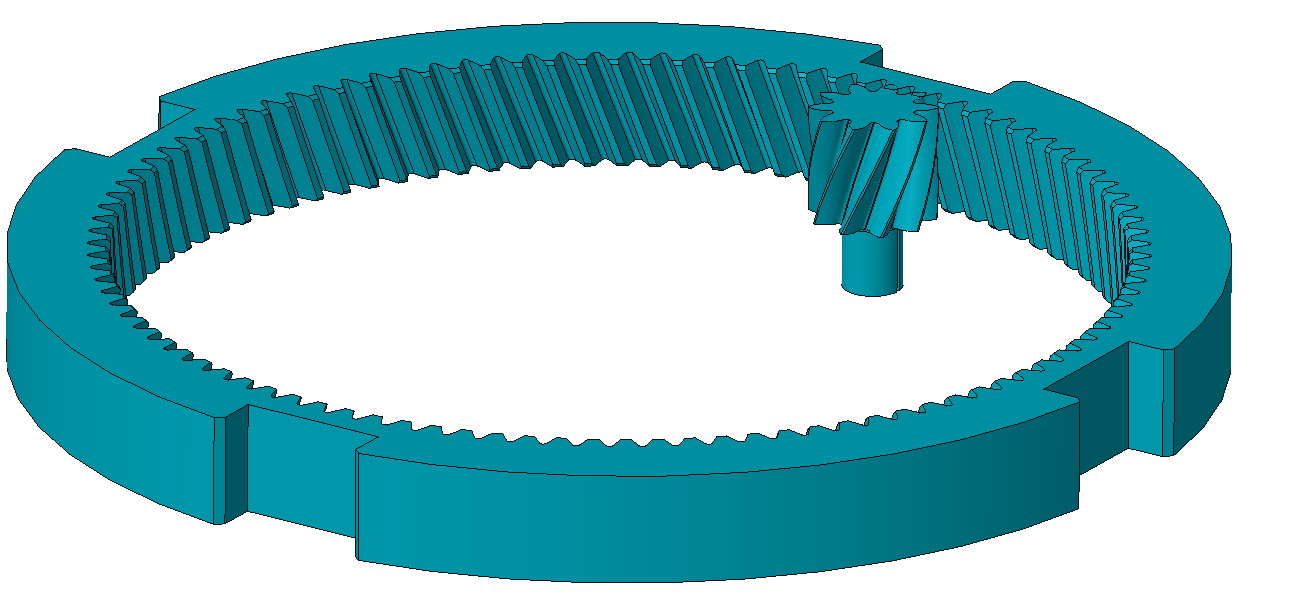
\includegraphics[width=1\linewidth]{mech_fogpar1}
	\caption{Függőleges tengely fogaskerekek}
	\label{fig:mech_fogpar1}
\end{figure}

A vízszintes tengely nagy fogaskereke a gearbox ház tengelyére lett erősítve, és csak részlegesen lett kinyomtatva. Ennek egyszerű oka, hogy más geometria is blokkolja a mozgást ezekben a tartományokban, illetve a Pan-Tilt kinematika mozgása redundáns lenne, ha teljesen körbe tudna forogni. A kapcsolat a \ref{fig:mech_fogpar1}. ábrán látható.

\begin{figure}[h!]
	\centering
	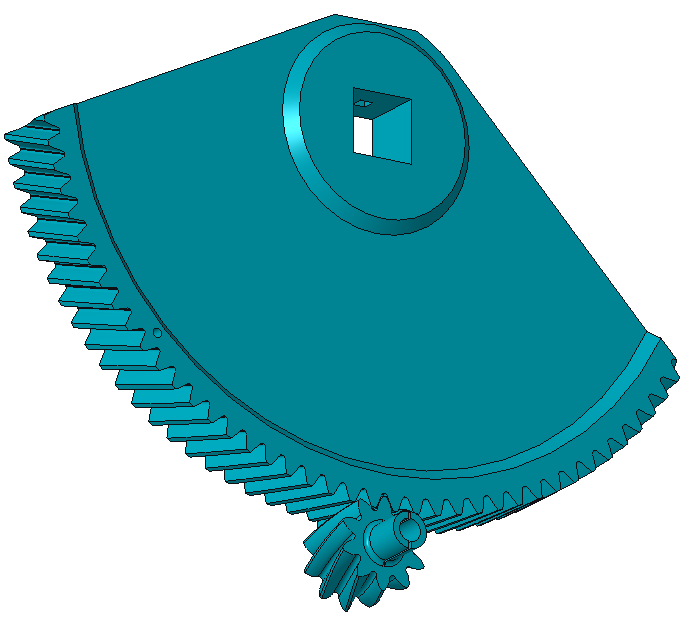
\includegraphics[width=0.5\linewidth]{mech_fogpar2}
	\caption{Vízszintes tengely fogaskerekek}
	\label{fig:mech_fogpar2}
\end{figure}

Mind a két fogaskerékpár kisebb közvetlenül a motor tengelyére lett rögzítve, egy acél rögzítőgyűrűvel. Ennek kialakítása a \ref{fig:mech_alsoreszek}. ábra bal oldalán látható.

\pagebreak

\section{Gyártás és összeszerelés}
\subsection{Gyártás}



Minden egyedi alkatrészt, amit a projekthez kellett gyártanom, 3D nyomtatással készítettem el. Ehhez egy \textbf{Bambu Lab A1} \cite{bambu} típusú hobbinyomtatót használtam, amely a \ref{fig:mech_bambu}. ábrán látható. Mint a legtöbb ilyen árkategóriában lévő gép, ez is \textsl{FDM} technológiát használ. Az \textsl{FDM} lényege, hogy a nyomtató egy előre megadott terv alapján vékony műanyagszálat (filamentet) olvaszt meg egy forró extruderfejben (hotend), amelyet pontosan irányítanak a nyomtató XYZ tengelyei mentén. A műanyag szál olvasztott állapotban kerül a nyomtatóágyra, ahol gyorsan megszilárdul, így rétegenként építi fel az adott objektumot.\\

\begin{figure}[h!]
	\centering
	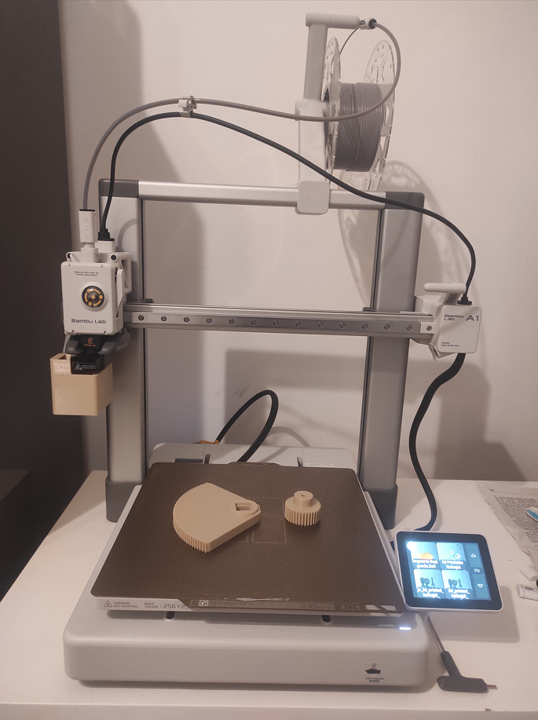
\includegraphics[width=.7\linewidth]{mech_bambu} 
	\caption{Bambu Lab A1}
	\label{fig:mech_bambu}
\end{figure}
\pagebreak

A használt nyomtató bizonyos tulajdonságai meghatározták a tervezett alkatrészek tulajdonságait:

\begin{itemize}
	\item \textbf{Nyomtatási térfogat:} 256 × 256 × 256 mm, amely elég nagy volt a legtöbb általam tervezett elem számára.
	\item \textbf{Nyomtatási pontosság:} Az nyomtató rétegvastagsága 0,1–0,4 mm között állítható. Főleg a nyomtatott fogaskerekeknél volt fontos a megfelelő pontosság, de kielégítő eredmény született.
	\item \textbf{Használható filamentek:} A nyomtató különféle anyagokkal kompatibilis, beleértve a PLA-t, ABS-t, PETG-t és TPU-t. Én a PLA mellett döntöttem, ugyanis nem szükséges a pl. ABS által nyújtott minőség, ellenben a költséghatékonyság igen.
\end{itemize}

A modelleket \textbf{PTC Creo} szoftverben készítettem. Ez egy magas szintű CAD tervező program, amely képes a modelleket exportálni STEP és STL fájlként is. Az STL fájlokat ezután a Bambu Studio slicer programba betöltve tudtam a nyomtató által követhető G-kódra konvertálni. Itt kellett megtervezni a támasztást (\ref{fig:mech_bambustudio1}. ábra), illetve megadnia a nyomtatási paramétereket, amelyek a függelék \ref{sec:slicerbeallitasok}. fejezetében láthatóak. Ezután már csak meg kellett várni, amíg a gép elkészíti az adott alkatrészt, ami a legnagyobb elem esetén kb. 10 óra volt, a teljes prototípus kb. 50 óra volt.

\begin{figure}[h!]
	\centering
	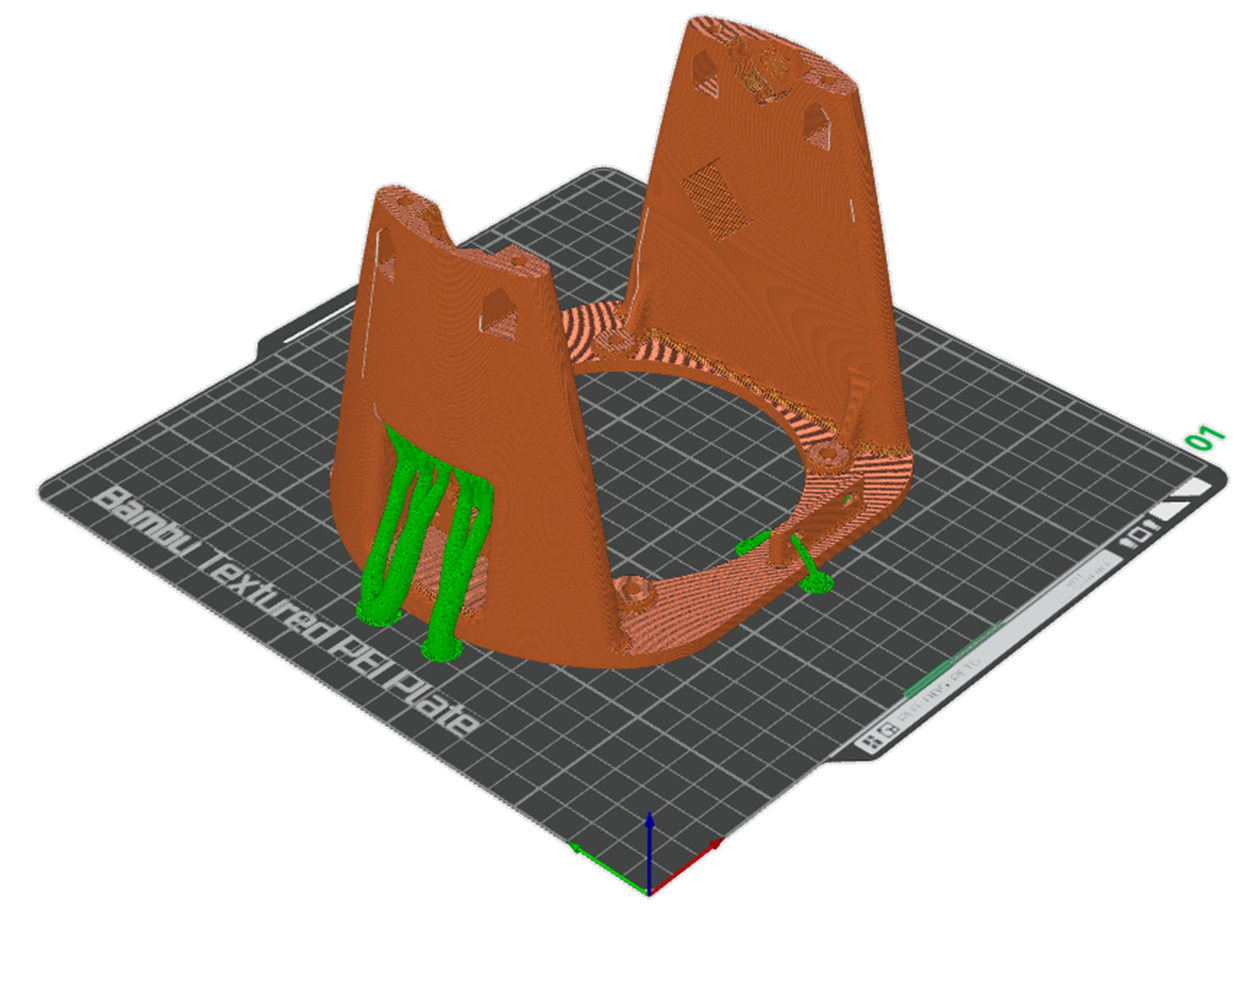
\includegraphics[width=.7\linewidth]{mech_bambustudio1} 
	\caption{Bambu Studio Slicer}
	\label{fig:mech_bambustudio1}
\end{figure}

\pagebreak
\subsection{Összeszerelés}

Ebben a fejezetben leírom az összeszerelés menetét. Először az elektronikát tartó konzollal kezdtem.

\begin{enumerate}
	\item Ráhúztam a motorok tengelyére a kisfogaskerekeket. 
	\item Rácsavaroztam a távtartókat a Raspberry Pi-ra, a Stepper Motor HAT-ra és a DCDC konverterre, majd mind a hármat rácsavaroztam a 3D nyomtatott konzolra. Félretettem az összeállítást.
	\item Összeraktam a torony elemeit, a gearboxot, a tartó elemét és a két végén lévő elemeket. Összecsavaroztam a tervezett furatokon, majd ezt az összeállítást is félretettem. 
	\item Összeállítottam a prototípus 4 lábát és az ezeket tartó hengert. A lábak talpára gumi elemeket ragasztottam, hogy minél stabilabban legyen a rendszer. Félretettem száradni.
	\item Ezután összecsavaroztam a nagy csapágyhoz csatlakozó alkatrészeket, illetve a DT-1000 elemhez rögzítettem az egyik motort. A DT-2000 elemhez ragasztottam a hozzá tartozó fogaskereket.
	\item A prototípus talpát összecsavaroztam az előző pontban lévő elemmel úgy, hogy a keretet is tartsák a csavarok.
	\item A kerethez rögzítettem a megfelelő motort, beragasztottam a relét és a végálláskapcsolókat is. Kábelkötözővel rögzítettem az elektronikai elemek konzolját a kerethez.
	\item A korábban összerakott gearbox összeállítás tengelyeire illesztettem az oda tartozó fogaskereket és a csapágyakat. Így ráhelyeztem a keretre, és a csapágyházak felső felét hozzácsavaroztam a keretre. 
	\item Összeillesztettem a kamera konzolt, és felragasztottam a helyére. Ugyanígy tettem a tárral is. Beillesztettem a lézer modult a helyére.
	\item Összekötöttem a kábeleket, csatlakozókat.
	\item Csatlakoztattam a tápokat és az ethernet-kábelt.
\end{enumerate}
Az elkészült eszközt a \ref{fig:sentry1}. ábrán lehet látni.
\pagebreak

\begin{figure}[h!]
	\centering
	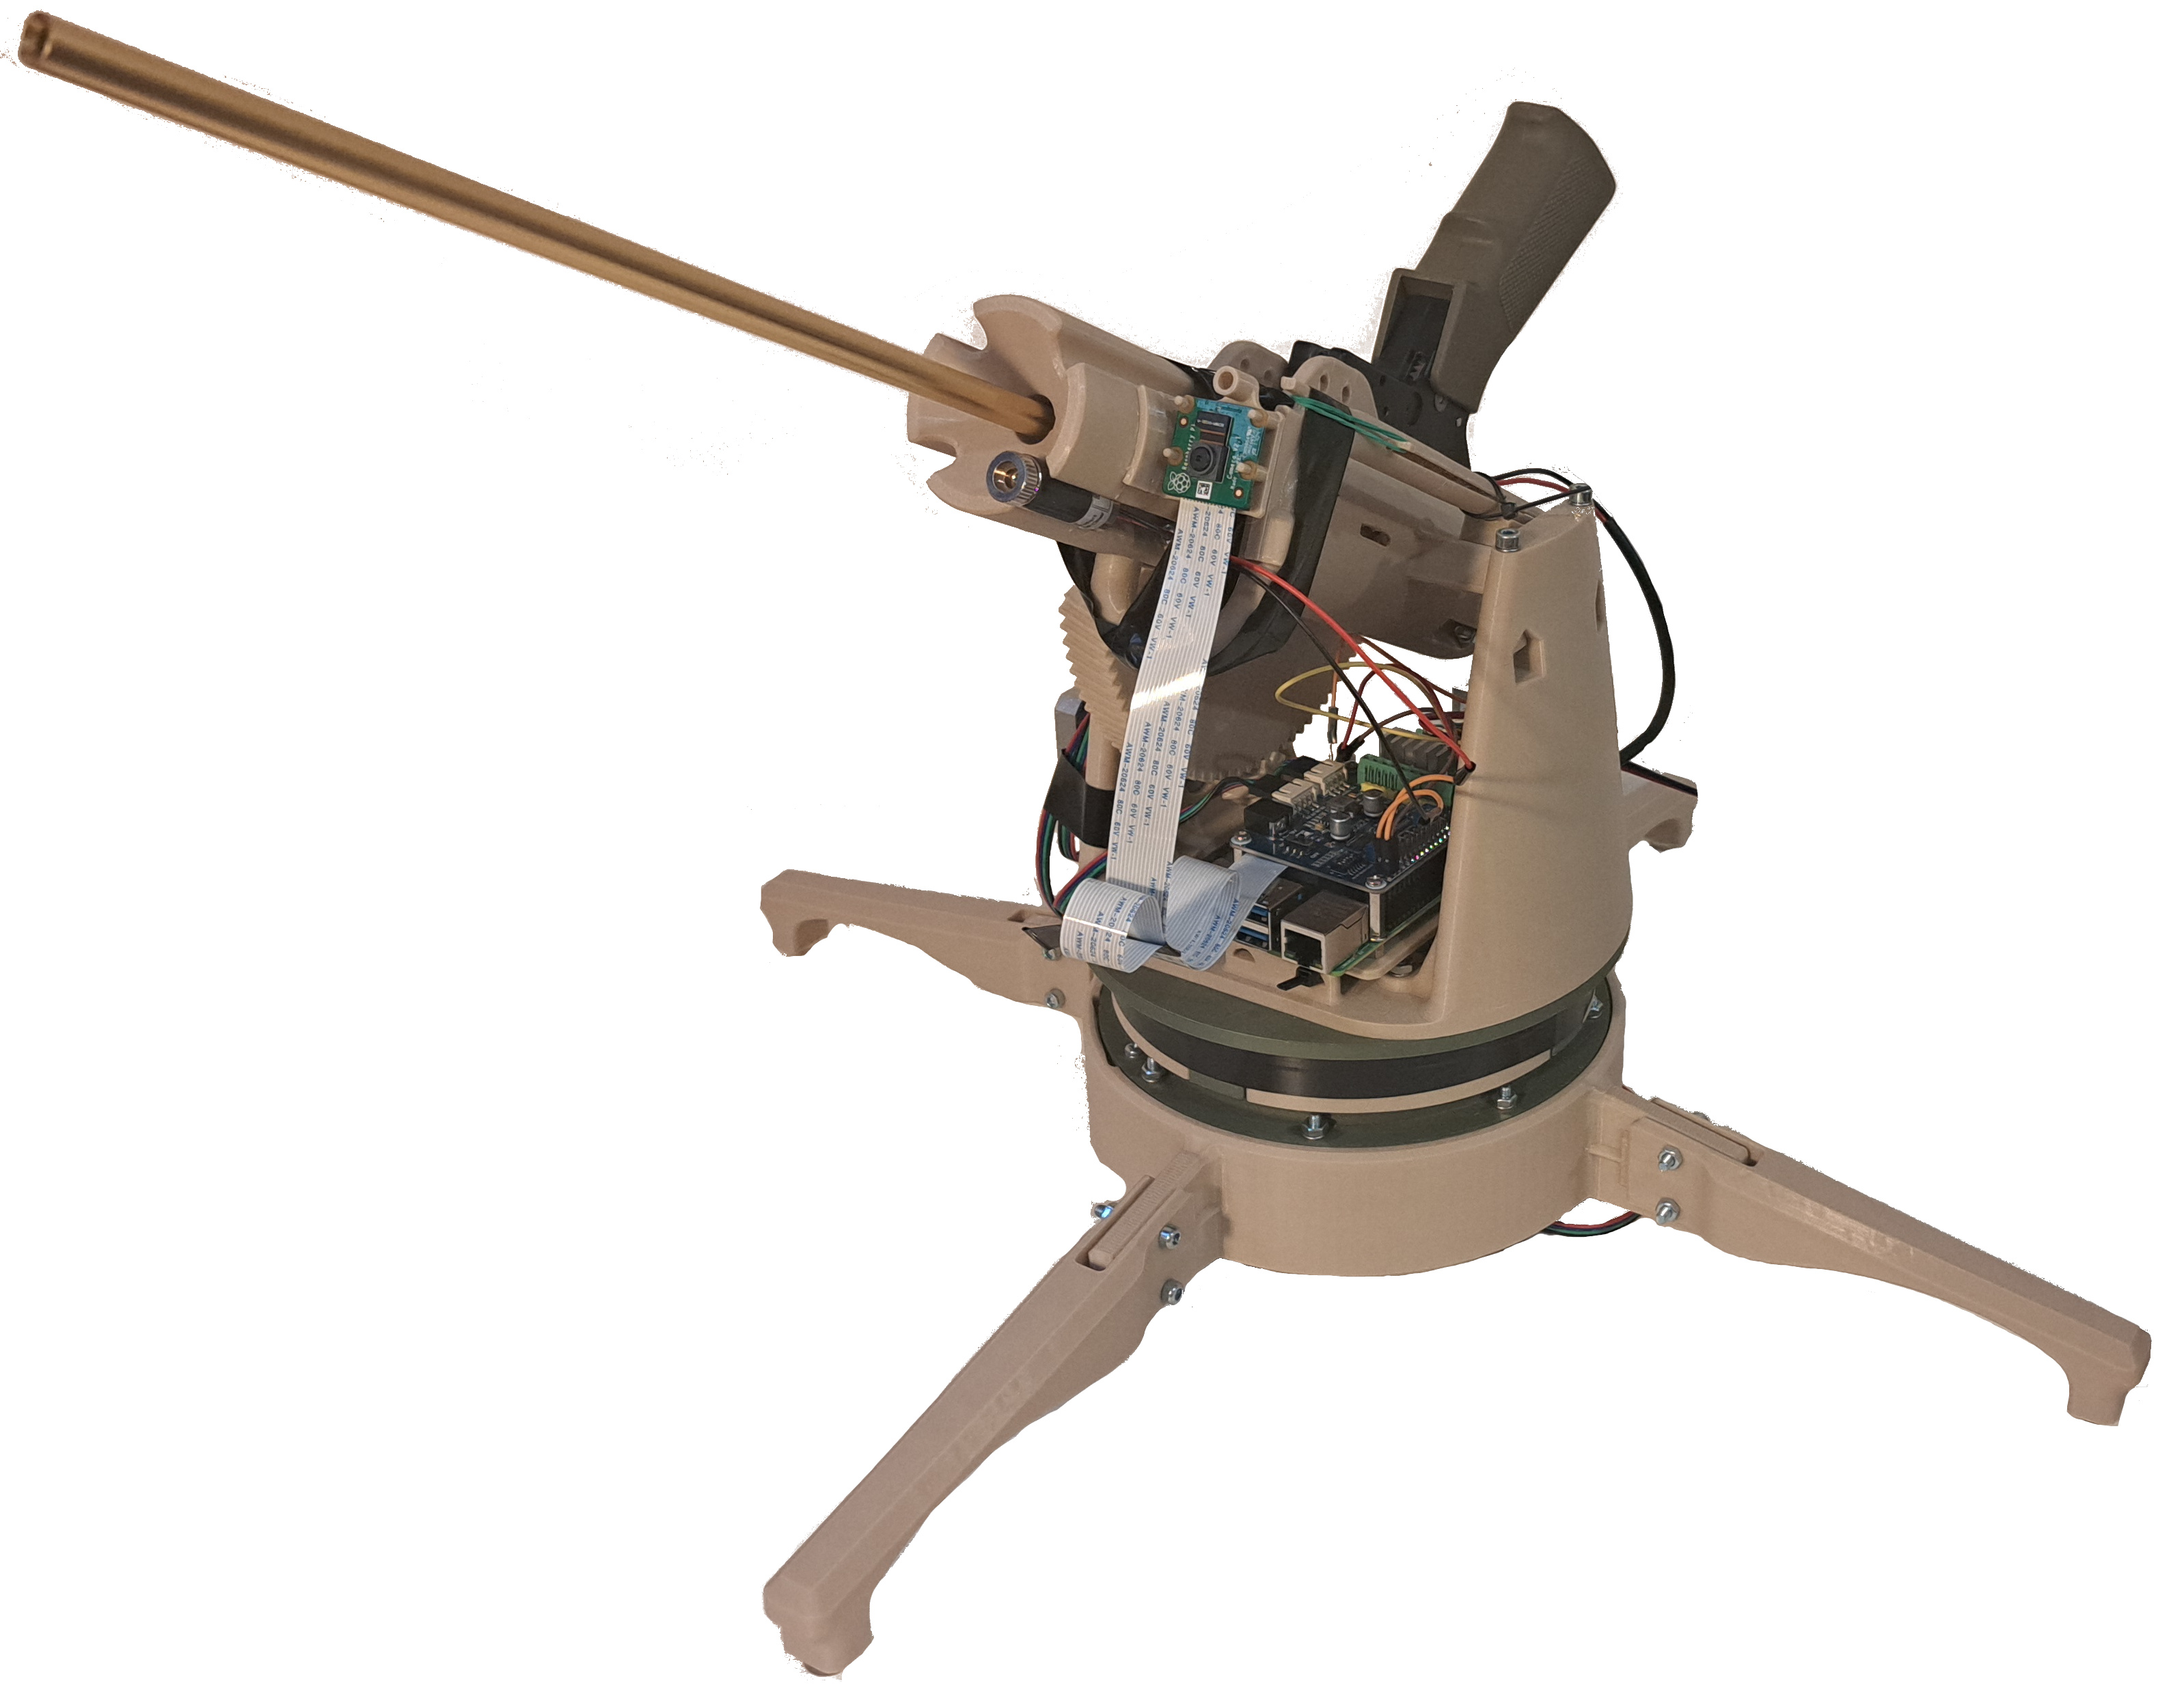
\includegraphics[width=1\linewidth]{sentry1}
	\caption{Összeállított prototípus}
	\label{fig:sentry1}
\end{figure}
\chapter{Hardvertervezés}

\section{Áramköri tervezés}
A prototípus áramkörét próbáltam minél egyszerűbben megvalósítani. Alapvetően két részből áll, a Raspberry PI központú vezérlőáramkörből, ami felelős a szenzorokért és a Raspberry PI-ért, illetve egy nagyobb teljesítményű áramkör egy külön tápról, ami a gearbox működtetéséért felelős.


\begin{figure}[h!]
	\centering
	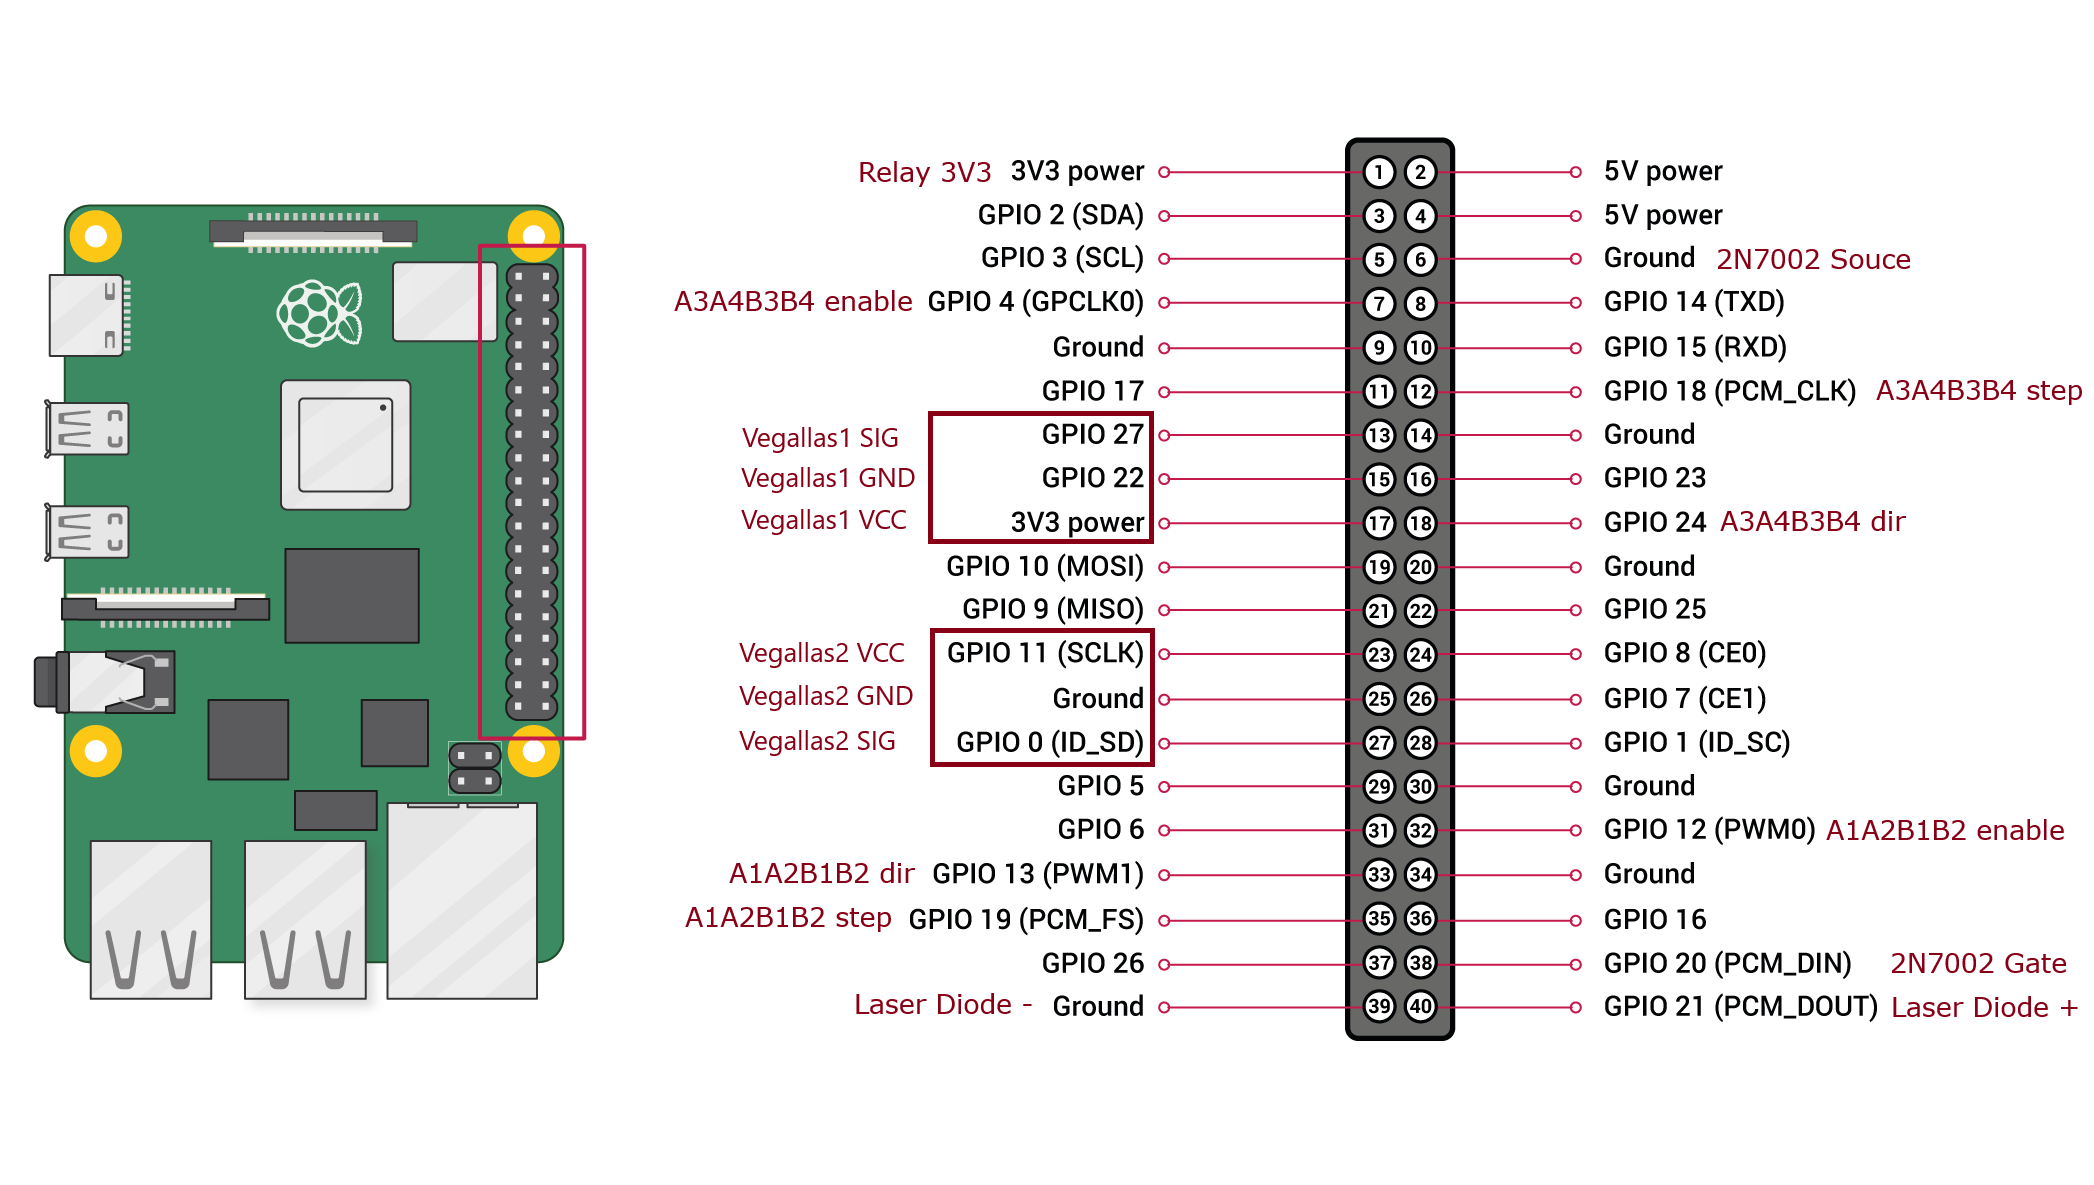
\includegraphics[width=1\linewidth]{elek_pinout}
	\caption{A Raspberry PI lábkiosztása \cite{raspberry4}}
	\label{fig:elek_pinout}
\end{figure}


A prototípus áramköre a \ref{fig:schematic} ábrán látható. A kereskedelemben kapható \textsl{Stepper Motor HAT} nagyban leegyszerűsítette a tervezés folyamatát, a segítségével nem kellett megterveznem a motorvezérlők áramkörét, illetve ezeknek az áramellátását. A \ref{fig:elek_pinout}.ábrán látható, motorokra vonatkozó jelölések szerinti GPIO lábakat a \textsl{Stepper Motor HAT} ugyan lefoglalja, de a kártya tetején lévő tüskesor ugyanúgy elérhető marad, így oda kell figyelnem, hogy ezeket a lábakat ne használjam. \\

\begin{figure}[h!]
	\centering
	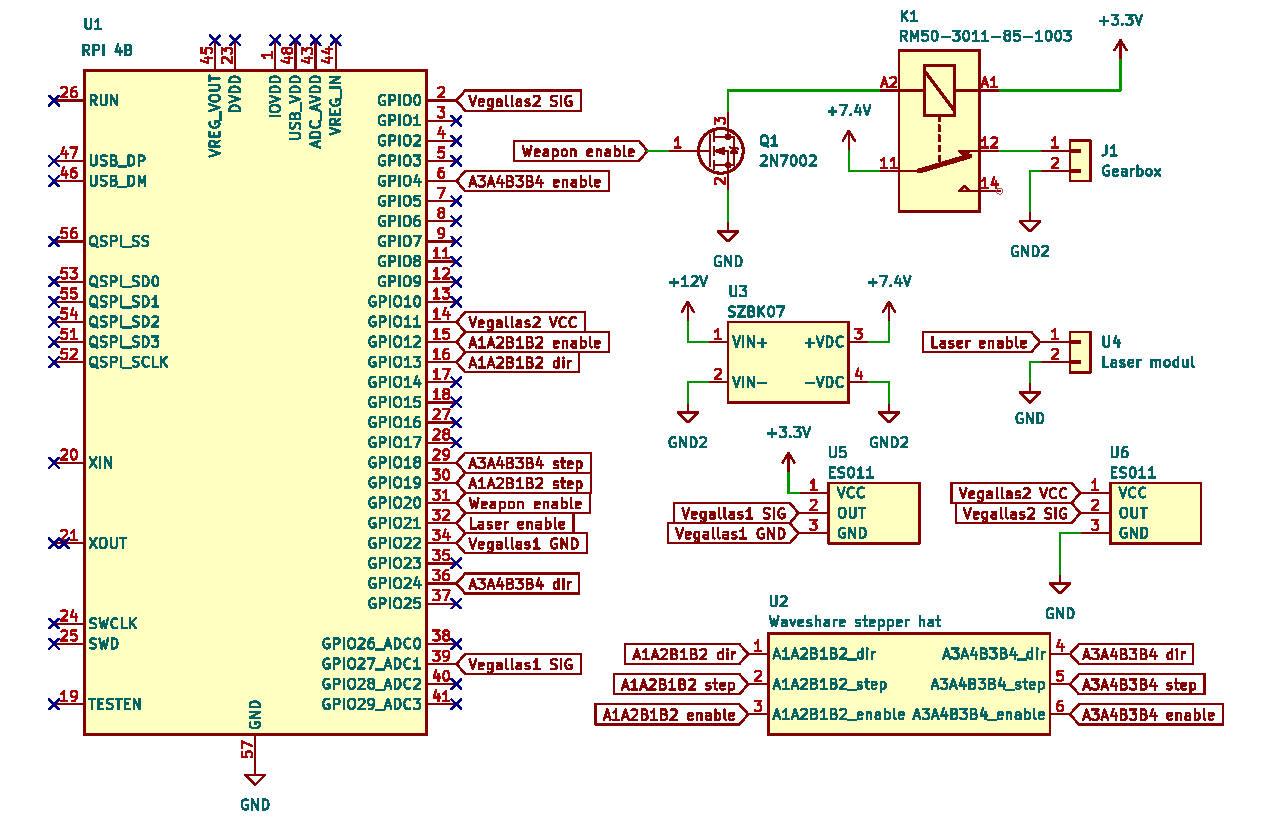
\includegraphics[width=1\linewidth]{schematic2}
	\caption{A prototípus sémarajza}
	\label{fig:schematic}
\end{figure}

Ahogy az ábrán látható, a végálláskapcsolók is a GPIO tüskesorra lettek csatlakoztatva. Az egyiknél a földet helyettesíti GPIO22 láb, a másiknál a 3.3 V-t helyettesíti a GPIO11. Azért kellett ezt a megoldást alkalmaznom, mert a kábel csatlakozója egyben van, nem különálló jumper tüskék.\\

A lézer közvetlenül a GPIO21 lábról működik. Eleinte aggódtam, hogy nem tud elegendő áramot szolgáltatni a dióda működtetéséhez, de szerencsére mégis. Ellenkező esetben ki kellett volna egészítenem az áramkört egy tranzisztorral. \\

A relé kapcsolásához viszont nem volt elegendő a GPIO láb által szolgáltatott áram, így azt egy tranzisztorral vezérlem. Amennyiben logikai magas jelet kap, a relé zárja a gearbox áramkörét, és az elkezd lőni.

Az eszköz sémarajza az alábbi ábrán látható:


\pagebreak

\section{Elektronikai alkatrészek}
\subsubsection*{Mikrovezérlő}
A mikrokontroller kiválasztásánál több opciót vizsgáltam, többek között az {Arduino}, az \textsl{STM-32} és a \textsl{Raspberry PI} modelleket. A követelmények a következőek voltak:

\begin{list}{$\bullet$}{}
	\item Legyen könnyen beszerezhető, mind anyagilag, mind elérhetőség szerint
	\item Megfelelő teljesítmény gépi látás algoritmusokhoz
	\item Elegendő számú GPIO kimenet
	\item Python programozási nyelve támogatása
	\item Ethernet port
\end{list}

Ahogy összehasonlítottam a különböző opciókat, körvonalazódott, hogy a \textsl{Raspberry PI} \cite{raspberry4} lesz a megfelelő megoldás. Az eszköz az \ref{fig:elek_raspberry4b}. ábrán látható. Először is egy gyakorlati szempont szerint, mégpedig hogy egy Raspberry PI 4B modell eredetileg is volt a tulajdonomban 4GB rammal. A gyártó hivatalos fórumán több felhasználó szerint ez már elegendő összetettebb gépi látás algoritmusok futtatására is. \cite{4gbforum} \\

\begin{figure}[h!]
	\centering
	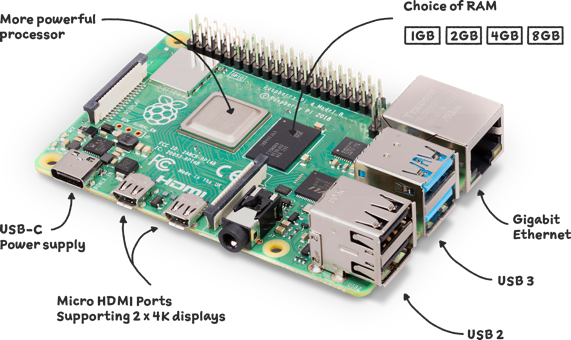
\includegraphics[width=0.5\linewidth]{elek_raspberry4b}
	\caption{Raspberry 4 model B \cite{raspberry4}}
	\label{fig:elek_raspberry4b}
\end{figure}

A kamera illesztése szintén különösen fontos a végtermék működése szempontjából, és ezen a területen magasan kiemelkedik a Raspberry a többi mikrovezérlő közül, mivel a gyártó magán a termékcsaládon belül ajánl több jó minőségű, könnyen beszerezhető kamera modult, amik illesztése már kiforrott az összes Raspberry-hez.\\

Ezentúl a \textsl{Raspberry PI} erősebb, mint a fentebb említett mikrokontrollerek. Linux rendszert futtat, és lehet rajta Python nyelven programozni, ami gépi látás, automatizálás projekteknél hatalmas előny. Számos ki-és bemenete van, ráadásul támogatja a \textsl{Bluetooth}, \textsl{Wi-Fi}, és gigabites \textsl{Ethernet} kapcsolatokat is, nem beszélve a rengeteg bővítő "kabátról", amiket lehet kapni hozzá. Ezek a termék továbbfejlesztését nagyban könnyítik, ráadásul kevesebb munkát kell a nyomtatott áramkör tervezésébe tenni.\\

\subsubsection*{Stepper Motor HAT \cite{stepperhat}}
A NEMA-17 léptetőmotorok vezérlésére több megoldás is létezik, elterjedtek a \textsl{A4988}, \textsl{TMC5160T} és \textsl{DRV8825} típusú vezérlők. Ezeket azonban vagy külön modulként lehet megvásárolni, vagy pedig SMD alkatrészként, ami mellé mindenképpen kell tervezni kiegészítő áramkört. \\

\begin{figure}[h!]
	\centering
	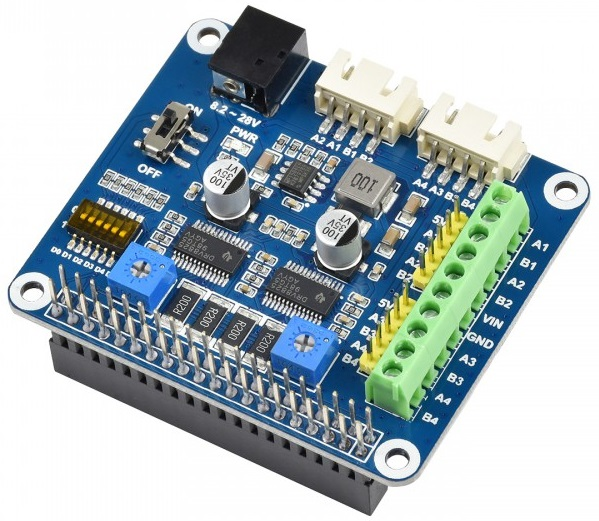
\includegraphics[width=0.4\linewidth]{elek_stepperhat}
	\caption{Waveshare Stepper HAT \cite{stepperhat}}
	\label{fig:elek_stepperhat}
\end{figure}

Azonban a \textsl{Waveshare} cég gyárt egy Raspberry Pi-kompatibilis modult, ami számomra rengeteg segítséget nyújtott. Ez egy külön áramkör, amit a Raspberry GPIO tüskesorára lehet illeszteni. Képes két \textsl{DRV8825} vezérlővel egyszerre kettő léptetőmotort vezérelni. A kártyán lévő kapcsolókkal könnyen lehet állítani külön motoronként a microsteppelést is, amennyiben szükség van rá egészen 1/32-ig. Szoftveresen is lehet állítani a microsteppelést, azonban ehhez forrasztani kellene a kártyára plusz ellenállásokat. A potméterekkel motoronként tudjuk állítani a maximális felvehető áramot, maximum 2.5 A-ig. A kártyán helyet kapott egy standard 5.5 mm-es csatlakozó is, amivel 8.2 V és 28 V közötti feszültséggel lehet táplálni az áramkört. Egy belső regulator chip segítségével a Raspberry PI-t is el lehet látni árammal, így egy tápegységgel tudom működtetni a teljes áramkört. A modulon több lehetőség is van csatlakoztatni a motorokat, akár sorkapoccsal, akár a léptetőmotorok szabvány csatlakozójával. Ezentúl lehetővé teszi a Raspberry PI GPIO lábainak elérését, csupán arra kell odafigyelni, melyikeket használja. Az eszközről a \ref{fig:elek_stepperhat}. ábrán látható illusztráció. Az eszköz el lett látva különböző biztonsági funkciókkal, pl. túláram védelemmel, magas hőmérséklet elleni védelemmel, illetve alulfeszültség lockout-tal. \\

A gyártó szintén elérhetővé tett illesztőszoftvereket több eszközre, több motortípusra, amit a későbbiekben én is tudtam használni.

\subsubsection*{Táp}

A prototípust két tápegységről működtetem. Az egyik a Raspberry PI, a léptetőmotorok és a szenzorok áramellátásáért, ez egy standard 5.5 mm-es csatlakozóval ellátott laptop töltő. 14.5 V tápfeszültséget és maximum 5 A áramot képes biztosítani, amely bőven elegendő a vezérlőelektronika ellátására. A másik táp egy \textsl{HP ps-3701-1} 12 V-os redundáns szervertáp 725 W teljesítménnyel. 

\subsubsection*{DCDC konverter}
A gearbox gyárilag 7.4 V-ról tud működni, tehát a kapott 12V-ot át kellett alakítani. Erre egy \textbf{SPX-20A} típusú DC-DC step-down konverted modult alkalmaztam. Ennek a maximum kimeneti árama 20A, maximum teljesítménye 300W. Elméletileg a gearbox felvett árama tüskeszerűen fellőhet 15A fölé, ami fölött már ventilátoros hűtés javasolt, de mivel ez nem lenne tartós, így én úgy döntöttem, ezt kihagyom. A kimeneti feszültséget és az áramkorlátot lehet állítani a kártyán található potméterekkel, de gyakorlatban csak a feszültséget állítottam. Minél nagyobb feszültséggel hajtom a gearboxot, annál gyorsabban pörög a motor, tehát annál nagyobb gyakorisággal lövi ki a golyókat. A gearbox és a táp kábeleit a kártyán található csavaros terminállal csatlakoztattam, maga a modul pedig a kereten kapott helyet, a Raspberry PI konzolján.

\subsubsection*{Kamera}
A rendszer által használt kamera egy \textsl{Raspberry Pi Camera Module 2} volt.\cite{raspberrycam} Ez a modul 8 MP-es \textsl{Sony IMX219} szenzorral rendelkezik, amivel 3266 x 2450 felbontású állóképet tud készíteni. Képes Full HD videót felvenni 30 fps-el, HD-t 60 fps-el, vagy 640x480 felbontást 90 fps-el. A modul a \ref{fig:elek_raspberrycam}. ábrán látható.

\begin{figure}[h!]
	\centering
	
\includegraphics[width=1\linewidth]{elek_raspberrycam}
	\caption{Raspberry Pi Camera Module 2 \cite{raspberrycam}}
	\label{fig:elek_raspberrycam}
\end{figure}

A kamera befoglaló mérete szerelési furatai és CSI portja megegyezik a többi Raspberry kamerával, így a továbbfejlesztés esetén könnyedén lehet őket cserélni.

\subsubsection*{Végálláskapcsoló}
A prototípus bekapcsolásánál fontos, hogy beálljon egy kezdőpozícióba, és ahhoz képest tudjuk viszonyítani a mozgását. Ezt én a két tengelyen 1-1 végálláskapcsolóval oldottam meg. Ezek a modulok könnyen szerelhetőek a 3D nyomtatott vázra, és az alapján adnak jelet, valami van-e az optokapu között. A Raspberry GPIO lábaira könnyedén lehet őket bekötni jumper kábelek segítségével.

\pagebreak

\section{Gyártás, forrasztás}
A projekthez egyedi nyomtatott áramkört nem kellett gyártatni, azonban egy kis forrasztást igényelt. A gearbox táp folyamatos működéséhez az alább látható módon kellet egy huzallal összeforrasztanom a padokat. Látható a 12V és GND-hez csatlakozó kábelek is, amiket szintén beforrasztottam a megfelelő helyre. Ezen a területen van lehetőség a továbbfejlesztésre, például egy 3D nyomtatott elemmel.\\

Ezentúl a kábeleket kellett forrasztanom, illetve a relé és a hozzá tartozó tranzisztor áramkörét. Ezek az alábbi képen láthatóak. Azokat a kábeleket, ahol nagyobb áram folyhat, és szerettem volna, hogy szerelhetőek legyenek, ott WAGO 221 összekötőkkel oldottam meg a csatlakozást.

\chapter{Szoftverfejlesztés}
A prototípus szoftverét kettéválasztottam a két működési mód szerint, az egyik a manuális vezérlést valósítja meg, a másik az automatikust. A kettő között lényeges különbségek vannak a prioritásokban. A kézi vezérlésnél a legfontosabb a valós idejű megjelenítés, és a minél gyorsabb reagálás a felhasználói parancsokra. Az automata működésnél a megjelenítés kevésbé fontos, viszont a képfelismerés és ez által a célpont követése kiemelkedő fontosságú.


\section{Használt Python modulok, eszközök}
\subsection*{OpenCV könyvtár \cite{opencv}}
Az \textbf{OpenCV} (Open Source Computer Vision Library) egy nyílt forráskódú könyvtár, amelyet eredetileg az Intel fejlesztett ki, és amelyet széles körben használnak a számítógépes látás (computer vision) és képfeldolgozás területén. Az OpenCV rendkívül sokoldalú eszközkészletet biztosít a képekkel és videókkal kapcsolatos különféle feladatok megoldásához, amelyet elsősorban C++-ban fejlesztettek ki, de támogat Python, Java, és MATLAB interfészeket is. A Python interfész különösen népszerű, mivel egyszerűsíti az OpenCV használatát gépi tanulási és mesterséges intelligencia-alkalmazásokban. A fő funkciói közé tartozik a képfeldolgozás, tárgy- és arcérzékelés, mozgáskövetés, valamint a 3D-s modellezés és képanalízis.\\

Az OpenCV architektúrája moduláris felépítésű, ami lehetővé teszi a különböző funkciók rugalmas használatát. A modulok között megtalálhatóak a képfeldolgozási, objektumfelismerési, gépi tanulási és 3D modellezési könyvtárak. A Pythonban a \code{cv2} könyvtárként importálható OpenCV API biztosítja a különböző funkciók egyszerű elérését, így akár néhány sor kóddal is gyors eredmény érhető el.\\

Többféle képformátumot támogat, például JPEG, PNG és BMP, és rendelkezik valós idejű video- és képadatok betöltésére szolgáló funkciókkal is, például a \code{VideoCapture} objektummal. Ez utóbbi lehetővé teszi, hogy közvetlenül kamerákból vagy videófájlokból dolgozzunk.\\

Az \textbf{OpenCV }használata igen elterjedt az iparban és a kutatásban is, többek között autonóm járművek, biztonsági rendszerek, gyártósori ellenőrző rendszerek, orvosi képalkotás és mobilalkalmazások terén. A könyvtár rugalmassága és széleskörű támogatása lehetővé teszi, hogy számos programozási és mérnöki területen is alkalmazható legyen, ahol képfeldolgozásra és gépi látásra van szükség.

\subsection*{Socket modul \cite{socket}}

Python \code{socket} modulja alacsony szintű hozzáférést biztosít a hálózati kommunikációhoz, lehetővé téve különböző típusú hálózati kapcsolatok létrehozását, beleértve az általam használt TCP-t és az UDP-t.\\

A \textbf{TCP} kapcsolat-orientált protokoll, amely biztosítja az adatok érkezési sorrendjét és helyességét. A \code{socket.SOCK\textunderscore STREAM} típust használjuk, ha TCP kapcsolatot szeretnénk létrehozni. A TCP kapcsolatok esetében a \code{connect()} függvény a kapcsolat kezdeti lépése, és a kliens-szerver kommunikáció folyamatosan fennmarad.\\

Az \textbf{UDP} kapcsolatnélküli protokoll, amely nem garantálja az adatok sorrendjét és integritását, viszont gyorsabb, mivel nincs szükség kapcsolatra. Az UDP kapcsolathoz a  \code{socket.SOCK\textunderscore DGRAM} típust használjuk, így a kliens és a szerver bármikor küldhet és fogadhat adatokat. Ideális valós idejű alkalmazásokhoz, ahol nem kritikus minden csomag megérkezése (pl. video streaming).\\

Mindkét típusnál a \code{send()}, \code{sendto()}, \code{recv()}, és \code{recvfrom()} függvények használhatók az adatok küldésére és fogadására.

\subsection*{Multiprocessing modul \cite{multiprocessing}}

A \textbf{multiprocessing} modul lehetővé teszi a Python számára, hogy párhuzamosan több folyamatot indítson el, ami segít a CPU-erőforrások jobb kihasználásában. A modul az operációs rendszer által kezelt különálló folyamatokat hoz létre, így azok külön memóriaterülettel rendelkeznek, és jobban teljesítenek többmagos processzorokon, mint a \textsl{threading} modul.\\ 

A \code{Process} osztály segítségével indíthatunk el új folyamatokat, amelyek egymástól függetlenül végrehajtanak egy adott funkciót. A modul támogatja az eseménykezelést, kommunikációs csatornákat (pl. \code{Queue}, \code{Pipe}) és szinkronizálást (pl. \code{Event}, \code{Lock}), amelyek segítségével a folyamatok egymással adatokat cserélhetnek és szinkronizálhatják működésüket.

\subsection*{Pygame modul \cite{pygame}}

A \textbf{pygame} egy multimédiás modul, amely elsősorban 2D játékok fejlesztésére alkalmas, de egyéb alkalmazásokkor is lehetőséget ad bemenetek kezeléséhez.\\

A \code{pygame.event.get()} függvény segítségével olvashatjuk le az egér- és billentyűzet-eseményeket, így például kattintások, gombnyomások és egérmozgások lekérdezése egyszerű. Az interaktív elemek kirajzolása és mozgatása egyszerű a \code{pygame.display.update()} és \code{pygame.draw} függvényekkel, amelyek lehetővé teszik grafikus objektumok megjelenítését a képernyőn. Magában foglalja a számítógépes grafikákat, a hang- és programkönyvtárakat, amiket a Python programozási nyelvre fejlesztettek ki. 

\subsection*{Pickle modul \cite{pickle}}
A \textbf{pickle} modul sorosítást és deszerializációt tesz lehetővé, azaz a Python-objektumok bináris formátumba alakítását és visszaalakítását.\\

A \code{pickle.dumps()} segítségével a Python-objektumokat bináris formátumba alakíthatjuk, amely lehetővé teszi azok egyszerű tárolását vagy átvitelét, például hálózaton keresztül. A \code{pickle.loads()} a bináris formátumú adatokat visszaalakítja eredeti Python-objektummá. A pickle használata előnyös lehet akkor, ha komplex adatszerkezeteket szeretnénk fájlban tárolni vagy hálózaton keresztül továbbítani.

\pagebreak

\section{Gépi látás}
A célpontfelismerés módszere volt az automata működés legfontosabb eleme. Elsősorban az OpenCV könyvtár különböző lehetőségeit vizsgáltam, ugyanis ez a legjobban kiforrott modul, amely könnyedén használható python programokban.

\subsection{Template matching \cite{templatematching}} \label{sec:soft_template}

A \textbf{Template Matching} (sablonillesztés) egy egyszerű, de hatékony módszer, amelyet statikus képekben keresett minták (sablonok) azonosítására használnak. Ez a módszer összehasonlít egy kisebb, előre meghatározott képrészletet (a sablont) a nagyobb képen található területekkel, és megkeresi a legjobban illeszkedő pozíciót.\\

\textbf{Működés:} Az OpenCV \code{cv2.matchTemplate()} függvényével kivitelezhető, amely végigfuttatja a sablont a célképen, és minden pixelpozíciónál egy hasonlósági pontszámot generál. A legmagasabb értékű pontszám mutatja az illeszkedés helyét.\\

\textbf{Előnyei:} Gyors és könnyen implementálható, különösen ismert méretű és orientációjú objektumok azonosításához.\\

\textbf{Korlátozások:} Gyengén teljesít forgatott, méretarányosan eltérő vagy eltorzult objektumoknál, valamint változó fényviszonyok mellett.

\subsection{Feature Matching \cite{featurematching}} \label{sec:soft_feature}

A \textsl{Feature Matching} (jellemzőpont-illesztés) egy kifinomultabb módszer a képjellemzők összehasonlítására és egyeztetésére. A módszer a két képben található pontokat (feature-ket) párosítja, ezáltal lehetővé teszi forgatásokkal, elforgatásokkal és méretarányokkal szembeni robusztus egyeztetést.

\textbf{Működés:} Először meghatározzuk a képen lévő fontos jellemzőpontokat (például élek, sarkok), amelyeket különböző detektorok (például SIFT, SURF vagy ORB) segítségével találhatunk meg. Ezután az \code{cv2.BFMatcher()} (Brute Force Matcher) vagy a \code{cv2.FlannBasedMatcher()} függvénnyel azonosítjuk a jellemzőpontokat.\\

\textbf{Előnyei:} Robusztus a forgatásokkal, skálázással és elmozdulásokkal szemben, így alkalmas tárgyak nyomon követésére és objektumok felismerésére különböző nézetekből.\\

\textbf{Korlátozások:} A nagy számítási igényű algoritmusok miatt lassabb lehet, különösen nagy méretű képeken.

\subsection{Target Tracking \cite{targettracking}} \label{sec:soft_target}

A \textsl{Target Tracking} (célkövetés) feladata egy mozgó objektum követése egy videófolyamon vagy valós idejű képforráson keresztül. Az OpenCV több nyomon követési algoritmust is biztosít, amelyek segítenek abban, hogy a kiválasztott objektumot stabilan követni tudjuk, még akkor is, ha változik a pozíciója vagy a környezeti fény.

Algoritmusok:
\begin{list}{-}{}
	\item Mean Shift: A \code{cv2.meanShift()} függvénnyel elérhető algoritmus egy adott objektum körüli eloszlás csúcsértékeit keresi, és folyamatosan frissíti a helyét.
	\item CamShift (Continuously Adaptive Mean Shift): \code{A cv2.CamShift()} algoritmus a Mean Shift továbbfejlesztett változata, amely figyelembe veszi az objektum méretének és alakjának változásait.
	\item Modern nyomkövetési algoritmusok: Az OpenCV 3.x-es és újabb verziói lehetővé teszik algoritmusok használatát, mint a KLT (Kanade-Lucas-Tomasi) nyomkövető, a CSRT és a MedianFlow, amelyek kifejezetten valós idejű és pontos követést biztosítanak.
\end{list}

\textbf{Előnyei:} Alkalmas valós idejű alkalmazásokhoz, mint például a videó megfigyelés vagy az autonóm rendszerek, ahol a cél folyamatosan mozgásban van.

\textbf{Korlátozások:} Bizonyos algoritmusok hajlamosak elveszteni a célpontot gyors mozgásoknál vagy hirtelen pozícióváltásoknál.
\subsection{Haar cascade \cite{haarcascade}} \label{sec:soft_haar}

A \textsl{Haar Cascade} módszer az egyik legelterjedtebb technika az objektumfelismerésre, különösen az arcfelismerésben. A gépi tanuláson alapuló módszer képes egy képben vagy videófolyamon objektumokat megtalálni azáltal, hogy mintákat ismer fel az előképzett adatok alapján.\\

\textbf{Működés:} A Haar-cascade egy többlépcsős osztályozó, amelyet sok pozitív és negatív mintából tanítanak be. \code{A cv2.CascadeClassifier()} osztály segítségével előre tanított modelleket, például arcokat, szemeket vagy különböző objektumokat kereshetünk.\\

\textbf{Gépi tanulás:} A módszer előnye, hogy nagyon hatékonyan képes felismerni az objektumokat. A gépi tanulás során a kimeneti modell jellemzőit úgy optimalizálják, hogy gyorsan tudja felismerni a keresett objektumokat még zajos vagy eltérő körülmények között is.\\

\textbf{Előnyei:} A Haar-cascade módszer jól használható olyan alkalmazásokhoz, ahol előre meghatározott objektumokat (például arcokat) kell azonosítani. Nagy előnye, hogy valós időben is képes futni.\\

\textbf{Korlátozások:} Hajlamos a pontatlan felismerésre, ha az objektumok perspektívája, megvilágítása vagy pozíciója jelentősen eltér az előképzett mintáktól. Alternatív megoldásként mélytanulási módszerek (például konvolúciós neurális hálózatok) használhatók az ilyen problémák javítására. \pagebreak



\section{A szoftver működése}
A rendszer két alapvető részből áll: egy számítógépből (PC), amely felhasználói interfészként szolgál az operátor számára, és egy Raspberry Pi-ből, amely a fegyverrendszer vezérlését és képátvitelét végzi. A két eszközön futó program között két folyamat kommunikál, két különböző porton: egy UDP protokoll alapú adatátvitel a videó küldéséhez, illetve egy TCP alapú a vezérlőparancsok fogadásához. \\

\subsection{A PC-n futó program működése}
A PC-s kód \code{main()} függvénye két külön folyamatot indít: egy videó-fogadó folyamatot és egy vezérlő-küldő folyamatot, melyek egy multiprocessing-eseményjelző (\code{stop\textunderscore event}) segítségével állnak meg szükség esetén. A két folyamat használ közös erőforrást, a \code{frame\textunderscore queue}-t, amelybe a videó-fogadó betölti a Raspberry-ből kapott képkockákat, a Pygame pedig felhasználja az a másik folyamatban. A felső szint folyamatábrája a \ref{fig:PC_main}. ábrán látható. 

\begin{figure}[h!]
	\centering
	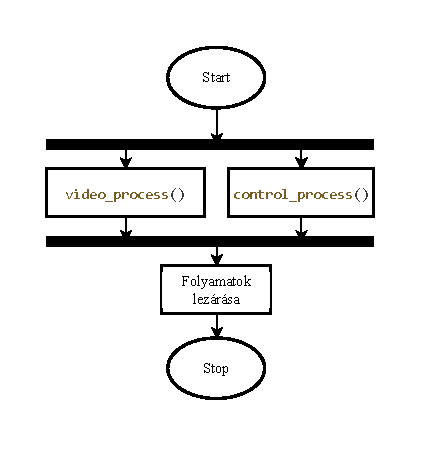
\includegraphics{PC_main}
	\caption{A PC-n futó program felső szintű folyamatábrája}
	\label{fig:PC_main}
\end{figure}

\subsubsection*{Videó-fogadó folyamat}

A videó-fogadó folyamat (\code{video\textunderscore receiver}) UDP-n keresztül kapja a képkockákat, amelyek a Raspberry Pi-ről érkeznek csomagokra bontva. A folyamat összegyűjti ezeket a csomagokat, majd a kép adatokat újraegyesíti és és betölti a \code{frame\textunderscore queue}-ba. Az UDP protokoll nagy sebességet tud elérni, de nem garantált a célba érés. A videó esetében azonban ez nem probléma, ha elveszik egy képkocka attól még értelmezhető marad a videó. A folyamat a következőképpen működik:

\begin{list}{$\bullet$}{}
	\item A folyamat egy UDP socketet (\code{video\textunderscore socket}) hoz létre a megadott porton.
	\item Egy ciklusban fogadja a képkockák csomagjait, minden egyes csomag egy fejlécet és a kép adatrészleteit tartalmazza.
	\item A fejléc alapján a folyamat azonosítja a csomagokhoz tartozó képkockát és azok sorrendjét. A bufferben gyűjtött csomagokat az összes részlet megérkezése után egyesíti.
	\item Az egyesített képkockát visszafejti (unpickling és JPEG dekódolás), majd a képre helyez egy célkeresztet a \code{cv2.line()} függvény alkalmazásával.
	\item A teljes képkockát behelyezi a \code{frame\textunderscore queue} sorba, a \code{.put()} metódussal.
\end{list}

A folyamatábra a \ref{fig:PC_videoreceiver}. ábrán látható.

\begin{figure}[h!]
	\centering
	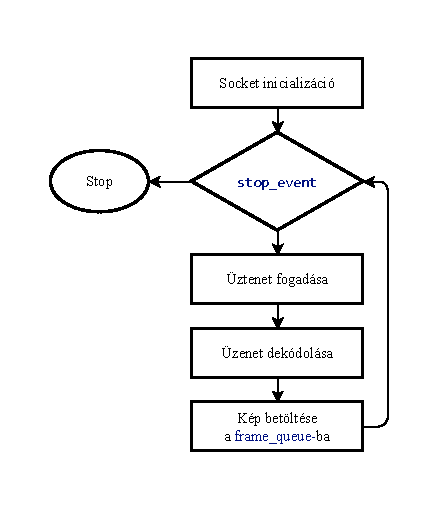
\includegraphics{PC_videoreceiver}
	\caption{A \code{video\textunderscore receiver} függvény folyamatábrája}
	\label{fig:PC_videoreceiver}
\end{figure}

\subsubsection*{Vezérlés-küldő folyamat}

A vezérlés-küldő folyamat (\code{control\textunderscore sender}) a felhasználó irányítási parancsait továbbítja a Raspberry Pi felé. A folyamat a Pygame könyvtár segítségével észleli az egér- és billentyűeseményeket, majd a megfelelő parancsokat TCP csomag formájában küldi a Raspberry Pi irányába. Ezentúl felelős a HUD megjelenítéséért, amiről a felhasználó le tudja olvasni a prototípus állapotát. A folyamat illusztrációja a \ref{fig:PC_controlsender}. ábrán látható.\\


\begin{figure}[h!]
	\centering
	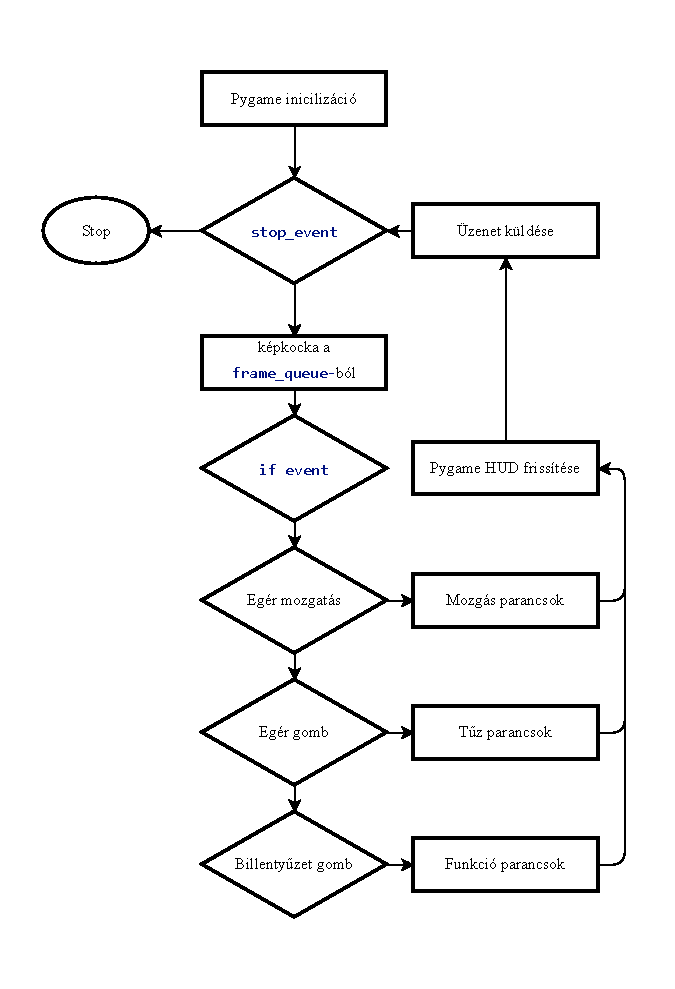
\includegraphics{PC_controlsender}
	\caption{A \code{control\textunderscore sender} függvény folyamatábrája}
	\label{fig:PC_controlsender}
\end{figure}

A felhasználó számára fontos, hogy minden információt le tudjon egyből olvasni a fegyver működéséről, így ezeket a PyGame ablakon megjelenítettem (\ref{fig:teszt_manual1}. ábra). Itt látható:

\begin{figure}[h!]
	\centering
	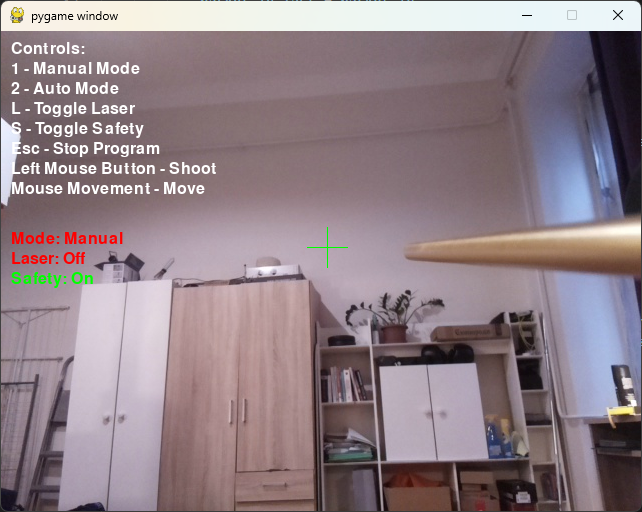
\includegraphics[width=0.5\linewidth]{teszt_manual2}
	\caption{Pygame HUD}
	\label{fig:teszt_manual1}
\end{figure}


\begin{list}{-}{}
	\item Használható parancsok és a hozzájuk rendelt gombok
	\item Milyen módban működik a rendszer
	\item Biztosítva van-e a rendszer
	\item Működik-e a lézer
\end{list}

A PyGame ablak háttere pedig az éppen utolsó képkocka, amit a videó-fogadó folyamat a \code{frame\textunderscore queue}-ba tett. A vizuális megjelenítés mellett a folyamat feladata a parancsok küldése, ezek a következőek lehetnek:

\begin{list}{-}{}
	\item Az egér mozgása esetén \code{MOVE} parancs az X és Y elmozdulási adatokkal, így irányítva a fegyver mechanikai elmozdulását.
	\item Az bal egérgomb lenyomásakor (\code{SHOOT\textunderscore START}, a felengedésekor \code{SHOOT\textunderscore STOP}) parancsot adhatunk ki, értelemszerűen a tüzelés megkezdésére és befejezésére.
	\item A billentyűzet gombjaival a lézert, (\code{LASERTOGGLE}) a biztosítást (\code{SAFETY}), illetve a működési módokat lehet állítani(\code{MANUALMODE} és \code{AUTOMODE}).
	\item Amikor a felhasználó az ESCAPE gombot megnyomja, a folyamat küld egy leállítási parancsot (\code{STOP}), majd befejezi működését.
\end{list}

A program a működési módtól függetlenül működik, mindig ugyanazokat az üzeneteket küldi el. A kliens programtól függ, hogyan értelmezi azokat.

\pagebreak

\subsection{A Raspberry Pi-n futó program működése}
A Raspberry Pi-n több folyamat is fut: Egy videó-küldő, egy vezérlés-fogadó, egy célpontfelismerő, illetve egy motormozgató. A közös erőforrások között szintén van egy \code{stop\textunderscore event} eseményjelző, amely minden folyamat megállításáért felelős. Ezentúl van a \code{frame\textunderscore queue} és a \code{pos\textunderscore queue}, amelyek tartalmazzák a képkockákat és a felismert célpont pozícióját. A \code{main()} függvény illusztrációja látható a \ref{fig:RPI_main}. ábrán.

\begin{figure}[h!]
	\centering
	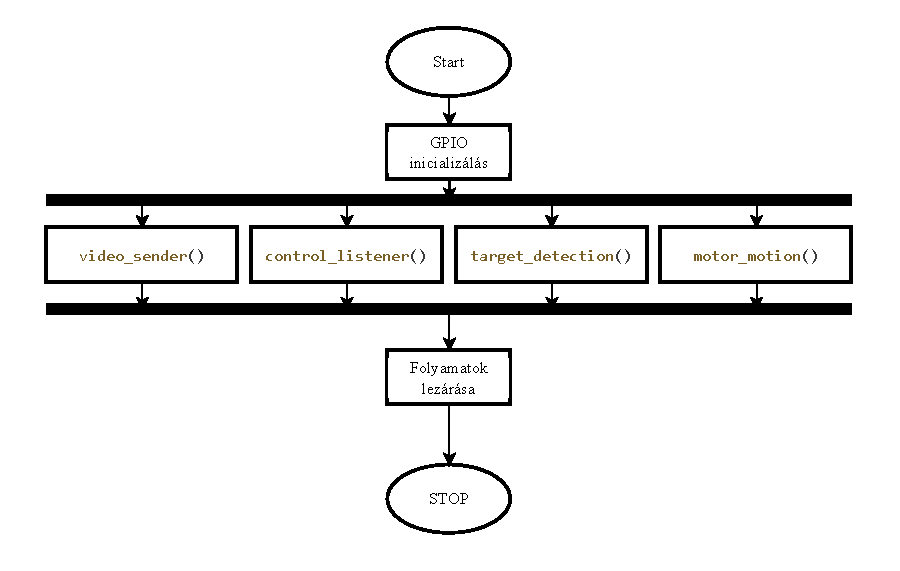
\includegraphics{RPI_main}
	\caption{A Raspberry PI-n futó program felső szintű folyamatábrája}
	\label{fig:RPI_main}
\end{figure}

\subsubsection*{Célfelismerő folyamat}

A \code{target\textunderscore detection()} folyamat felelős az arcok felismeréséért, és a helyzetük meghatározásához.

\begin{list}{-}{}
	\item A \code{cv2.CascadeClassifier()} függvénnyel betölti az előre betanított \textsl{haarcascade\textunderscore frontalface\textunderscore default.xml} modellt
	\item A \code{frame\textunderscore queue.get()} metódussal kiveszi az utolsó képkockát a sorból
	\item A \code{cv2.detectMultiScale()} megtalálja az arcokat a képkockán
	\item Méret szerint sorba rendezi az arcokat, és kiszámolja a legnagyobb pozícióját
	\item Betölti a pozíciót a sorba a \code{pos\textunderscore queue.put} metódussal
\end{list}

Ez a folyamat csak akkor fut, hogyha az \code{automode\textunderscore event()} flag be van állítva, tehát az eszköz automatikusan működik. A folyamat illusztrációja a \ref{fig:RPI_targetdetection}. ábrán látható

\begin{figure}[h!]
	\centering
	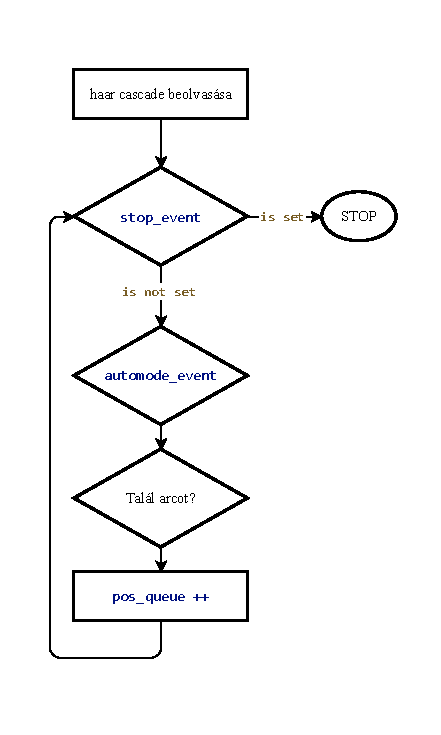
\includegraphics{RPI_targetdetection}
	\caption{A \code{target\textunderscore detection} függvény folyamatábrája}
	\label{fig:RPI_targetdetection}
\end{figure}


\subsubsection*{Vezérlés-fogadó folyamat}

A \code{control\textunderscore listener} folyamat először , a rendszer indításakor elvégzi a fegyver pozíciójának beállítását. A motorokat addig forgatja, amíg a végálláskapcsolók nem adnak jelet. Ezután pedig, miután tudjuk a pontos pozíció, visszaforgatja a fegyvert középre, és nullázza a \code{POSX} és \code{POSY} globális változókat. Ezután pedig TCP-n keresztül fogadja a PC-ről érkező irányítási parancsokat, és a megfelelő fizikai komponenseket működteti, majd a rendszer leállításakor újra középre állítja a fegyvert. A következő parancsokat tudja fogadni, attól függően, hogy melyik módban működik a prototípus. 

\begin{list}{-}{}
	\item A parancs típusa alapján (\code{MOVE}, \code{SHOOT\textunderscore START}, \code{SHOOT\textunderscore STOP},  \code{LASERTOGGLE}, \code{ STOP}) különböző műveleteket hajt végre.
	\item \code{MOVE} parancs esetén az X és Y elmozdulási értékek alapján irányítja a két DRV8825 motorvezérlő áramkört, így mozgatva a fegyvert az elvárt irányba.
	\item A lövésvezérlés (\code{SHOOT\textunderscore START} és \code{SHOOT\textunderscore STOP}) esetén aktiválja vagy deaktiválja a fegyver LED-jét.
	\item A lézerkapcsolás (\code{LASERTOGGLE}) a lézerdiódát ki- vagy bekapcsolja.
	\item Amennyiben \code{STOP} parancs érkezik, a folyamat leállítja a működését.
\end{list}

A függvény folyamatábrája a \ref{fig:RPI_controllistener}. ábrán látható.

\begin{figure}[h!]
	\centering
	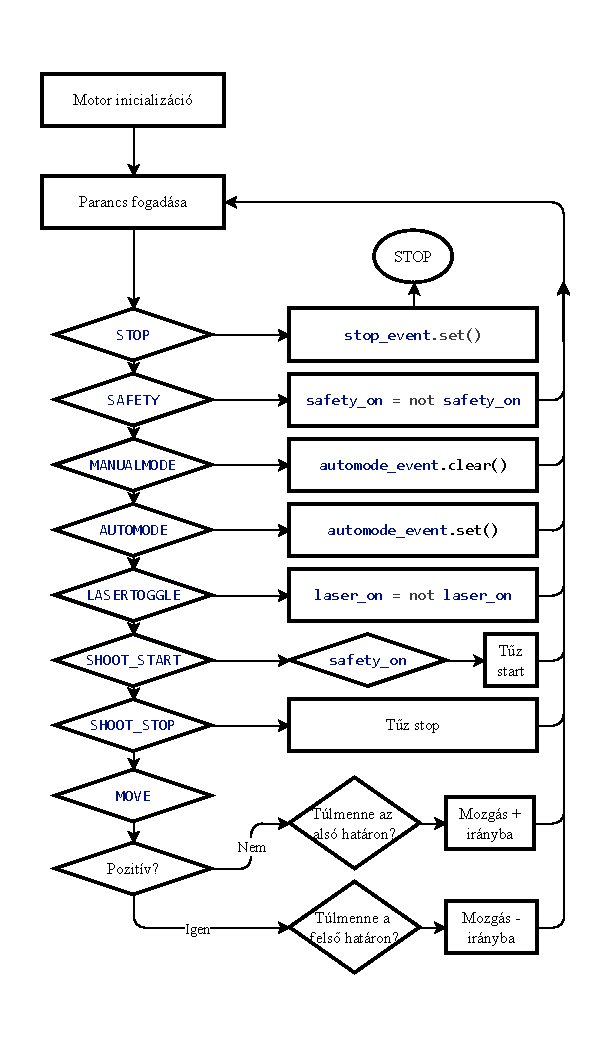
\includegraphics{RPI_controllistener}
	\caption{A \code{control\textunderscore listener} függvény folyamatábrája}
	\label{fig:RPI_controllistener}
\end{figure}


\begin{list}{-}{}
	\item \code{STOP} parancs esetén az \code{stop\textunderscore event}-et beállítja, ezzel leállítva az összes folyamatot
	\item \code{AUTOMODE} parancs esetén az \code{automode\textunderscore event}-et igazra állítja
	\item \code{MANUALMODE} parancs esetén az \code{automode\textunderscore event}-et hamisra állítja
	\item \code{MOVE} parancs esetén az X és Y elmozdulási értékek alapján irányítja a két motorvezérlőt, így mozgatva a fegyvert a megfelelő irányba.
	\item A (\code{SHOOT\textunderscore START} és \code{SHOOT\textunderscore STOP}) esetén aktiválja vagy deaktiválja a fegyvert. Aktiválni csak akkor lehet, ha a \code{safety\textunderscore on} hamis.
	\item A (\code{LASERTOGGLE}) a lézerdiódát ki- vagy bekapcsolja.
	\item Amennyiben \code{SAFETY} parancs érkezik, beállítja a \code{safety\textunderscore on} flag-et.
\end{list}

A végtelen ciklus ellenőrzi a \code{stop\textunderscore event} flag-et, és ha igaz lesz, akkor kilép belőle. Ekkor a \code{TurnStep()} fügvénnyel addig lép, amíg középen nem lesz a fegyver, valamint a lézert is lekapcsolja.

\begin{figure}[h!]
	\centering
	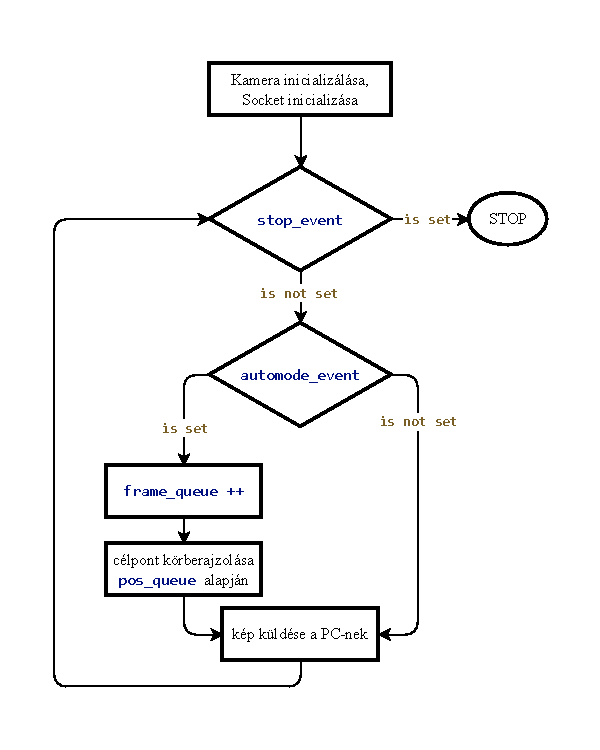
\includegraphics{RPI_videosender}
	\caption{A \code{video\textunderscore sender} függvény folyamatábrája}
	\label{fig:RPI_videosender}
\end{figure}

\subsubsection*{Videó-küldő folyamat}
A videó-küldő folyamat (\code{video\textunderscore sender}) a Raspberry Pi kamerájából érkező képet szerzi meg és osztja meg a PC-vel UDP kapcsolaton keresztül. A folyamat illusztrációja a \ref{fig:RPI_videosender}. ábrán látható.

\begin{list}{-}{}
	\item A kamerakép feldolgozása során a kód rögzíti az egyes képkockákat, amelyeket JPEG formátumba kódol és pickle segítségével tömörít.
	\item Amennyiben az \code{automode\textunderscore event} flag igaz, akkor beteszi a legutolsó képkockát a \code{frame\textunderscore queue}-ba, és a \code{pos\textunderscore queue} legutolsó elemei alapján húz egy téglalapot illeszt a képkockára, ezzel jelezve a talált arcot.
	\item Az adatok nagy mennyiségét figyelembe véve a képkockákat kisebb csomagokra bontja, amelyekhez megfelelő fejlécek tartoznak.
	\item A fejlécekben megtalálható a csomag azonosítója, amely segít a PC-n futó videó-fogadó folyamatnak a csomagok megfelelő sorrendbe állításában és összerakásában.
	\item A csomagokat a megadott IP-címre és portra küldi, és minden új képkockához új azonosítót rendel.
\end{list}

\begin{figure}[h!]
	\centering
	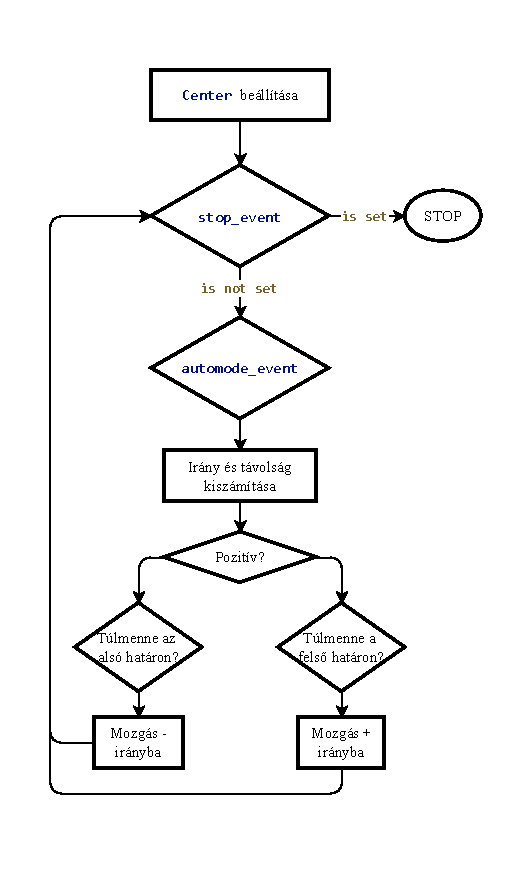
\includegraphics{RPI_motormover}
	\caption{A \code{motor\textunderscore motion} függvény folyamatábrája}
	\label{fig:RPI_motormover}
\end{figure}


\subsubsection*{Motormozgató folyamat}
A \code{motor\textunderscore motion()} folyamat azért felelős, hogy automata működés során mozgassa a motorokat, a kamera képe alapján. Azért gondoltam, hogy jobb így külön kezelni, mert az automata és kézi vezérlés mozgásának nagyon különböző a logikája. A folyamat működése a következőképpen működik:

\begin{list}{-}{}
	\item Kiolvassa a legutolsó pozíciót a \code{pos\textunderscore queue}-ből, majd a pozícióból és a középpont különbségéből kiszámítja a távolságot.
	\item Amennyiben a fegyver pozíciója a mozgásterületen belül van, a megfelelő irányba mozdul a távolsággal arányosan.
\end{list}

A motor csak akkor mozog, ha egy bizonyos értéknél nagyobb a távolság, így kerültem el, hogy folyamatosan rángatózzon az eszköz. Ez a folyamat is csak akkor fut, hogyha a \code{automode\textunderscore event} igaz. A folyamat illusztrációja a \ref{fig:RPI_motormover}. ábrán látható.


\chapter{Tesztelés}
A prototípus tesztelése több lépcsőben zajlott le, minden alkalommal több egységet hozzáadva. Az első a \textbf{hardver} tesztje volt, ahol a \textsl{motorok illesztése}, a \textsl{gearbox}, a \textsl{kamera} és a \textsl{szenzorok} megfelelő működését vizsgáltam, illetve a \textsl{kommunikációt} a Raspberry PI és a PC között. Miután a teszt alapján beállítottam a kamera optimális paramétereit és működésének algoritmusát, a következő teszt a különböző \textbf{célfelismerő algoritmusok} összevetése volt. Itt először egy statikus állványra került a kamera, és a képfelismerés \textsl{sebességét} és \textsl{megbízhatóságát} vizsgáltam. Miután kiválasztódott az optimális megoldás és elkészültek a 3D nyomtatott alkatrészek, kipróbáltam a célfelismerést a motorok mozgásával együtt is. Végezetül pedig \textbf{éles helyzetben} próbáltam ki a prototípust, ami tulajdonképpen céltáblára lövést jelentett. Ekkor vizsgáltam a szerkezet \textsl{stabilitását}, a \textsl{célfelismerést} nagyobb távolságokban, a tüzelési mechanizmus \textsl{megbízhatóságát} és \textsl{pontosságát}, illetve a \textsl{biztonsági funkciókat}.

\section{Elektronikai alkatrészek tesztje}
Ezen teszt során csatlakoztattam a kamerát a Raspberry PI megfelelő csatlakozójához, a NEMA-17 léptetőmotorokat pedig a Stepper Motor HAT csatlakozóihoz. Ezután a GPIO tüskesorhoz csatlakoztattam a lézer diódát, a relé megfelelő lábait, és a végálláskapcsolókat. A gearbox kábeleit összekötöttem a tápegységgel, legvégül pedig a Raspberry PI-t az ethernet porton keresztül a PC-hez csatlakoztattam, majd áram alá helyeztem. Először a Stepper Motor HAT gyártója által szolgáltatott illesztőprogramot próbáltam ki, átkonfigurálva a motor típusának és a microsteppelésnek megfelelően. Ezután a kamera gyári driver-ét teszteltem az \textsl{OpenCV} könyvtár használatával. Végül pedig konfiguráltam a GPIO lábakat, és teszteltem a lézer diódát, a végálláskapcsolókat és a relét. Ezzel együtt teszteltem a kezdetleges szoftvert és az eszközök közötti kommunikációt, ez magába foglalta a \textsl{Socket} és \textsl{Pygame} modulok különböző lehetőségeinek összevetését. A teszt összeállítása a \ref{fig:teszt_1}. ábrán látható. A teszt nem egy alkalommal zajlott le, inkább egy húzódó folyamatként, aminek során megtaláltam az optimális beállításokat a szoftverben.

\begin{figure}[h!]
	\centering
	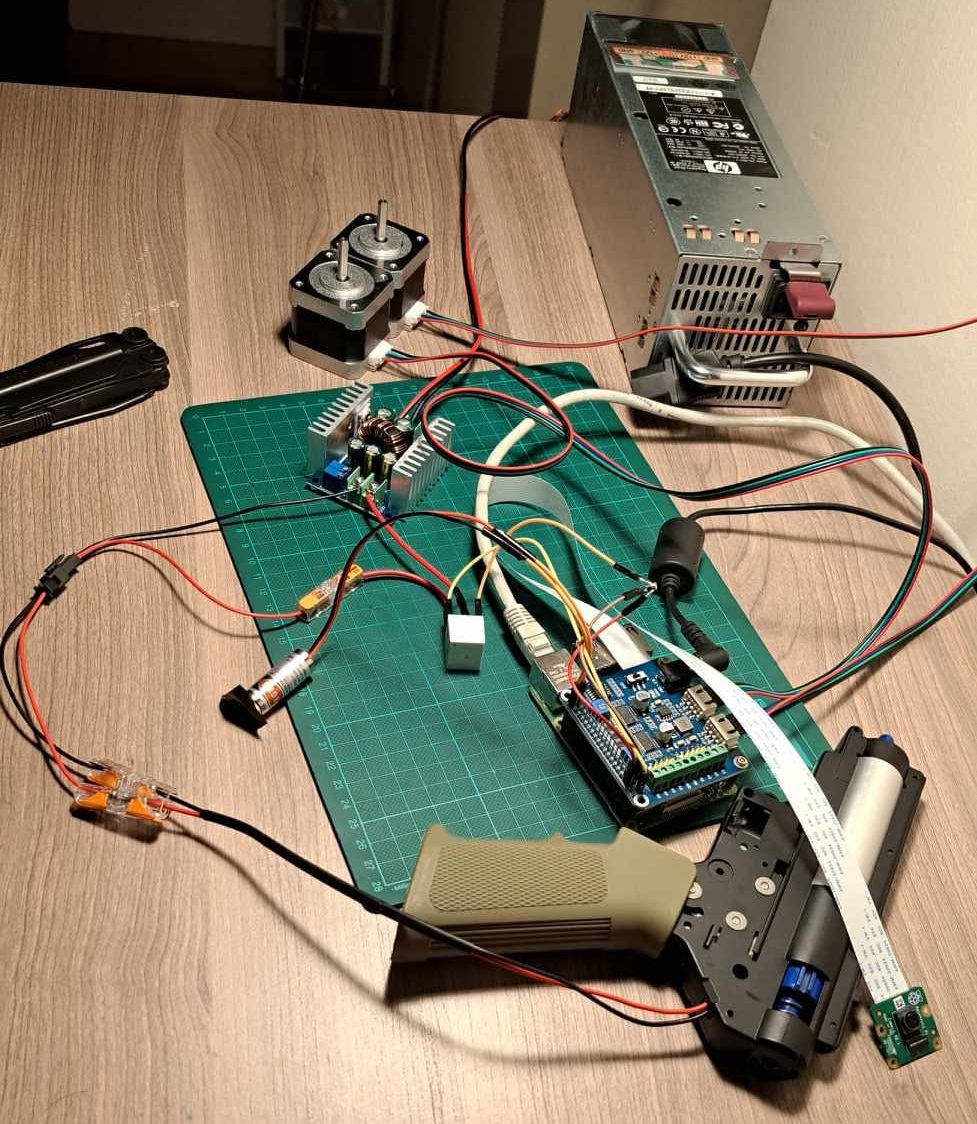
\includegraphics[width=0.5\linewidth]{teszt_1}
	\caption{Elektronikai alkatrészek teszt összeállítása}
	\label{fig:teszt_1}
\end{figure}


\pagebreak


\section{Képfelismerő algoritmusok tesztje}
A teszt összeállítása itt is ugyanaz volt, mint az előző bekezdésben, annyi különbséggel, hogy a kamerát felerősítettem egy állványra. A teszt során a kamera előtt mozgattam az aktuális célpontot, és a célfelismerés megbízhatóságát és sebességét vetettem össze. Először két olyan módszert vizsgáltam, ahol a célpont nem általános, hanem egy PNG képet vesz mintának, és ezt keresi a kamera által szolgáltatott képen, végül pedig egy betanított hálót.

\subsection*{Template Matching}
Erről a módszerről korábban a \ref{sec:soft_template}. bekezdésben volt szó bővebben. A \code{cv2.matchTemplate()} függvény megkeresi a képen a sablont, a \code{cv2.minMaxLoc()} pedig visszaadja a helyzetét, valamint az eredmény pontosságát. Az eredmény pontosságának megszabtam egy alsó határt, és azt változtattam a teszt során. Azt tapasztaltam, hogy ez a módszer nagyon érzékeny a célpont dőlésére és elfordulására, valamint a távolságára is, ezért nem tartottam megfelelő megoldásnak. Emellett minél nagyobb felbontású kép a sablon, a folyamat annál lassabb lesz.
\begin{figure}[h!]
	\centering
	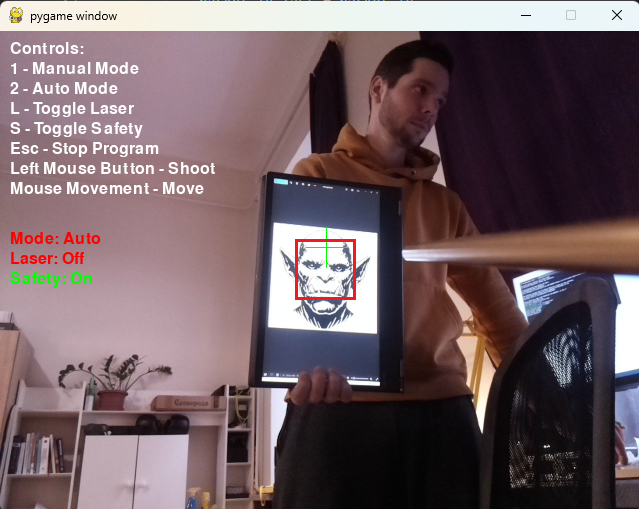
\includegraphics[width=0.8\linewidth]{teszt_auto2}
	\caption{Felismerő algoritmus tesztje}
	\label{fig:teszt_auto2}
\end{figure}
\pagebreak

\subsection*{Feature Matching és Target Tracking}
A feature matching elviekben jól kezeli a célpont torzulását, ezért ezzel kísérleteztem a későbbiekben. Az elképzelés az volt, hogy a feature matching megtalálja megbízhatóan a célpontot, majd a target tracking képes lesz gyorsan követni. A gyakorlatban, amennyiben egyszer megtalálta az algoritmus a célpontot, onnan tényleg pontosan tudta követni, azonban magával a felismeréssel voltak itt is a problémák. Nagyon megbízhatatlan volt, ha az érzékenységet lentebb állítottam, akkor fals pozitívot is mutatott, ha fentebb, akkor pedig nem találta meg a célpontot. A target tracking is csak akkor működött, ha a kamera egy helyben maradt. Ha már a motorok is mozogtak, akkor könnyedén elvesztette a célpontot.

\subsection*{Haar Cascade}
Az utolsó módszer, amit teszteltem, az a Haar Cascade és tanított neurális hálók használata volt. Ez az előzőekhez képest meglepően megbízható volt, a célpontot felismerte viszonylag távolról is, akár rossz fényviszonyok között is. A célpont kb 15 fokos dőlése esetén szintén felismerte azt, amit én megfelelőnek találtam. Ezzel a módszerrel folytattam a munkát. \\

Miután eldöntöttem, melyik módszerrel haladok tovább, kipróbáltam az algoritmust a fegyver mozgásával összhangban. Ennek módja az volt, hogy a kamera előtt egy laptopon mozgattam a sablon. Erről kép látható a \ref{fig:teszt_auto2}. ábrán.

\pagebreak

\begin{figure}[h!]
	\centering
	\includegraphics[width=1\linewidth]{teszt_setup2}
	\caption{Az éles teszt környezete}
	\label{fig:teszt_teszt_setup1}
\end{figure}

\begin{figure}[h!]
	\centering
	\includegraphics[width=1\linewidth]{teszt_setup1}
	\caption{Az éles teszt környezete}
	\label{fig:teszt_teszt_setup2}
\end{figure}

\pagebreak

\section{Éles teszt}
A tesztet egy jól megvilágított tanteremben végeztem. Az eszköz egy stabil padon állt, a célpont pedig 5 méterrel előtte, és kb. fél méterrel fölötte. A célpont a \ref{fig:teszt_teszt_setup2}. ábrán látható.\\

A teszt során a manuális működési móddal kezdtem, azon belül a fegyver kalibrálásával. Először azt tapasztaltam, hogy a kamera képének a közepe nem ott van, ahova a fegyver csöve mutat. Ezért a célkeresztet addig mozgattam a képen, amíg oda nem mutatott, ahova a fegyver ténylegesen lőtt. Ezután a rendszer nagy pontossággal tudott lőni, tulajdonképpen az összes leadott lövés a hibahatáron belül volt. A lézer irányzékot azonban nem tudtam pontosan beállítani, 5 méteren nagyjából 10-15 cm-t téved. A következő ábrákon látható a teszt eredménye. 5-ös sorozatokban tüzeltem, mindig a cél közepére irányítva a kamera célkeresztjét. \\

A következő teszt az arcfelismerés, és a követés funkció tesztje volt. A körülmények ugyanazok maradtak, és szintén 5 m-re volt a célpont. A teszt során egy kolléga tartotta a kinyomtatott arcképet, és mozgatta, változtatva a sebességet és irányt. Természetesen a gearbox nem volt áram alatt, és a kolléga is viselt védőszemüveget. Azt tapasztaltam, hogy a fegyver körülbelül a sétáló ember sebességét tudja követni 5 m távolságban, és igen pontosan be tudja célozni. A tesztkörnyezet a \ref{fig:teszt_teszt_setup1}. és \ref{fig:teszt_teszt_setup2}. ábrákon látható.

Összességében elmondható, hogy a beállított célkereszttel, 5 méterről igen pontos eredmények születtek. 4 leadott sorozat során 5-5 golyót lőttem ki, az eredmények az alábbi ábrán láthatóak:

\begin{figure}[h!]
	\centering
	\includegraphics[width=0.6\linewidth]{teszt_eredmenyek}
	\caption{Az éles teszt eredményei}
	\label{fig:teszt_eredmenyek}
\end{figure}
\chapter{Hibák, észrevételek}

A prototípus fejlesztés során számos helyen vétettem kisebb-nagyobb hibákat, amiket súlyosságuktól függően vagy javítani kellett, vagy valahogy kikerülni. Az első, amit meg szeretnék említeni, az a \textbf{tár kialakítása} volt. Nem voltam elég körültekintő, és anélkül terveztem meg a tárat, hogy megnéztem volna, az eredeti fegyverekben hogyan működik. Ennek eredménye lett a nagy kapacitású tár, aminek elméletben folyamatosan kéne adagolni a golyókat, de a gyakorlatban a szűkítésnél minden esetben elakad. Ezzel a kialakítással egyet sem sikerült tüzelni, így újra kellett tervezni a teljes tárat. Miután jobban megvizsgáltam az eredeti fegyvert, láttam, hogy a golyók egyesével sorakoznak minden esetben, ezzel gátolva az elakadást. Miután hasonlóan megterveztem az új tárat, már megbízhatóan működött, habár kisebb kapacitással, így ezt a hibát sikerült kijavítani.\\

A következő, egy szintén mechanikai természetű hiba, a \textbf{lézer modul és a kamera rögzítése}. Egyik sem állítható, és ha eredetileg nem egy pontra néznek a fegyver csövével, akkor tulajdonképpen a hiba maradandó lesz. Ez így is lett, de a kamera eltérését még a célkereszt állításával tudtam orvosolni. A lézer modul maradandóan pár fokkal félre áll, ezt sajnos el kellett fogadnom.\\

A projekt elektronikai részénél is van, amit máshogy csinálnék, ha újrakezdeném. Az első koncepcióterveknél még nem néztem utána, mekkora áramot képes felvenni a gearbox. Úgy gondoltam, hogy egy átlagos 12V-os laptoptöltőről is tud majd működni a rendszer. Így igen meglepődtem, mikor utánanéztem, mekkora teljesítményre van szüksége. Az eredmény így az lett, hogy egy külön tápot kellet adnom csak a gearbox működtetésére, ami igen kényelmetlen. Valószínűleg az lenne helyette egy jó megoldás, ha tervezek egy külön nyomtatott áramkört, amely képes arra, hogy töltsön egy akkumulátort a fegyveren. Így a gearbox arról működne, akár csak egy módosítatlan fegyveren, működésen kívül pedig a Raspberry PI tápjáról töltődne. 
\chapter{Továbbfejlesztési lehetőségek}
\textbf{Erősebb szerkezet:} Az egyik egyértelmű fejlesztési lehetőség a jobb minőségű alkatrészek használata. Elsősorban a fogaskerekekre gondolok, amelyeket ha nem 3D nyomtatással gyártottam volna, hanem valamilyen nagy pontosságú folyamattal, akkor a szerkezet nem csak csendesebb, de precízebb is lehetne.\\

\textbf{Jobb kamera:} A Raspberry PI Camera 2 megfelelő minőséggel rendelkezik arra, hogy ezt a prototípust használni tudjam vele. Azonban ha távolabbi célpontokat kellene keresni, akkor egy optikai zoom mindenképpen szükséges lenne.\\

\textbf{Vezeték nélküli működés:} A tápellátás és a kommunikáció vezeték nékülivé tétele magában hordozna új kihívásokat, például be kellene építeni egy nagyobb teljesítmény akkumulátort, illetve a vezeték nélküli kapcsolatok rendszerint lassabbak, mint a vezetékesek. Ellenben ha az eszköz célját tekintem, a távolsági operálás lenne a természetes fejlesztési irány, ahol a felhasználó akár egy másik épületből is képes lenne irányítani a fegyvert.\\

\textbf{Mozgás:} És ha már vezetékek nélkül képes működni az eszköz, akkor a következő lépés az lenne, hogy mozogni tudjon, például lánctalpak segítségével. Ez is szintén új kihívásokat jelent, de az eszköz többi részéhez képest már nem lenne nagyon bonyolult megvalósítani.\\

\textbf{Radar, távolságérzékelő:} Az eszköz következő verziójába kerülhetne akár radar is. A hasonló eszközök modern felhasználása leginkább légvédelmet jelent, azon belül drónok lelövését. Ezt vizuálisan nehézkes lehet érzékelni, hiszen igen távol is lehetnek, és kicsi a keresztmetszetük. Egy radar beépítése azonban megkönnyítené az észlelést. A távolságérzékelő pedig egyrészt több információt szolgáltat a célpontról, másrészt pedig nagy távolságoknál már számolni kell a lövedék ballisztikájával is, tehát hogy esik.

\chapter{Konklúziók}
Összességében véve magabiztosan jelentem ki, hogy a projekt sikerrel járt. A két félév alatt, amíg ezzel a feladattal foglalkoztam, amellett, hogy az elméleti ismereteimet a gyakorlatban is kipróbálhattam, rengeteg hasznos új tudást is szereztem. Közelebbről megismerkedtem a \textbf{3D nyomtatás} technológiájával, a \textbf{gépi látás} eszközeivel, illetve számos hasznos \textbf{Python} könyvtárral is. Most már van gyakorlatom a \textbf{Raspberry PI} alapú rendszerek fejlesztésében, ami a későbbi karrierem mellett a hobbi projektjeimben is előny lesz.\\

Elkészítettem a prototípust, amire vállalkoztam: az eszköz magabiztosan és stabilan képes mozogni, fürgén követi a felhasználó által adott parancsokat, és önálló célfelismerésre is alkalmas. A tüzelés is zökkenőmentesen működik, a lövedék nem akad el a tárban. Mindemellett meglepően pontos. Az biztonsági funkció, amikkel elláttam az eszközt, biztosítják, hogy olyan célpont ne legyen lelőve, akit az operátor nem szándékozott eltalálni. \\

A projekt teljes egészében bárki által elérhető a \textsl{GitHubon}, ugyanis szeretném, ha más is reprodukálni tudja, ha hasonló érdeklődéssel rendelkezik. Ezzel a gondolattal írtam a dokumentációt is, amiben próbáltam részletesen kitérni a megtett lépésekre, gondolatok hátterére.\\

A projektet valamilyen formában mindenképpen szeretném folytatni, akár egyedül, akár többedmagammal. Számos fejlesztési lehetőség maradt a prototípusban, és úgy gondolom több munkával, a most megszerzett tapasztalatokat bevetve, egy egészen kiforrott terméket készíthetünk el, amire talán mások is felfigyelnek.\\

Ha egy fontos konklúzió le szeretnék vonni így a feladatom végén, az az, hogy mindenképpen érdemes volt olyan feladatot választani amiben a technikai kihívás mellett van személyes motiváció is. Nem csak egy elvégzendő feladatként tekintettem a dolgozatra, hanem őszintén érdekelt a sorsa, és ezért a rengeteg tanulás mellett kijelenthetem, hogy élveztem is foglalkozni a projekttel. Úgy gondolom, a diplomamunkám egy méltó lezárása lesz az egyetemi tanulmányaimnak. 


%%----------------------------------------------------------------------------
\chapter{\LaTeX-eszközök}
\label{sec:LatexTools}
%----------------------------------------------------------------------------
\section{A szerkesztéshez használatos eszközök}
%----------------------------------------------------------------------------
Ez a sablon TeXstudio 2.8.8 szerkesztővel készült. A TeXstudio egy platformfüggetlen, Windows, Linux és Mac OS alatt is elérhető \LaTeX-szerkesztőprogram számtalan hasznos szolgáltatással (\refstruc{fig:TeXstudio}). A szoftver ingyenesen letölthető\footnote{A TeXstudio hivatalos oldala: \url{http://texstudio.sourceforge.net/}}.

\begin{figure}[!ht]
\centering
\includegraphics[width=150mm, keepaspectratio]{figures/TeXstudio.png}
\caption{A TeXstudio \LaTeX-szerkesztő.}
\label{fig:TeXstudio}
\end{figure}

A TeXstudio telepítése után érdemes még letölteni a magyar nyelvű helyesírásellenőrző-szótárakat hozzá. A TeXstudio az OpenOffice-hoz használatos formátumot tudja kezelni. A TeXstudio beállításainál a \verb+General+ fülön a \verb+Dictionaries+ résznél tudjuk megadni, hogy melyik szótárat használja.

Egy másik használható Windows alapú szerkesztőprogram a LEd\footnote{A LEd hivatalos oldala: \url{http://www.latexeditor.org/}} (LaTeX Editor), a TeXstudio azonban stabilabb, gyorsabb, és jobban használható.

%----------------------------------------------------------------------------
\section{A dokumentum lefordítása Windows alatt}
%----------------------------------------------------------------------------
A TeXstudio és a LEd kizárólag szerkesztőprogram (bár az utóbbiban DVI-nézegető is van), így a dokumentum fordításához szükséges eszközöket nem tartalmazza. Windows alatt alapvetően két lehetőség közül érdemes választani: MiKTeX (\url{http://miktex.org/}) és TeX Live (\url{http://www.tug.org/texlive/}) programcsomag. Az utóbbi működik Mac OS X, GNU/Linux alatt és Unix-származékokon is. A MiKTeX egy alapcsomag telepítése után mindig letölti a használt funkciókhoz szükséges, de lokálisan hiányzó \TeX-csomagokat, míg a TeX Live DVD ISO verzóban férhető hozzá. Ez a dokumentum TeX Live 2008 programcsomag segítségével fordult, amelynek DVD ISO verziója a megadott oldalról letölthető. A sablon lefordításához a disztribúcióban szereplő \verb+magyar.ldf+ fájlt a \verb+http://www.math.bme.hu/latex/+ változatra kell cserélni, vagy az utóbbi változatot be kell másolni a projekt-könyvtárba (ahogy ezt meg is tettük a sablonban) különben anomáliák tapasztalhatók a dokumentumban (pl. az ábra- és táblázat-aláírások formátuma nem a beállított lesz, vagy bizonyos oldalakon megjelenik alapértelmezésben egy fejléc). A TeX Live 2008-at még nem kell külön telepíteni a gépre, elegendő DVD-ről (vagy az ISO fájlból közvetlenül, pl. DaemonTools-szal) használni.

Ha a MiKTeX csomagot használjuk, akkor parancssorból a következő módon tudjuk újrafordítani a teljes dokumentumot:

\begin{lstlisting}[language=bash,frame=single,float=!ht]
$ texify -p thesis.tex
\end{lstlisting}

A \verb+texify+ parancs a MiKTex programcsomag \verb+miktex/bin+ alkönyvtárában található. A parancs gondoskodik arról, hogy a szükséges lépéseket (fordítás, hivatkozások generálása stb.) a megfelelő sorrendben elvégezze. A \verb+-p+ kapcsoló hatására PDF-et generál. A fordítást és az ideiglenes fájlok törlését elvégezhetjük a sablonhoz mellékelt \verb+manual_build.bat+ szkript segítségével is.

A \TeX-eszközöket tartalmazó programcsomag binárisainak elérési útját gyakran be kell állítani a szerkesztőprogramban, például TeXstudio esetén legegyszerűbben az \verb+Options / Configure TeXstudio... / Commands+ menüponttal előhívott dialógusablakban tehetjük ezt meg.

A PDF-\LaTeX~használata esetén a generált dokumentum közvetlenül PDF-formátumban áll rendelkezésre. Amennyiben a PDF-fájl egy PDF-nézőben (pl. Adobe Acrobat Reader vagy Foxit PDF Reader) meg van nyitva, akkor a fájlleírót a PDF-néző program tipikusan lefoglalja. Ilyen esetben a dokumentum újrafordítása hibaüzenettel kilép. Ha bezárjuk és újra megnyitjuk a PDF dokumentumot, akkor pedig a PDF-nézők többsége az első oldalon nyitja meg a dokumentumot, nem a legutóbb olvasott oldalon. Ezzel szemben például az egyszerű és ingyenes \textcolor{blue}{Sumatra PDF} nevű program képes arra, hogy a megnyitott dokumentum megváltozását detektálja, és frissítse a nézetet az aktuális oldal megtartásával.

%----------------------------------------------------------------------------
\section{Eszközök Linuxhoz}
%----------------------------------------------------------------------------
Linux operációs rendszer alatt is rengeteg szerkesztőprogram van, pl. a KDE alapú Kile jól használható. Ez ingyenesen letölthető, vagy éppenséggel az adott Linux-disztribúció eleve tartalmazza, ahogyan a dokumentum fordításához szükséges csomagokat is. Az Ubuntu Linux disztribúciók alatt például legtöbbször a \verb+texlive-*+ csomagok telepítésével használhatók a \LaTeX-eszközök. A jelen sablon fordításához szükséges csomagok (kb. 0,5 GB) az alábbi paranccsal telepíthetők:

\begin{lstlisting}[language=bash,morekeywords={sudo,apt\-get},alsoletter={-},breaklines=true]
$ sudo apt-get install texlive-latex-extra texlive-fonts-extra texlive-fonts-recommended texlive-xetex texlive-science
\end{lstlisting}

Amennyiben egy újabb csomag hozzáadása után hiányzó fájlra utaló hibát kapunk a fordítótól, telepítenünk kell az azt tartalmazó TeX Live csomagot. Ha pl. a \verb+bibentry+ csomagot szeretnénk használni, futtassuk az alábbi parancsot:

\begin{lstlisting}[language=bash,morekeywords={apt\-cache},alsoletter={-},breaklines=true]
$ apt-cache search bibentry
texlive-luatex - TeX Live: LuaTeX packages
\end{lstlisting}

Majd telepítsük fel a megfelelő TeX Live csomagot, jelen esetben a `texlive-lualatex`-et. (Egy LaTeX csomag több TeX Live csomagban is szerepelhet.)

Ha gyakran szerkesztünk más \LaTeX dokumentumokat is, kényelmes és biztos megoldás a teljes TeX Live disztribúció telepítése, ez azonban kb. 4 GB helyet igényel.

\begin{lstlisting}[language=bash,morekeywords={sudo,apt\-get},alsoletter={-},breaklines=true]
sudo apt-get install texlive-full
\end{lstlisting}

%%----------------------------------------------------------------------------
\chapter{A dolgozat formai kivitele}
%----------------------------------------------------------------------------
Az itt található információk egy része a BME VIK Hallgatói Képviselet által készített ,,Utolsó félév a villanykaron'' c. munkából lett kis változtatásokkal átemelve. Az eredeti dokumentum az alábbi linken érhető el: \url{http://vik.hk/hirek/diplomafelev-howto-2015}.

%----------------------------------------------------------------------------
\section{A dolgozat kimérete}
%----------------------------------------------------------------------------
Szakdolgozat esetében minimum 30, 45 körüli ajánlott oldalszám lehet az iránymutató. De mindenképp érdemes rákérdezni a konzulensnél is az elvárásokra, mert tanszékenként változóak lehetnek az elvárások.

Mesterképzésen a Diplomatervezés 1 esetében a beszámoló még inkább az Önálló laboratóriumi beszámolókhoz hasonlít, tanszékenként eltérő formai követelményekkel, -- egy legalább 30 oldal körüli dolgozat az elvárt -- és az elmúlt fél éves munkáról szól. De egyben célszerű, ha ez a végleges diplomaterv alapja is. (A végleges 60-90 oldal körülbelül a hasznos részre nézve)


%----------------------------------------------------------------------------
\section{A dolgozat nyelve}
%----------------------------------------------------------------------------
Mivel Magyarországon a hivatalos nyelv a magyar, ezért alapértelmezésben magyarul kell megírni a dolgozatot. Aki külföldi posztgraduális képzésben akar részt venni, nemzetközi szintű tudományos kutatást szeretne végezni, vagy multinacionális cégnél akar elhelyezkedni, annak célszerű angolul megírnia diplomadolgozatát. Mielőtt a hallgató az angol nyelvű verzió mellett dönt, erősen ajánlott mérlegelni, hogy ez mennyi többletmunkát fog a hallgatónak jelenteni fogalmazás és nyelvhelyesség terén, valamint -- nem utolsó sorban -- hogy ez mennyi többletmunkát fog jelenteni a konzulens illetve bíráló számára. Egy nehezen olvasható, netalán érthetetlen szöveg teher minden játékos számára.

%----------------------------------------------------------------------------
\section{A dokumentum nyomdatechnikai kivitele}
%----------------------------------------------------------------------------
A dolgozatot A4-es fehér lapra nyomtatva, 2,5 centiméteres margóval (+1~cm kötésbeni), 11--12 pontos betűmérettel, talpas betűtípussal és másfeles sorközzel célszerű elkészíteni.

Annak érdekében, hogy a dolgozat külsőleg is igényes munka benyomását keltse, érdemes figyelni az alapvető tipográfiai szabályok betartására~\cite{Jeney}.

%% !TeX spellcheck = hu_HU
% !TeX encoding = UTF-8
% !TeX program = xelatex
%----------------------------------------------------------------------------
\chapter{A \LaTeX-sablon használata}
%----------------------------------------------------------------------------

Ebben a fejezetben röviden, implicit módon bemutatjuk a sablon használatának módját, ami azt jelenti, hogy sablon használata ennek a dokumentumnak a forráskódját tanulmányozva válik teljesen világossá. Amennyiben a szoftver-keretrendszer telepítve van, a sablon alkalmazása és a dolgozat szerkesztése \LaTeX-ben a sablon segítségével tapasztalataink szerint jóval hatékonyabb, mint egy WYSWYG (\emph{What You See is What You Get}) típusú szövegszerkesztő esetén (pl. Microsoft Word, OpenOffice).

%----------------------------------------------------------------------------
\section{Címkék és hivatkozások}
%----------------------------------------------------------------------------
A \LaTeX~dokumentumban címkéket (\verb+\label+) rendelhetünk ábrákhoz, táblázatokhoz, fejezetekhez, listákhoz, képletekhez stb. Ezekre a dokumentum bármely részében hivatkozhatunk, a hivatkozások automatikusan feloldásra kerülnek.

A sablonban makrókat definiáltunk a hivatkozások megkönnyítéséhez. Ennek megfelelően minden ábra (\emph{figure}) címkéje \verb+fig:+ kulcsszóval kezdődik, míg minden táblázat (\emph{table}), képlet (\emph{equation}), fejezet (\emph{section}) és lista (\emph{listing}) rendre a \verb+tab:+, \verb+eq:+, \verb+sec:+ és \verb+lst:+ kulcsszóval kezdődik, és a kulcsszavak után tetszőlegesen választott címke használható. Ha ezt a konvenciót betartjuk, akkor az előbbi objektumok számára rendre a \verb+\figref+, \verb+\tabref+, \verb+\eqref+, \verb+\sectref+ és \verb+\listref+ makrókkal hivatkozhatunk. A makrók paramétere a címke, amelyre hivatkozunk (a kulcsszó nélkül). Az összes említett hivatkozástípus, beleértve az \verb+\url+ kulcsszóval bevezetett web-hivatkozásokat is a  \verb+hyperref+\footnote{Segítségével a dokumentumban megjelenő hivatkozások nem csak dinamikussá válnak, de színezhetők is, bővebbet erről a csomag dokumentációjában találunk. Ez egyúttal egy példa lábjegyzet írására.} csomagnak köszönhetően aktívak a legtöbb PDF-nézegetőben, rájuk kattintva a dokumentum megfelelő oldalára ugrik a PDF-néző vagy a megfelelő linket megnyitja az alapértelmezett böngészővel. A \verb+hyperref+ csomag a kimeneti PDF-dokumentumba könyvjelzőket is készít a tartalomjegyzékből. Ez egy szintén aktív tartalomjegyzék, amelynek elemeire kattintva a nézegető behozza a kiválasztott fejezetet.

%----------------------------------------------------------------------------
\section{Ábrák és táblázatok}
%----------------------------------------------------------------------------
Használjunk vektorgrafikus ábrákat, ha van rá módunk. PDFLaTeX használata esetén PDF formátumú ábrákat lehet beilleszteni könnyen, az EPS (PostScript) vektorgrafikus képformátum beillesztését a PDFLaTeX közvetlenül nem támogatja (de lehet konvertálni, lásd később). Ha vektorgrafikus formában nem áll rendelkezésünkre az ábra, akkor a  veszteségmentes PNG, valamint a veszteséges JPEG formátumban érdemes elmenteni.  Figyeljünk arra, hogy ilyenkor a képek felbontása elég nagy legyen ahhoz, hogy nyomtatásban is megfelelő minőséget nyújtson (legalább 300 dpi javasolt). A dokumentumban felhasznált képfájlokat a dokumentum forrása mellett érdemes tartani, archiválni, mivel ezek hiányában a dokumentum nem fordul újra. Ha lehet, a vektorgrafikus képeket vektorgrafikus formátumban is érdemes elmenteni az újrafelhasználhatóság (az átszerkeszthetőség) érdekében.

Kapcsolási rajzok legtöbbször kimásolhatók egy vektorgrafikus programba (pl. CorelDraw) és onnan nagyobb felbontással raszterizálva kimenthatők PNG formátumban. Ugyanakkor kiváló ábrák készíthetők Microsoft Visio vagy hasonló program használatával is: Visio-ból az ábrák közvetlenül PDF-be is menthetők.

Lehetőségeink Matlab ábrák esetén:
\begin{itemize}
	\item Képernyőlopás (\emph{screenshot}) is elfogadható minőségű lehet a dokumentumban, de általában jobb felbontást is el lehet érni más módszerrel.
	\item A Matlab ábrát a \verb+File/Save As+ opcióval lementhetjük PNG formátumban (ugyanaz itt is érvényes, mint korábban, ezért nem javasoljuk).
	\item A Matlab ábrát az \verb+Edit/Copy figure+ opcióval kimásolhatjuk egy vektorgrafikus programba is és onnan nagyobb felbontással raszterizálva kimenthatjük PNG formátumban (nem javasolt).
	\item Javasolt megoldás: az ábrát a \verb+File/Save As+ opcióval EPS \emph{vektorgrafikus} formátumban elmentjük, PDF-be konvertálva beillesztjük a dolgozatba.
\end{itemize}
Az EPS kép az \verb+epstopdf+ programmal\footnote{a korábban említett \LaTeX-disztribúciókban megtalálható} konvertálható PDF formátumba. Célszerű egy batch-fájlt készíteni az összes EPS ábra lefordítására az alábbi módon (ez Windows alatt működik).
\begin{lstlisting}[language=]
@echo off
for %%j in (*.eps) do (
  echo converting file "%%j"
  epstopdf "%%j"
)
echo done .
\end{lstlisting}

Egy ilyen parancsfájlt (\verb+convert.cmd+) elhelyeztük a sablon \verb+figures\eps+ könyvtárába, így a felhasználónak csak annyi a dolga, hogy a \verb+figures\eps+ könyvtárba kimenti az EPS formátumú vektorgrafikus képet, majd lefuttatja a \verb+convert.cmd+ parancsfájlt, ami PDF-be konvertálja az EPS fájlt.

Ezek után a PDF-ábrát ugyanúgy lehet a dokumentumba beilleszteni, mint a PNG-t vagy a JPEG-et. A megoldás előnye, hogy a lefordított dokumentumban is vektorgrafikusan tárolódik az ábra, így a mérete jóval kisebb, mintha raszterizáltuk volna beillesztés előtt. Ez a módszer minden -- az EPS formátumot ismerő -- vektorgrafikus program (pl. CorelDraw) esetén is használható.

A képek beillesztésére \az+\refstruc{sec:LatexTools}ben mutattunk be példát (\refstruc{fig:TeXstudio}). Az előző mondatban egyúttal az automatikusan feloldódó ábrahivatkozásra is láthatunk példát. Több képfájlt is beilleszthetünk egyetlen ábrába. Az egyes képek közötti horizontális és vertikális margót metrikusan szabályozhatjuk (\refstruc{fig:HVSpaces}). Az ábrák elhelyezését számtalan tipográfiai szabály egyidejű teljesítésével a fordító maga végzi, a dokumentum írója csak preferenciáit jelezheti a fordító felé (olykor ez bosszúságot is okozhat, ilyenkor pl. a kép méretével lehet játszani).

\begin{figure}[!ht]
	\centering
	\includegraphics[width=67mm, keepaspectratio]{figures/TeXstudio.png}\hspace{1cm}
	\includegraphics[width=67mm, keepaspectratio]{figures/TeXstudio.png}\\\vspace{5mm}
	\includegraphics[width=67mm, keepaspectratio]{figures/TeXstudio.png}\hspace{1cm}
	\includegraphics[width=67mm, keepaspectratio]{figures/TeXstudio.png}
	\caption{Több képfájl beillesztése esetén térközöket is érdemes használni.}
	\label{fig:HVSpaces}
\end{figure}

A táblázatok használatára \aref{tab:TabularExample}~táblázat mutat példát. A táblázatok formázásához hasznos tanácsokat találunk a \verb+booktabs+ csomag dokumentációjában.

\begin{table}[ht]
	\footnotesize
	\centering
	\begin{tabular}{ l c c }
		\toprule
		Órajel & Frekvencia & Cél pin \\
		\midrule
		CLKA & 100 MHz & FPGA CLK0\\
		CLKB & 48 MHz  & FPGA CLK1\\
		CLKC & 20 MHz  & Processzor\\
		CLKD & 25 MHz  & Ethernet chip \\
		CLKE & 72 MHz  & FPGA CLK2\\
		XBUF & 20 MHz  & FPGA CLK3\\
		\bottomrule
	\end{tabular}
	\caption{Az órajel-generátor chip órajel-kimenetei.}
	\label{tab:TabularExample}
\end{table}


%----------------------------------------------------------------------------
\section{Felsorolások és listák}
%----------------------------------------------------------------------------
Számozatlan felsorolásra mutat példát a jelenlegi bekezdés:
\begin{itemize}
	\item \emph{első bajusz:} ide lehetne írni az első elem kifejését,
	\item \emph{második bajusz:} ide lehetne írni a második elem kifejését,
	\item \emph{ez meg egy szakáll:} ide lehetne írni a harmadik elem kifejését.
\end{itemize}

Számozott felsorolást is készíthetünk az alábbi módon:
\begin{enumerate}
	\item \emph{első bajusz:} ide lehetne írni az első elem kifejését, és ez a kifejtés így néz ki, ha több sorosra sikeredik,
	\item \emph{második bajusz:} ide lehetne írni a második elem kifejését,
	\item \emph{ez meg egy szakáll:} ide lehetne írni a harmadik elem kifejését.
\end{enumerate}
A felsorolásokban sorok végén vessző, az utolsó sor végén pedig pont a szokásos írásjel. Ez alól kivételt képezhet, ha az egyes elemek több teljes mondatot tartalmaznak.

Listákban a dolgozat szövegétől elkülönítendő kódrészleteket, programsorokat, pszeudo-kódokat jeleníthetünk meg (\ref{lst:Example}.~kódrészlet).
\begin{lstlisting}[language=tex,caption=A fenti számozott felsorolás \LaTeX-forráskódja,label=lst:Example]
\begin{enumerate}
	\item \emph{els(*@ő@*) bajusz:} ide lehetne írni az els(*@ő@*) elem kifejését,
	és ez a kifejtés így néz ki, ha több sorosra sikeredik,
	\item \emph{második bajusz:} ide lehetne írni a második elem kifejését,
	\item \emph{ez meg egy szakáll:} ide lehetne írni a harmadik elem kifejését.
\end{enumerate}
\end{lstlisting}
A lista keretét, háttérszínét, egész stílusát megválaszthatjuk. Ráadásul különféle programnyelveket és a nyelveken belül kulcsszavakat is definiálhatunk, ha szükséges. Erről bővebbet a \verb+listings+ csomag hivatalos leírásában találhatunk.

%----------------------------------------------------------------------------
\section{Képletek}
%----------------------------------------------------------------------------
Ha egy formula nem túlságosan hosszú, és nem akarjuk hivatkozni a szövegből, mint például a $e^{i\pi}+1=0$ képlet, \emph{szövegközi képletként} szokás leírni. Csak, hogy másik példát is lássunk, az $U_i=-d\Phi/dt$ Faraday-törvény a $\rot E=-\frac{dB}{dt}$ differenciális alakban adott Maxwell-egyenlet felületre vett integráljából vezethető le. Látható, hogy a \LaTeX-fordító a sorközöket betartja, így a szöveg szedése esztétikus marad szövegközi képletek használata esetén is.

Képletek esetén az általános konvenció, hogy a kisbetűk skalárt, a kis félkövér betűk ($\mathbf{v}$) oszlopvektort -- és ennek megfelelően $\mathbf{v}^T$ sorvektort -- a kapitális félkövér betűk ($\mathbf{V}$) mátrixot jelölnek. Ha ettől el szeretnénk térni, akkor az alkalmazni kívánt jelölésmódot célszerű külön alfejezetben definiálni. Ennek megfelelően, amennyiben $\mathbf{y}$ jelöli a mérések vektorát, $\mathbf{\vartheta}$ a paraméterek vektorát és $\hat{\mathbf{y}}=\mathbf{X}\vartheta$ a paraméterekben lineáris modellt, akkor a \emph{Least-Squares} értelemben optimális paraméterbecslő $\hat{\mathbf{\vartheta}}_{LS}=(\mathbf{X}^T\mathbf{X})^{-1}\mathbf{X}^T\mathbf{y}$ lesz.

Emellett kiemelt, sorszámozott képleteket is megadhatunk, ennél az \verb+equation+ és a \verb+eqnarray+ környezetek helyett a korszerűbb \verb+align+ környezet alkalmazását javasoljuk (több okból, különféle problémák elkerülése végett, amelyekre most nem térünk ki). Tehát
\begin{align}
\dot{\mathbf{x}}&=\mathbf{A}\mathbf{x}+\mathbf{B}\mathbf{u},\\
\mathbf{y}&=\mathbf{C}\mathbf{x},
\end{align}
ahol $\mathbf{x}$ az állapotvektor, $\mathbf{y}$ a mérések vektora és $\mathbf{A}$, $\mathbf{B}$ és $\mathbf{C}$ a rendszert leíró paramétermátrixok. Figyeljük meg, hogy a két egyenletben az egyenlőségjelek egymáshoz igazítva jelennek meg, mivel a mindkettőt az \& karakter előzi meg a kódban. Lehetőség van számozatlan kiemelt képlet használatára is, például
\begin{align}
\dot{\mathbf{x}}&=\mathbf{A}\mathbf{x}+\mathbf{B}\mathbf{u},\nonumber\\
\mathbf{y}&=\mathbf{C}\mathbf{x}\nonumber.
\end{align}
Mátrixok felírására az $\mathbf{A}\mathbf{x}=\mathbf{b}$ inhomogén lineáris egyenlet részletes kifejtésével mutatunk példát:
\begin{align}
\begin{bmatrix}
a_{11} & a_{12} & \dots & a_{1n}\\
a_{21} & a_{22} & \dots & a_{2n}\\
\vdots & \vdots & \ddots & \vdots\\
a_{m1} & a_{m2} & \dots & a_{mn}
\end{bmatrix}
\begin{pmatrix}x_1\\x_2\\\vdots\\x_n\end{pmatrix}=
\begin{pmatrix}b_1\\b_2\\\vdots\\b_m\end{pmatrix}.
\end{align}
A \verb+\frac+ utasítás hatékonyságát egy általános másodfokú tag átviteli függvényén keresztül mutatjuk be, azaz
\begin{align}
W(s)=\frac{A}{1+2T\xi s+s^2T^2}.
\end{align}
A matematikai mód minden szimbólumának és képességének a bemutatására természetesen itt nincs lehetőség, de gyors referenciaként hatékonyan használhatók a következő linkek:\\
\indent\url{http://www.artofproblemsolving.com/LaTeX/AoPS_L_GuideSym.php},\\
\indent\url{http://www.ctan.org/tex-archive/info/symbols/comprehensive/symbols-a4.pdf},\\
\indent\url{ftp://ftp.ams.org/pub/tex/doc/amsmath/short-math-guide.pdf}.\\
Ez pedig itt egy magyarázat, hogy miért érdemes \verb+align+ környezetet használni:\\
\indent\url{http://texblog.net/latex-archive/maths/eqnarray-align-environment/}.

%----------------------------------------------------------------------------
\section{Irodalmi hivatkozások}
\label{sec:HowtoReference}
%----------------------------------------------------------------------------
Egy \LaTeX~dokumentumban az irodalmi hivatkozások definíciójának két módja van. Az egyik a \verb+\thebibliograhy+ környezet használata a dokumentum végén, az \verb+\end{document}+ lezárás előtt.
\begin{lstlisting}[language=tex]
\begin{thebibliography}{9}

\bibitem{Lamport94} Leslie Lamport, \emph{\LaTeX: A Document Preparation System}.
Addison Wesley, Massachusetts, 2nd Edition, 1994.

\end{thebibliography}
\end{lstlisting}

Ezek után a dokumentumban a \verb+\cite{Lamport94}+ utasítással hivatkozhatunk a forrásra. A fenti megadás viszonylag kötetlen, a szerző maga formázza az irodalomjegyzéket (ami gyakran inkonzisztens eredményhez vezet).

Egy sokkal professzionálisabb módszer a BiB\TeX{} használata, ezért ez a sablon is ezt támogatja. Ebben az esetben egy külön szöveges adatbázisban definiáljuk a forrásmunkákat, és egy külön stílusfájl határozza meg az irodalomjegyzék kinézetét. Ez, összhangban azzal, hogy külön formátumkonvenció határozza meg a folyóirat-, a könyv-, a konferenciacikk- stb. hivatkozások kinézetét az irodalomjegyzékben (a sablon használata esetén ezzel nem is kell foglalkoznia a hallgatónak, de az eredményt célszerű ellenőrizni). felhasznált hivatkozások adatbázisa egy \verb+.bib+ kiterjesztésű szöveges fájl, amelynek szerkezetét a \Aref{lst:Bibtex} kódrészlet demonstrálja. A forrásmunkák bevitelekor a sor végi vesszők külön figyelmet igényelnek, mert hiányuk a BiB\TeX-fordító hibaüzenetét eredményezi. A forrásmunkákat típus szerinti kulcsszó vezeti be (\verb+@book+ könyv, \verb+@inproceedings+ konferenciakiadványban megjelent cikk, \verb+@article+ folyóiratban megjelent cikk, \verb+@techreport+ valamelyik egyetem gondozásában megjelent műszaki tanulmány, \verb+@manual+ műszaki dokumentáció esetén stb.). Nemcsak a megjelenés stílusa, de a kötelezően megadandó mezők is típusról-típusra változnak. Egy jól használható referencia a \url{http://en.wikipedia.org/wiki/BibTeX} oldalon található.

\begin{lstlisting}[caption=Példa szöveges irodalomjegyzék-adatbázisra Bib\TeX{} használata esetén.,label=lst:Bibtex]
@book{Wettl04,
  author    = {Ferenc Wettl and Gyula Mayer and Péter Szabó},
  publisher = {Panem Könyvkiadó},
  title     = {\LaTeX~kézikönyv},
  year      = {2004},
}

@article{Candy86,
  author       = {James C. Candy},
  journaltitle = {{IEEE} Trans.\ on Communications},
  month        = {01},
  note         = {\doi{10.1109/TCOM.1986.1096432}},
  number       = {1},
  pages        = {72--76},
  title        = {Decimation for Sigma Delta Modulation},
  volume       = {34},
  year         = {1986},
}

@inproceedings{Lee87,
  author    = {Wai L. Lee and Charles G. Sodini},
  booktitle = {Proc.\ of the IEEE International Symposium on Circuits and Systems},
  location  = {Philadelphia, PA, USA},
  month     = {05~4--7},
  pages     = {459--462},
  title     = {A Topology for Higher Order Interpolative Coders},
  vol       = {2},
  year      = {1987},
}

@thesis{KissPhD,
  author      = {Peter Kiss},
  institution = {Technical University of Timi\c{s}oara, Romania},
  month       = {04},
  title       = {Adaptive Digital Compensation of Analog Circuit Imperfections for Cascaded Delta-Sigma Analog-to-Digital Converters},
  type        = {phdthesis},
  year        = {2000},
}

@manual{Schreier00,
  author       = {Richard Schreier},
  month        = {01},
  note         = {\url{http://www.mathworks.com/matlabcentral/fileexchange/}},
  organization = {Oregon State University},
  title        = {The Delta-Sigma Toolbox v5.2},
  year         = {2000},
}

@misc{DipPortal,
  author       = {{Budapesti Műszaki és Gazdaságtudományi Egyetem Villamosmérnöki és Informatikai Kar}},
  howpublished = {\url{http://diplomaterv.vik.bme.hu/}},
  title        = {Diplomaterv portál (2011. február 26.)},
}

@incollection{Mkrtychev:1997,
  author    = {Mkrtychev, Alexey},
  booktitle = {Logical Foundations of Computer Science},
  doi       = {10.1007/3-540-63045-7_27},
  editor    = {Adian, Sergei and Nerode, Anil},
  isbn      = {978-3-540-63045-6},
  pages     = {266-275},
  publisher = {Springer Berlin Heidelberg},
  series    = {Lecture Notes in Computer Science},
  title     = {Models for the logic of proofs},
  url       = {http://dx.doi.org/10.1007/3-540-63045-7_27},
  volume    = {1234},
  year      = {1997},
}
\end{lstlisting}

A stílusfájl egy \verb+.sty+ kiterjesztésű fájl, de ezzel lényegében nem kell foglalkozni, mert vannak beépített stílusok, amelyek jól használhatók. Ez a sablon a BiB\TeX-et használja, a hozzá tartozó adatbázisfájl a \verb+mybib.bib+ fájl. Megfigyelhető, hogy az irodalomjegyzéket a dokumentum végére (a \verb+\end{document}+ utasítás elé) beillesztett \verb+\bibliography{mybib}+ utasítással hozhatjuk létre, a stílusát pedig ugyanitt a  \verb+\bibliographystyle{plain}+ utasítással adhatjuk meg. Ebben az esetben a \verb+plain+ előre definiált stílust használjuk (a sablonban is ezt állítottuk be). A \verb+plain+ stíluson kívül természetesen számtalan más előre definiált stílus is létezik. Mivel a \verb+.bib+ adatbázisban ezeket megadtuk, a BiB\TeX-fordító is meg tudja különböztetni a szerzőt a címtől és a kiadótól, és ez alapján automatikusan generálódik az irodalomjegyzék a stílusfájl által meghatározott stílusban.

Az egyes forrásmunkákra a szövegből továbbra is a \verb+\cite+ paranccsal tudunk hivatkozni, így \aref{lst:Bibtex}.~kódrészlet esetén a hivatkozások rendre \verb+\cite{Wettl04}+, \verb+\cite{Candy86}+, \verb+\cite{Lee87}+, \verb+\cite{KissPhD}+, \verb+\cite{Schreirer00}+,
\verb+\cite{Mkrtychev:1997}+ és \verb+\cite{DipPortal}+. Az egyes forrásmunkák sorszáma az irodalomjegyzék bővítésekor változhat. Amennyiben az aktuális számhoz illeszkedő névelőt szeretnénk használni, használjuk az \verb+\acite{}+ parancsot.

Az irodalomjegyzékben alapértelmezésben csak azok a forrásmunkák jelennek meg, amelyekre található hivatkozás a szövegben, és ez így alapvetően helyes is, hiszen olyan forrásmunkákat nem illik az irodalomjegyzékbe írni, amelyekre nincs hivatkozás.

Mivel a fordítási folyamat során több lépésben oldódnak fel a szimbólumok, ezért gyakran többször is le kell fordítani a dokumentumot. Ilyenkor ez első 1-2 fordítás esetleg szimbólum-feloldásra vonatkozó figyelmeztető üzenettel zárul. Ha hibaüzenettel zárul bármelyik fordítás, akkor nincs értelme megismételni, hanem a hibát kell megkeresni. A \verb+.bib+ fájl megváltoztatáskor sokszor nincs hatása a változtatásnak azonnal, mivel nem mindig fut újra a BibTeX fordító. Ezért célszerű a változtatás után azt manuálisan is lefuttatni (TeXstudio esetén \verb+Tools/Bibliography+).

Hogy a szövegbe ágyazott hivatkozások kinézetét demonstráljuk, itt most sorban meghivatkozzuk a \cite{Wettl04}, \cite{Candy86}, \cite{Lee87}, \cite{KissPhD}, \cite{Schreier00} és \acite{Mkrtychev:1997}\footnote{Informatikai témában gyakran hivatkozunk cikkeket a Springer LNCS valamely kötetéből, ez a hivatkozás erre mutat egy helyes példát.} forrásmunkát, valamint \acite{DipPortal} weboldalt.

Megjegyzendő, hogy az ékezetes magyar betűket is tartalmazó \verb+.bib+ fájl az \verb+inputenc+ csomaggal betöltött \verb+latin2+ betűkészlet miatt fordítható. Ugyanez a \verb+.bib+ fájl hibaüzenettel fordul egy olyan dokumentumban, ami nem tartalmazza a \verb+\usepackage[latin2]{inputenc}+ sort. Speciális igény esetén az irodalmi adatbázis általánosabb érvényűvé tehető, ha az ékezetes betűket speciális latex karakterekkel helyettesítjük a \verb+.bib+ fájlban, pl. á helyett \verb+\'{a}+-t vagy ő helyett \verb+\H{o}+-t írunk.

Irodalomhivatkozásokat célszerű először olyan szolgáltatásokban keresni, ahol jó minőségű bejegyzések találhatók (pl. ACM Digital Library,\footnote{\url{https://dl.acm.org/}} DBLP,\footnote{\url{http://dblp.uni-trier.de/}} IEEE Xplore,\footnote{\url{http://ieeexplore.ieee.org/}} SpringerLink\footnote{\url{https://link.springer.com/}}) és csak ezek után használni kevésbé válogatott forrásokat (pl. Google Scholar\footnote{\url{http://scholar.google.com/}}). A jó minőségű bejegyzéseket is érdemes megfelelően tisztítani.\footnote{\url{https://github.com/FTSRG/cheat-sheets/wiki/BibTeX-Fixing-entries-from-common-sources}} A sablon angol nyelvű változatában használt \texttt{plainnat} beállítás egyik sajátossága, hogy a cikkhez generált hivatkozás a cikk DOI-ját és URL-jét is tartalmazza, ami gyakran duplikátumhoz vezet -- érdemes tehát a DOI-kat tartalmazó URL mezőket törölni. 

%----------------------------------------------------------------------------
\section{A dolgozat szerkezete és a forrásfájlok}
%----------------------------------------------------------------------------
A diplomatervsablonban a TeX fájlok két alkönyvtárban helyezkednek el. Az \verb+include+ könyvtárban azok szerepelnek, amiket tipikusan nem kell szerkesztenünk, ezek a sablon részei (pl. címoldal). A \verb+content+ alkönyvtárban pedig a saját munkánkat helyezhetjük el. Itt érdemes az egyes fejezeteket külön \TeX{} állományokba rakni.

A diplomatervsablon (a kari irányelvek szerint) az alábbi fő fejezetekből áll:
\begin{enumerate}
	\item 1 oldalas \emph{tájékoztató} a szakdolgozat/diplomaterv szerkezetéről (\verb+include/guideline.tex+), ami a végső dolgozatból törlendő,
	\item \emph{feladatkiírás} (\verb+include/project.tex+), a dolgozat nyomtatott verzójában ennek a helyére kerül a tanszék által kiadott, a tanszékvezető által aláírt feladatkiírás, a dolgozat elektronikus verziójába pedig a feladatkiírás egyáltalán ne kerüljön bele, azt külön tölti fel a tanszék a diplomaterv-honlapra,
	\item \emph{címoldal} (\verb+include/titlepage.tex+),
	\item \emph{tartalomjegyzék} (\verb+thesis.tex+),
	\item a diplomatervező \emph{nyilatkozat}a az önálló munkáról (\verb+include/declaration.tex+),
	\item 1-2 oldalas tartalmi \emph{összefoglaló} magyarul és angolul, illetve elkészíthető még további nyelveken is (\verb+content/abstract.tex+),
	\item \emph{bevezetés}: a feladat értelmezése, a tervezés célja, a feladat indokoltsága, a diplomaterv felépítésének rövid összefoglalása (\verb+content/introduction.tex+),
	\item sorszámmal ellátott \emph{fejezetek}: a feladatkiírás pontosítása és részletes elemzése, előzmények (irodalomkutatás, hasonló alkotások), az ezekből levonható következtetések, a tervezés részletes leírása, a döntési lehetőségek értékelése és a választott megoldások indoklása, a megtervezett műszaki alkotás értékelése, kritikai elemzése, továbbfejlesztési lehetőségek,
	\item esetleges \emph{köszönetnyilvánítás}ok (\verb+content/acknowledgement.tex+),
	\item részletes és pontos \emph{irodalomjegyzék} (ez a sablon esetében automatikusan generálódik a \verb+thesis.tex+ fájlban elhelyezett \verb+\bibliography+ utasítás hatására, \az+\refstruc{sec:HowtoReference}ban leírtak szerint),
	\item \emph{függelékek} (\verb+content/appendices.tex+).
\end{enumerate}

A sablonban a fejezetek a \verb+thesis.tex+ fájlba vannak beillesztve \verb+\include+ utasítások segítségével. Lehetőség van arra, hogy csak az éppen szerkesztés alatt álló \verb+.tex+ fájlt fordítsuk le, ezzel lerövidítve a fordítási folyamatot. Ezt a lehetőséget az alábbi kódrészlet biztosítja a \verb+thesis.tex+ fájlban.
\begin{lstlisting}
\includeonly{
	guideline,%
	project,%
	titlepage,%
	declaration,%
	abstract,%
	introduction,%
	chapter1,%
	chapter2,%
	chapter3,%
	acknowledgement,%
	appendices,%
}
\end{lstlisting}

Ha az alábbi kódrészletben az egyes sorokat a \verb+%+ szimbólummal kikommentezzük, akkor a megfelelő \verb+.tex+ fájl nem fordul le. Az oldalszámok és a tartalomjegyék természetesen csak akkor billennek helyre, ha a teljes dokumentumot lefordítjuk.

%----------------------------------------------------------------------------
\newpage
\section{Alapadatok megadása}
%----------------------------------------------------------------------------
A diplomaterv alapadatait (cím, szerző, konzulens, konzulens titulusa) a \verb+thesis.tex+ fájlban lehet megadni.

%----------------------------------------------------------------------------
\section{Új fejezet írása}
%----------------------------------------------------------------------------
A főfejezetek külön \verb+content+ könyvtárban foglalnak helyet. A sablonhoz 3 fejezet készült. További főfejezeteket úgy hozhatunk létre, ha új \TeX~fájlt készítünk a fejezet számára, és a \verb+thesis.tex+ fájlban, a \verb+\include+ és \verb+\includeonly+ utasítások argumentumába felvesszük az új \verb+.tex+ fájl nevét.


%----------------------------------------------------------------------------
\section{Definíciók, tételek, példák}
%----------------------------------------------------------------------------

\begin{definition}[Fluxuskondenzátor térerőssége]
Lorem ipsum dolor sit amet, consectetur adipiscing elit, sed do eiusmod tempor incididunt ut labore et dolore magna aliqua. Ut enim ad minim veniam, quis nostrud exercitation ullamco laboris nisi ut aliquip ex ea commodo consequat.
\end{definition}

\begin{example}
Példa egy példára. Duis aute irure dolor in reprehenderit in voluptate velit esse cillum dolore eu fugiat nulla pariatur. Excepteur sint occaecat cupidatat non proident, sunt in culpa qui officia deserunt mollit anim id est laborum.
\end{example}

\begin{theorem}[Kovács tétele]
Duis aute irure dolor in reprehenderit in voluptate velit esse cillum dolore eu fugiat nulla pariatur. Excepteur sint occaecat cupidatat non proident, sunt in culpa qui officia deserunt mollit anim id est laborum.
\end{theorem}



% Acknowledgements
%~~~~~~~~~~~~~~~~~~~~~~~~~~~~~~~~~~~~~~~~~~~~~~~~~~~~~~~~~~~~~~~~~~~~~~~~~~~~~~~~~~~~~~
%----------------------------------------------------------------------------
\chapter*{\koszonetnyilvanitas}\addcontentsline{toc}{chapter}{\koszonetnyilvanitas}
%----------------------------------------------------------------------------

Ez nem kötelező, akár törölhető is. Ha a szerző szükségét érzi, itt lehet köszönetet nyilvánítani azoknak, akik hozzájárultak munkájukkal ahhoz, hogy a hallgató a szakdolgozatban vagy diplomamunkában leírt feladatokat sikeresen elvégezze. A konzulensnek való köszönetnyilvánítás sem kötelező, a konzulensnek hivatalosan is dolga, hogy a hallgatót konzultálja.


% List of Figures, Tables
%~~~~~~~~~~~~~~~~~~~~~~~~~~~~~~~~~~~~~~~~~~~~~~~~~~~~~~~~~~~~~~~~~~~~~~~~~~~~~~~~~~~~~~
%\listoffigures\addcontentsline{toc}{chapter}{\listfigurename}
%\listoftables\addcontentsline{toc}{chapter}{\listtablename}


% Bibliography
%~~~~~~~~~~~~~~~~~~~~~~~~~~~~~~~~~~~~~~~~~~~~~~~~~~~~~~~~~~~~~~~~~~~~~~~~~~~~~~~~~~~~~~
\addcontentsline{toc}{chapter}{\bibname}

\bibliography{bib/mybib}


% Appendix
%~~~~~~~~~~~~~~~~~~~~~~~~~~~~~~~~~~~~~~~~~~~~~~~~~~~~~~~~~~~~~~~~~~~~~~~~~~~~~~~~~~~~~~
%----------------------------------------------------------------------------
\appendix
%----------------------------------------------------------------------------
\chapter*{\fuggelek}\addcontentsline{toc}{chapter}{\fuggelek}
\setcounter{chapter}{\appendixnumber}
%\setcounter{equation}{0} % a fofejezet-szamlalo az angol ABC 6. betuje (F) lesz
\numberwithin{equation}{section}
\numberwithin{figure}{section}
\numberwithin{lstlisting}{section}
%\numberwithin{tabular}{section}

%----------------------------------------------------------------------------
\section{A Bambu Slicer beállításai}\label{sec:slicerbeallitasok}
%----------------------------------------------------------------------------

\begin{figure}[h!]
	\centering
	\includegraphics[width=0.7\linewidth]{fugg_slicer1}
	\caption{A Bambu Studio által szolgáltatott adatok}
	
\end{figure}

\begin{figure}[h!]
	\centering
	\includegraphics[width=1\linewidth]{fugg_slicer2}
	\caption{A Bambu Studio minőségi beállításai}
\end{figure}


\begin{figure}[h!]
	\centering
	\includegraphics[width=1\linewidth]{fugg_slicer3}
	\caption{A Bambu Studio erősségi beállításai}
\end{figure}

\begin{figure}[h!]
	\centering
	\includegraphics[width=1\linewidth]{fugg_slicer4}
	\caption{A Bambu Studio sebesség beállításai}
	
\end{figure}

\begin{figure}[h!]
	\centering
	\includegraphics[width=1\linewidth]{fugg_slicer5}
	\caption{A Bambu Studio támasz beállításai}
	
\end{figure}

%\label{page:last}
\end{document}
